\documentclass[fontsize=12pt, paper=a4, headinclude, twoside=false, parskip=half+, pagesize=auto, numbers=noenddot, open=right, toc=listof, toc=bibliography]{scrreprt}
% PDF-Kompression
\pdfminorversion=5
\pdfobjcompresslevel=1
% Allgemeines
\usepackage[automark]{scrpage2} % Kopf- und Fußzeilen
\usepackage{amsmath,marvosym} % Mathesachen
\usepackage[T1]{fontenc} % Ligaturen, richtige Umlaute im PDF
\usepackage[utf8]{inputenc}% UTF8-Kodierung für Umlaute usw
% Schriften
\usepackage{mathpazo} % Palatino für Mathemodus
\usepackage{setspace} % Zeilenabstand
\onehalfspacing % 1,5 Zeilen
% Schriften-Größen
\setkomafont{chapter}{\Huge\rmfamily} % Überschrift der Ebene
\setkomafont{section}{\Large\rmfamily}
\setkomafont{subsection}{\large\rmfamily}
\setkomafont{subsubsection}{\large\rmfamily}
\setkomafont{chapterentry}{\large\rmfamily} % Überschrift der Ebene in Inhaltsverzeichnis
\setkomafont{descriptionlabel}{\bfseries\rmfamily} % für description Umgebungen
\setkomafont{captionlabel}{\small\bfseries}
\setkomafont{caption}{\small}
% Sprache: Deutsch
\usepackage[ngerman]{babel} % Silbentrennung
\usepackage{csquotes} % quotes
% PDF
\usepackage[ngerman]{hyperref}
\addto\extrasngerman{% Umbenennung der Kapitel Referenzen
  \def\subsectionautorefname{Abschnitt}%
  \def\subsubsectionautorefname{Abschnitt}%
}
\usepackage[final]{microtype} % mikrotypographische Optimierungen
\clubpenalty = 10000 
\widowpenalty = 10000 
\displaywidowpenalty = 10000
\usepackage{url}
\renewcommand*{\UrlFont}{\footnotesize}
\usepackage{pdflscape} % einzelne Seiten drehen können
% Tabellen
\usepackage{multirow} % Tabellen-Zellen über mehrere Zeilen
\usepackage{multicol} % mehre Spalten auf eine Seite
\usepackage{tabularx} % Für Tabellen mit vorgegeben Größen
\usepackage{longtable} % Tabellen über mehrere Seiten
\usepackage{array}
\usepackage{float}
%  Bibliographie
\usepackage{bibgerm} % Umlaute in BibTeX
\usepackage{natbib}
% Bilder
\usepackage{graphicx} % Bilder
\usepackage{color} % Farben
\usepackage{xcolor,colortbl} % Text Hintergrundfarben und Tabellenfarben
\usepackage{varwidth}
\usepackage{changepage}
\graphicspath{{images/}}
\DeclareGraphicsExtensions{.pdf,.png,.jpg} % bevorzuge pdf-Dateien
\usepackage{subcaption}  % mehrere Abbildungen nebeneinander/übereinander
\usepackage[all]{hypcap} % Beim Klicken auf Links zum Bild und nicht zu Caption gehen
% Bildunterschrift
\setcapindent{0em} % kein Einrücken der Caption von Figures und Tabellen
\setcapwidth{0.9\textwidth} % Breite der Caption nur 90% der Textbreite, damit sie sich vom restlichen Text abhebt
\setlength{\abovecaptionskip}{0.2cm} % Abstand der zwischen Bild- und Bildunterschrift
% Quellcode
\usepackage{listings} % für Formatierung in Quelltexten
\usepackage{DejaVuSansMono} % ttfamily font
\usepackage{todonotes}% Todo Notes
\presetkeys{todonotes}{inline}{}
% Bibliography multicoloumn
\usepackage{etoolbox}
\usepackage{relsize}
\patchcmd{\thebibliography}{\list}{\begin{multicols}{2}\small\list}{}{}\appto{\endthebibliography}{\end{multicols}}

\definecolor{gray}{rgb}{0.5,0.5,0.5}
\definecolor{orange}{rgb}{.99,0.5,0}
\definecolor{green}{rgb}{0,0.4,0}
\definecolor{lightgreen}{rgb}{0.7,1,0.7}
\definecolor{codegreen}{rgb}{0,0.6,0}
\definecolor{codegray}{rgb}{0.5,0.5,0.5}
\definecolor{backcolour}{rgb}{0.97,0.97,0.95}

\lstdefinestyle{mystyle}{
  inputencoding={utf8},
  xleftmargin=1em,
  backgroundcolor=\color{backcolour},   
  basicstyle=\tiny\ttfamily,
  commentstyle=\color{gray},
  keywordstyle=\color{green}\textbf,
  numberstyle=\tiny\color{codegray},
  stringstyle=\color{orange},
  breakautoindent  = true,
  breakindent      = 2em,
  breaklines       = true,
  postbreak        = ,
  prebreak         = \raisebox{-.8ex}[0ex][0ex]{\Righttorque},                
  captionpos=b,                    
  keepspaces=true,                 
  numbers=left,                    
  numbersep=5pt,
  numberstyle=\tiny\ttfamily\color{gray},               
  showspaces=false,                
  showstringspaces=false,
  showtabs=false,                  
  tabsize=2,
  literate=%
    {Ö}{{\"O}}1
    {Ä}{{\"A}}1
    {Ü}{{\"U}}1
    {ß}{{\ss}}1
    {ü}{{\"u}}1
    {ä}{{\"a}}1
    {ö}{{\"o}}1
    {~}{{\textasciitilde}}1
}
\lstset{style=mystyle}
% linksbündige Fußboten
\deffootnote{1.5em}{1em}{\makebox[1.5em][l]{\thefootnotemark}}

\typearea{14} % typearea berechnet einen sinnvollen Satzspiegel (das heißt die Seitenränder) siehe auch http://www.ctan.org/pkg/typearea. Diese Berechnung befindet sich am Schluss, damit die Einstellungen oben berücksichtigt werden
\textwidth=440pt % text width

\usepackage{scrhack} % Vermeidung einer Warnung
\usepackage{acronym} % Abkürzungsverzeichnis

% chapter margin
\renewcommand*{\chapterheadstartvskip}{\vspace*{0cm}}
\renewcommand*{\chapterheadendvskip}{\vspace{.5cm}}


% Eigene Befehle %%%%%%%%%%%%%%%%%%%%%%%%%%%%%%%%%%%%%%%%%%%%%%%%%5
% Matrix
\renewcommand*{\i}[1]{%
      {\textit{#1}}%
}
\renewcommand*{\b}[1]{%
      {\textbf{#1}}%
}
\renewcommand*{\tt}[1]{%
      {\footnotesize\texttt{#1}}%
}
\newcommand{\q}[1]{%
      {\enquote{#1}}%
}
\newcommand{\sq}[1]{%
      {\enquote*{#1}}%
}

% break inside a table cell
\newcommand{\br}[3]{%
      {\parbox{#1cm}{#2\\#3\vspace{3pt}}}%
}

\newcommand{\mat}[1]{%
      {\textbf{#1}}%
}
\newcommand{\info}[1]{
      {\colorbox{blue}{ (INFO: #1)}}
}
% Hinweis auf Programme in Datei
\newcommand{\datei}[1]{%
      {\ttfamily{#1}}%
}
\newcommand{\code}[1]{%
      {\footnotesize\ttfamily{\colorbox{gray!20}{\begin{varwidth}{\dimexpr\linewidth-2\fboxsep}#1\end{varwidth}}}}%
}
% bild mit defnierter Breite einfügen
\newcommand{\bild}[4]{
  \begin{figure}[H]
    \centering
      \vspace{1ex}
      \includegraphics[width=#2]{images/#1}
      \caption[#4]{\label{img.#1} #3}
    \vspace{1ex}
  \end{figure}
}
% bild mit defnierter Breite und Leftshift einfügen
\newcommand{\bildl}[5]{
  \begin{figure}[H]
    \centering
      \vspace{1ex}
      \hspace*{#3}
      \includegraphics[width=#2]{images/#1}
      \caption[#5]{\label{img.#1} #4}
    \vspace{1ex}
  \end{figure}
}
% bild mit eigener Breite
\newcommand{\bilda}[3]{
  \begin{figure}[H]
    \centering
      \vspace{1ex}
      \includegraphics{images/#1}
      \caption[#3]{\label{img.#1} #2}
      \vspace{1ex}
  \end{figure}
}
 % import preamble config
% start document
\begin{document}
\pagenumbering{arabic} % große Römische Seitenummerierung
\pagestyle{empty}

% title page
\begin{center}

\includegraphics[width=0.28\textwidth]{images/logo_tu_berlin}
\vspace{8mm}

{\huge Technische Universität Berlin}\\
\vspace{2mm}
% {\large Quality and Usability Lab}\\
% \vspace{1mm}
{\large Institute of Software Engineering\\and Theoretical Computer Science}\\
\vspace{11mm}

{\Huge Part-of-Speech Tagging\\[-2mm] with Neural Networks\\[-2mm] for a Conversational Agent\\}
\vspace{20mm}
{\Huge \b{Master's Thesis}}\\
{\b{Master of Science (M.Sc.)}}\\
\vspace{24mm}
\begin{tabular}{rl}
  \b{Author} & Andreas Müller\\
  \b{Major} & Computer Engineering\\
  \b{Matriculation No.} & 333471\\
   & \\
  \b{Date} & 18th May 2018 \\
  \b{1st supervisor} & Prof. Dr.-Ing. Sebastian Möller \\
  \b{2nd supervisor} & Prof. Dr. Axel Küpper \\
\end{tabular}

\end{center}
\clearpage
\pagestyle{scrheadings} % normale Kopf- und Fußzeilen für den Rest

% ===================================================================================
\BlankPage

% ===================================================================================
\chapter*{Eidesstattliche Erklärung}
Hiermit versichere ich, dass ich die vorliegende Arbeit selbstständig verfasst und keine anderen als die angegebenen Quellen und Hilfsmittel benutzt habe. Alle Ausführungen, die anderen veröffentlichten oder nicht veröffentlichten Schriften wörtlich oder sinngemäß entnommen wurden, habe ich kenntlich gemacht.

Die Arbeit hat in gleicher oder ähnlicher Fassung noch keiner anderen Prüfungsbehörde vorgelegen.
\vspace{10mm}

Berlin, den 16. Mai 2018\\

\vspace{1cm}
\rule{.5\textwidth}{.5pt}\\
Unterschrift

% ===================================================================================
\BlankPage

% ===================================================================================
\chapter*{Abstract}
The advisory artificial conversational agent \Alex\ was developed to answer questions about modules and courses at the Technische Universität Berlin. It utilizes part-of-speech tagging to process natural language and convert it into a database query. Therefore, the system uses a hidden Markov model (HMM) to assign tags to each word of the query (part-of-speech tagging). This HMM tagger was trained with generated training templates that are filled with the data of the database to be queried. The combination of manually created sentence-templates and slot-filling resulted in many training data sentences with the same structure, causing inaccurate tagging results and incorrect database queries on input sentences with an unknown structure or unknown words.

To overcome this challenge, this thesis presents two different neural network approaches for language modeling to assign POS tags to the input sentences for a chatbot like \Alex. A training corpus was generated based on training sentence templates, which were extended and improved using real user data. For the evaluation of the accuracy of the language models, two test sets were created containing known data (sentences from the training corpus) and unknown data.

It was shown, that the new training corpus proposed in this thesis significantly improves the HMM utilized by \Alex\ and that a neural network based tagger is able to outperform the HMM tagger.

This thesis thus demonstrates ways of improving tagging results and natural language output at the example of \Alex, which can be used for similar application areas in the field of NLP.

% ===================================================================================
\BlankPage

% ===================================================================================
\chapter*{Zusammenfassung}
Der Artificial Conversational Agent \Alex\ wurde entwickelt, um Fragen zu Modulen und Lehrveranstaltungen an der Technischen Universität Berlin zu beantworten. Es verwendet Part-of-speech Tagging, um natürliche Sprache zu verarbeiten und sie in eine Datenbankabfrage zu konvertieren. Um die natürliche Sprache zu verstehen, verwendet das System ein Hidden-Markov-Model (HMM), um jedem Wort der Eingabe Wortarten zuzuweisen (Part-of-speech Tagging). Dieser HMM-Tagger wird mit manuell erstellten Trainingsvorlagen trainiert, die mit den Daten der abzufragenden Datenbank gefüllt werden. Die manuell erstellten Satzvorlagen führen zu vielen Trainingsdatensätzen mit gleicher Struktur, was zu ungenauen Tagging-Ergebnissen und inkorrekten Datenbankabfragen bei Eingabesätzen mit unbekannter Struktur oder unbekannten Wörtern führte.

Diese Arbeit stellt zwei verschiedene Ansätze neuronaler Netzwerke für die Sprachmodellierung der Eingabesätze für einen Chatbot wie \Alex\ vor. Basierend auf Trainingssatzvorlagen, die mit realen Benutzerdaten erweitert und verbessert wurden, wurde ein neuer Trainingskorpus erstellt. Zur Beurteilung der Genauigkeit der Sprachmodelle wurden zwei Tests entwickelt, die bekannte Daten (Sätze aus dem Trainingskorpus) und unbekannte Daten enthalten.

Es wurde gezeigt, dass der in dieser Arbeit vorgeschlagene neue Trainingskorpus das von \Alex\ verwendete HMM signifikant verbessert und dass ein auf neuronalen Netzwerken basierender Tagger in der Lage ist, den HMM Tagger bei bekannten Daten zu übertreffen.

Diese Arbeit demonstriert Verbesserungen eines Part-of-Speech Taggers am Beispiel von \Alex\, welche für ähnliche Anwendungsbereiche der natürlichen Sprachverarbeitung eingesetzt werden können.

% ===================================================================================
\BlankPage

% ===================================================================================
\tableofcontents

% ===================================================================================
\listoffigures

% ===================================================================================
\listoftables

% ===================================================================================
\chapter*{Abbreviations}\label{s.abbr}
\addcontentsline{toc}{chapter}{Abbreviations}
\markboth{Abbreviations}{Abbreviations}
\begin{acronym}[----------------]
	\acro{ACA}{\i{Artificial Conversational Agent}}
	\acro{ADALINE}{\i{Adaptive Linear Neuron}}
	\acro{ANN}{\i{Artificial Neural Network}}
	\acro{AN}{\i{Artificial Neuron}}
	\acro{ELU}{\i{Exponential Linear Unit}}
	\acro{FNN}{\i{Feed-forward Neural Network}}
	\acro{HMM}{\i{Hidden Markov Model}}
	\acro{LSTM}{\i{Long Short-Term Memory}}
	\acro{ML}{\i{Machine Learning}}
	\acro{NLP}{\i{Natural Language Processing}}
	\acro{NLTK}{\i{Natural Language Toolkit}}
	\acro{POS}{\i{Part-of-Speech}}
	\acro{RELU6}{\i{Rectified Linear Unit with maximum 6}}
	\acro{RELU}{\i{Rectified Linear Unit}}
	\acro{RNN}{\i{Recurrent Neural Network}}
	\acro{SELU}{\i{Scaled Exponential Linear Unit}}
	\acro{SGD}{\i{Stochastic Gradient Descent}}
	\acro{TF}{\i{TensorFlow}}
\end{acronym}

% ===================================================================================
\chapter{Introduction}\label{c.introduction}
% Turing: Artificial Intelligence
% Brown: NLP
% POS Tagging

\i{Learning} is one of the most essential parts of human life. From their first day to their last, humans acquire knowledge and skills. Learning involves progress, additional value, failure and repetition. It enables growth and improvement.

In biology, learning is based on a specific strengthening of the connection of certain nerve cells in the central nervous system by facilitating signal transmission at the synapses through appropriate modifications. As a huge amendable network of connected neurons, the nervous system has been serving as a model for a research field called \i{Machine Learning}. This term was coined by A. Samuel\footnote{Arthur Lee Samuel was an early researcher in machine learning and artificial intelligence. He developed the first successful self-learning program: the Samuel-Checkers game \cite{samuel1959}.} \cite{samuel1959} in 1959, who distinguished between two general approaches of solving the problem of machine learning: a general-purpose randomly connected neural network approach and a special-purpose highly organized network. Following a publication of  W. McCulloch about the comparison of a computer with the nervous system of a flatworm in 1949 \cite{mcculloch1949}, Samuel observed:

\vspace{1em}
\i{``A comparison between the size of the switching nets\\that can be reasonably constructed or simulated at the present time\\and the size of the neural nets used by animals,\\suggests that we have a long way to go before we obtain practical devices.''}\\
\parbox{\textwidth}{\hfill \hfill -- Arthur Lee Samuel (1959)}
\vspace{.5em}

Today, less than 60 years later, we have a lot of practical devices that use machine learning and artificial intelligence and, by now, they not only play a role in science but in our everyday life. Especially the processing and understanding of spoken or written natural language has a wide range of applications today. One of those areas of application are advisory artificial conversational agents (ACA) or chatbots. They are designed to provide natural language answers to natural language questions, making it as easy as possible for users to interact with a specific system. \Alex\ is an example of an ACA that is designed to answer questions about courses and modules of the TU Berlin. It utilizes a statistical method (the \i{hidden Markov model}) to assign special parts of speech to the words of the input sentence (part-of-speech tagging). This enables \Alex\ to extract information that is necessary to create a database query and return the corresponding answer for the users question.

\section{Scope of this Thesis}\label{c.introduction.scope}
In general, this thesis aims to improve how \Alex\, the advisory Artificial Conversational Agent, understands and learns natural language using \i{artificial neural networks} (ANNs) for the task of assigning parts of speech to words. Therefore, this thesis focuses on developing a neural network based part-of-speech tagger for \Alex, the training of several language models and their evaluation with corresponding test sets.

In order to devise the new language models, two different neural network architectures are implemented: a feed-forward neural network and a recurrent neural network. For the purpose of training both neural network implementations, an important part of this thesis is the generation of an improved training corpus of tagged language data with the help of various input templates, which are created based on logged user input data.

To evaluate the language models, a data set of known data\footnote{Data, that was already used for the training of the model} and unknown data\footnote{Data, that includes words and sentence structures, that didn't occur in the training data sets} is created. Both neural network models and the HMM are compared to each other using this evaluation.

According to the evaluation results, the initial HMM based part-of-speech tagger is then replaced by a new tagger. To guarantee a seamless integration, the new tagger is implemented as a separate module with the same program interface that the old tagger already utilizes. This way, no other components of the conversational agent have to be changed and the effort of the replacement is kept to a minimum.

\section{Related Work}\label{c.introduction.related}
This thesis is built upon the work of T. Michael \cite{michael2016}, who describes the design and implementation of \Alex\ in detail. The conversational agent was implemented to help students of the TU Berlin to organize their studies by providing a simple way to gain information about modules and courses. It utilizes two separate already existing baseline systems by merging their data into one relational database. This database is used as the central access point for the information that users want to retrieve.

\vspace{1em}
\begin{figure}[H]
	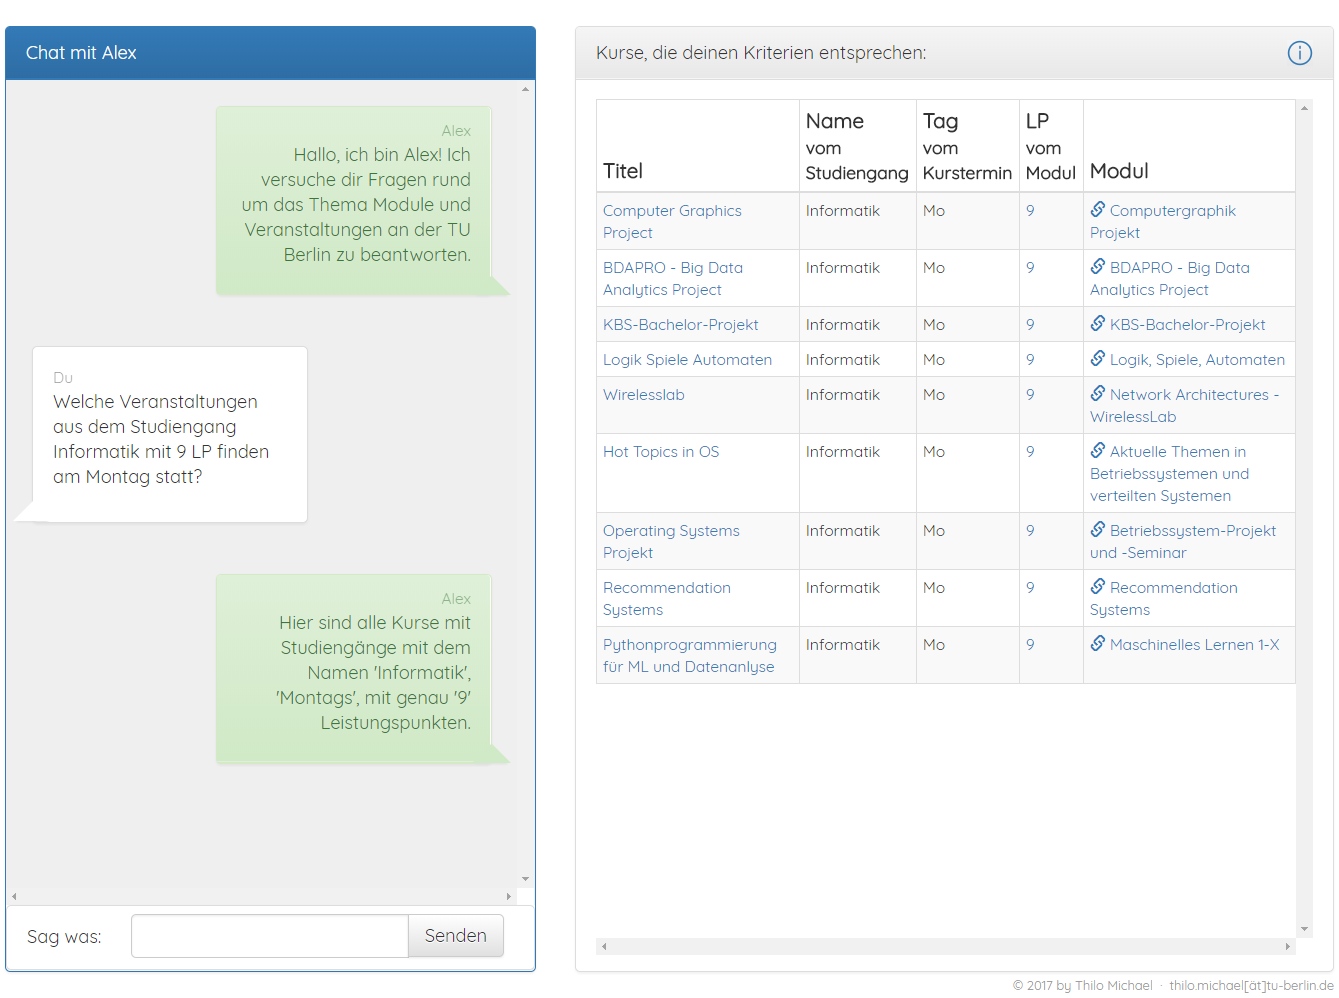
\includegraphics[width=\textwidth]{images/alex_screencapture}
	\vspace{.1em}
	\caption[User Interface of \Alex]{The user interface of \Alex. The left section contains the conversation with the agent and a user entry field. The right section shows the result of the generated database query in tabular form.\\In this example, the user asked for all courses of the subject \i{computer science} that provide 9 ECTS and are scheduled on a Monday. The agent answered accordingly and provided a list of 9 courses that fulfill the conditions.\\This image was captured on 21st April 2018.}
	\label{f.alex_ui}
\end{figure}

\Alex\ consists of several processing modules:

\begin{itemize}
	\item The \b{tagging module} uses a hidden Markov model to calculate the parts of speech for the user input, later described in Chapter \ref{c.alex.hmm}
	\item The \b{query generation module} composes actual SQL queries from the tagged output data by recognizing the requested model and the return type
	\item The \b{filter extraction module} refines the query generator and provides constraint handling for it
	\item The \b{response generation module} formulates answers for the user input using natural language by processing the generated query, the recognized model and the conversation state.
\end{itemize}

Moreover, \Alex\ provides a user interface, which utilizes web technologies and can be accessed via a web browser. Figure \ref{f.alex_ui} shows the user interface, in which the user asked a question and the agent returned the result in tabular form and answered accordingly.

The focus of this thesis lies on the tagging module. As outlined in Chapter \ref{c.introduction.scope}, the main objective is to replace the hidden Markov model by artificial neural networks. Both approaches with their historical context are introduced in the following.

\subsection{The Hidden Markov Model}\label{c.introduction.related.hmm}
The hidden Markov model (HMM) is a probabilistic finite state machine that solves general classification problems. It uses the observable output data of a system to derive hidden information from it. Among other applications, HMMs are used especially for speech recognition tasks.

The preliminary work for HMMs was done by R. L. Stratonovich. He first described conditional Markov processes in 1960 \cite{stratonovich1960}, which were used in the following years to describe simple Markov Models and later hidden Markov models (see Baum et. al. \cite{baum1966}\cite{baum1967}). The latter became a popular solution for automatic recognition of continuous speech \cite{baker1975} along with other applications, such as pattern recognition in general, the analysis of biological sequences (e.g. DNA) \cite{bishop1986} and part-of-speech tagging \cite{kupiec1992}.

\subsection{The Artificial Neural Network Model}\label{c.introduction.related.nn}
Artificial neural networks are networks that process information inspired by the biological nervous system. They consist of connected computational units, typically arranged in different layers. Such a unit (also called \i{artificial neuron}) can make calculations based on its inputs and pass the result to the neighboring units. These connections are weighted, so that the weight can be adjusted depending on the activity of the unit. Thus, a model based on the features of the input data can be created.

Following research by W. McCulloch, W. Pitts \cite{mcculloch1943} and D. Hebb \cite{shaw1986} on arithmetical learning methods, inspired by the connections of neurons in the 1940s, M. Minsky built the first neural network learning machine called SNARC (\i{Stochastic Neural Analog Reinforcement Computer)}\cite{crevier1993} in 1951.

In the late 1950s, F. Rosenblatt developed the \i{Mark I Perceptron} computer and published a theorem of convergence of the perceptron\cite{rosenblatt1958} in 1958. He coined the term \i{perceptron} for an algorithm that is able to learn the assignment of input data to different classes. The perceptron represents a simple artificial neural network initially containing one single neuron\footnote{Chapter \ref{c.postagging.fnn} and Chapter \ref{c.postagging.rnn} explain the architecture of different neural network structures in detail}. F. Rosenblatt stated that any function that is representable by the model can be learned with the proposed learning method. In 1960, B. Widrow presented the ADALINE\footnote{ADALINE is an acronym for Adaptive Linear Neuron} model of a neural network, for which input weights could already be adjusted by the learning algorithm \cite{widrow1960}.

A publication of M. Minsky and S. Papert \cite{minsky1969} from 1969 analyzed and exposed some significant limitations of the basic perceptron. They pointed out that it is impossible to learn functions without linear separability (e.g. the exclusive-or problem). Due to these limitations and the fact that the processing power of computers at the time was not sufficient for larger neural networks, research interest in artificial neural networks decreased in the following years.

In 1982, J. Hopfield presented a previously described neural network with feedback (known as \i{Hopfield network}), that was able to solve optimization problems like the \i{Traveling Salesman Problem}\footnote{The problem of the traveling salesman or round trip problem: The order of places to be visited once should be chosen in such a way that the distance covered is minimal, whereby the last place is the starting point again (round trip).}. Neural network approaches started to receive more attention again, also due to the first processors based on transistor technology (microprocessors) being introduced to the market in the early 1970s, replacing the previously used tube technology in the following years, which made computers smaller and cheaper and increased their processing capacity.

For the task of POS tagging, neural network models were now able to outperform HMM based taggers. H. Schmid created and trained a multilayer Feed-forward neural network in 1994 and was able to show that it performed better than an HMM tagger \cite{schmid1994} at that time. In 2000, Ma et. al. ran a series of comparative experiments that proved that results of a neural network tagger can be superior to those of statistical models like the HMM \cite{ma2000}.

\section{Structure of this Thesis}\label{c.introduction.structure}
This first chapter outlined the subject of natural language processing and part-of-speech tagging in general as an introduction.

The second chapter describes the structure and functionality of the already existing ACA, \Alex, with the main focus on its language model and tagging interface.

Chapter \ref{c.postagging} explains the implementation of a part-of-speech tagging system using two different neural network approaches.

The training of the language models including the retrieval of training data and tuning training parameters is described in Chapter \ref{c.training}.

Chapter \ref{c.evaluation} illustrates the evaluation of each language model with a generated test set and their comparisons.

In conclusion, Chapter \ref{c.conclusion} discusses and summarizes the evaluation results and presents an outlook on future work.

% ===================================================================================
\chapter{\Alex: Artificial Conversational Agent}\label{c.alex}
\i{Design and Implementation of an Advisory Artificial Conversational Agent} by T. Michael \cite{michael2016} provides a detailed and comprehensive description of \Alex\ as a compilation of different modules. This chapter focuses on components that are relevant for language processing and were therefore adapted during this thesis: The retrieval and processing of training data (Chapter \ref{c.alex.data}), the hidden Markov model tagger (Chapter \ref{c.alex.hmm}) and the tagging interface (Chapter \ref{c.alex.tagging}).

\section{System Overview}\label{c.alex.overview}
The modular structure of \Alex\ facilitates the separation of different functions and therefore simplifies the replaceability of certain functionalities. Besides a module crawler for current data retrieval of web content for the database and a front-end interface module, \Alex\ offers a tagging module. This module enables the training of a language model as well as the assignment of tags to words of a given input sentence.

Figure \ref{f.alex.components} shows the original architecture of \Alex. The following components are part of the tagging module and are adapted or replaced (emphasized with an orange border in Figure \ref{f.alex.components}) in this thesis:

\begin{itemize}
	\item The \b{HMM Training Data} is replaced by training data that was generated with improved training sentence templates (see Chapter \ref{c.training.data} for a comprehensive explanation)
	\item \b{Training Data Loading and Slot Filling} are used to generate the new training data
	\item The \b{HMM Tagger} is replaced by a neural network based tagger
	\item \b{Part of Speech Tagging} of input sentences is realized by the tagging function of the new tagger
\end{itemize}

\begin{figure}[H]
	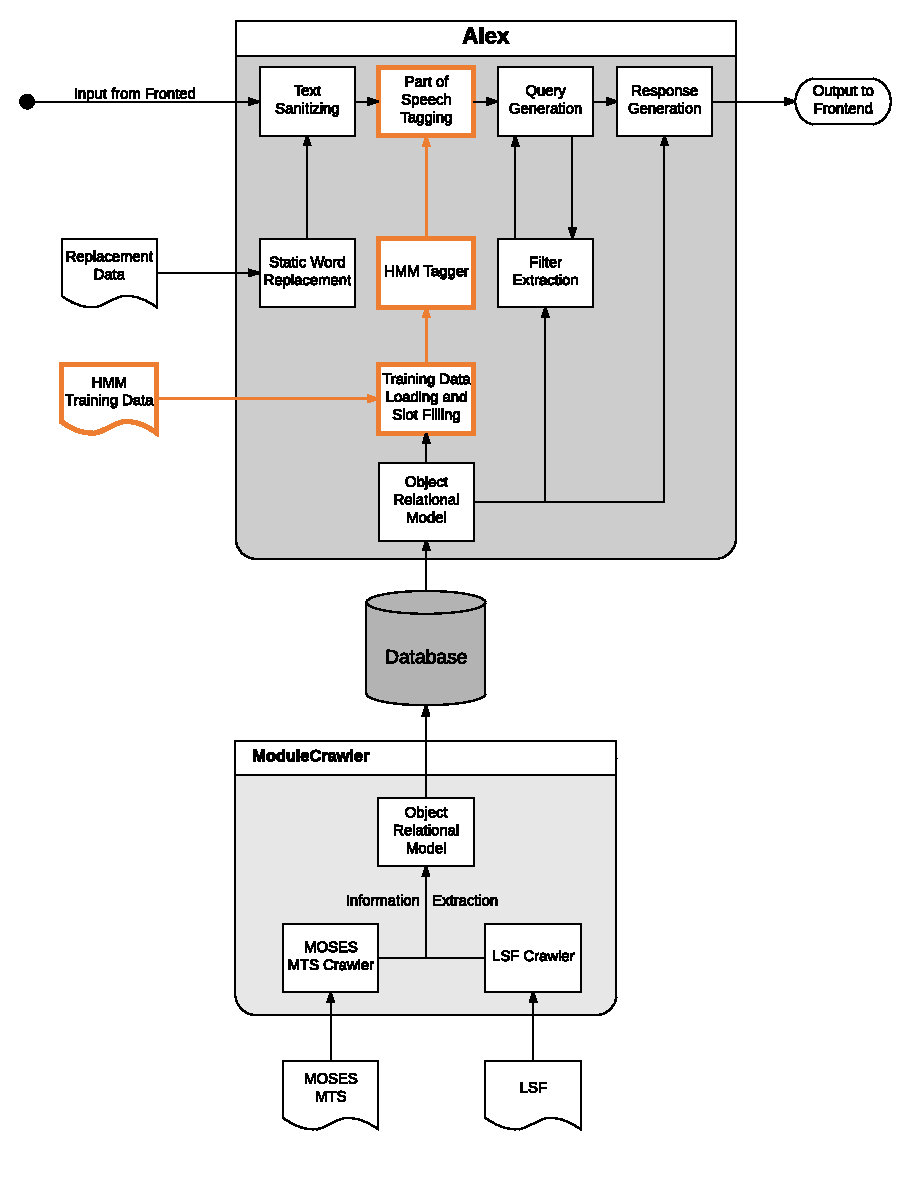
\includegraphics[width=\textwidth]{images/alex_components}
	\caption[Component Overview of \Alex]{Overview of all components of \Alex. The orange borders identify components that lie within the scope of this thesis and have been adapted or replaced. Original graphic by T. Michael \cite{michael2016}}
	\label{f.alex.components}
\end{figure}

\section{Training Data}\label{c.alex.data}
In order to teach \Alex\ to assign tags to words correctly, depending on their context, appropriate training data is required. The training data for \Alex\ proposed by T. Michael consists of \tt{556,111} tagged sentences generated with \tt{72} manually created sentence templates.

A sentence template is a sentence that provides the structure of a possible tagged training sentence with proper syntax for slot filling. It consists either of special placeholders for specific data from the database (e.g. module titles), inline choices (e.g. the same sentence with each day of the week) or a marker to simply duplicate the sentence. The different slot filling forms can be combined or used multiple times in one sentence\footnote{T. Michael describes the training data structure in detail in Chapter 3.4.2 of \i{Design and Implementation of an Advisory Artificial Conversational Agent} \cite{michael2016}.}.

For training the neural network models in this thesis, this slot filling mechanism is adopted and improved for the training with artificial neural networks (see Chapter \ref{c.training}).

\section{The Hidden Markov Model Tagger}\label{c.alex.hmm}
As described in Chapter \ref{c.introduction.related.hmm} \ of the introduction, the hidden Markov model (HMM) is a statistical tool that uses observable output data of a system to derive hidden information from it. Areas of application are image processing, gesture recognition and natural language processing tasks, such as speech recognition in general and part-of-speech tagging in particular.

In case of POS tagging, the observable states of the HMM represent the given sequence of words, whereas the hidden states represent the corresponding parts of speech. The HMM calculates the joint probability of the whole sequence of hidden states based on transmission and output probabilities. Subsequently, it finds the maximum probability of all possible state sequences and determines as a result, which parts of speech most likely correspond to the words of the input sequence.

Figure \ref{f.hmm_structure} illustrates an example of a state sequence with three hidden states (part of speech tags) and the observed word sequence in an HMM. The calculation of the joint probability $P$ of the word sequence in this case is shown in Equation \ref{e.hmm_joint_probability}, as the product of transmission and output probabilities.

\begin{equation}
    P = p_{start}\cdot p_{out,1}\cdot p_{trans,1}\cdot p_{out,2}\cdot p_{trans,2}\cdot p_{out,3} \label{e.hmm_joint_probability}
\end{equation}

\vspace{1em}
\begin{figure}[H]
	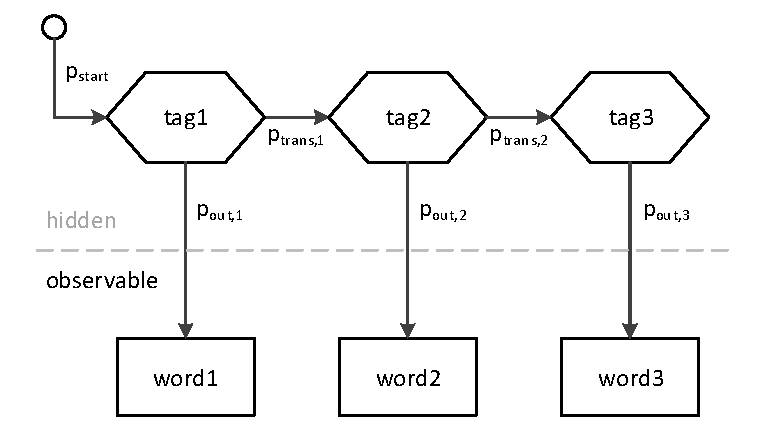
\includegraphics[width=\textwidth]{images/hmm_structure}
	\vspace{.8em}
	\caption[Structure of a Hidden Markov Model]{An example of a state sequence of three hidden states (tag1 -- tag3) and an observed sequence of three words (word1 -- word3) in a hidden Markov model. $p_{start}$ denotes the starting probability, $p_{trans}$ the transmission probabilities between hidden states and $p_{out}$ the output probabilities between a hidden state and an output.}
	\label{f.hmm_structure}
	\vspace{.8em}
\end{figure}

For the purpose of finding corresponding parts of speech to a given input sentence, an HMM is included in \Alex. According to T. Michael \cite{michael2016}, a tagging scheme was developed to extract exactly the information from user input that is needed to successfully create a database query and to return the information the user asked for. This tagging scheme was intentionally built to be domain independent, creating the opportunity to develop a version of \Alex\ for any topic based on an appropriate database and training data.

To maintain this universal applicability as well as the compatibility with other modules of \Alex, the neural network approaches presented in this thesis use the same tagging scheme \Alex\ already utilizes. For a better understanding of the evaluation results in Chapter \ref{c.evaluation}, Table \ref{t.tagging_scheme} gives an overview of the 6 different classes of tags that \Alex\ uses.

\begin{table}[H]
	\small\def\arraystretch{1.5}\begin{tabular}{ p{2mm} L{48mm} p{35mm} p{40mm} }
	\trule
	 & \textsc{Formats} & \textsc{Description} & \textsc{Example} \\
	\drule
	\tt{R} & \i{Return-tags}, describing data that is expected to be returned & \tt{R\_LIST} \newline \tt{R\_SINGLE} \newline \tt{R\_COUNT} & \i{"\b{Which} modules \dots"} \newline \i{"\b{Which} module \dots"} \newline \i{"\b{How many} modules \dots"} \\
	\mrule
	\tt{M} & \i{Model-tags}, describing the database model, e.g. \tt{M\_MTSModule} or \tt{M\_Course} & \tt{M\_[MODEL]} & \i{"Which \b{modules} \dots"} \newline \i{"Which \b{courses} \dots"} \\
	\mrule
	\tt{C} & \i{Constraint-tags}, filtering the result set, given a database model and corresponding field, e.g. \tt{C\_MTSModule:ects} & \tt{C\_[MODEL]:[FIELD]} & \i{"Modules with \b{6} ects \dots"} \\
	\mrule
	\tt{P} & \i{Property-tags}, indicating to include fields in the result set, e.g. \tt{P\_MTSModule:ects} & \tt{P\_[MODEL]:[FIELD]} & \i{"Modules with 6 \b{ects} \dots"} \\
	\mrule
	\tt{Q} & \i{Comparison-tags}, describing an equal, greater than or less than constraint & \tt{Q\_EQ} \newline \tt{Q\_LT} \newline \tt{Q\_GT} &  \i{"\dots\ with \b{exactly} 6 ects \dots"} \newline \i{"\dots\ \b{less than} 6 ects \dots"} \newline \i{"\dots\ \b{more than} 6 ects \dots"} \\
	\mrule
	\tt{X} & \i{Extra-tags}, describing words that are not relevant for the database query\tablefootnote{This can refer to words with no specific meaning (tagged with \tt{X}), words that have no meaning for the database query but for the system itself (e.g. the tag \tt{X\_HELP} for the word \i{"help"}) or words that lead to a particular constraint (such as the tag \tt{X\_Person:fullname} for the word \i{"Professor"}, leading to a name).} & \tt{X} \newline \tt{X\_[WORD]} \newline \tt{X\_[MODEL]:[FIELD]} & \i{"\b{and}"}, \i{"\b{of}"}, \i{"\b{is}"} \newline \i{"I need \b{help}"} \newline \i{"\b{Professor} John Doe"} \\
	\brule
	\end{tabular}
	\caption[Tagging Scheme Overview]{Overview of the tagging scheme used in \Alex, consisting of 6 different classes of tags with a total of 12 different formats. The examples contain \b{emphasized} words that belong to the corresponding tag formats. T. Michael \cite{michael2016} provides a detailed explanation of the tagging classes and its formats.}
	\label{t.tagging_scheme}
	\vspace{1ex}
\end{table}

\section{Tagging Interface}\label{c.alex.tagging}
As described in the previous chapter, the implementation of the tagging module of \Alex\ utilizes a hidden Markov model for part-of-speech tagging. \Alex\ uses an already existing implementation of the HMM Tagger from the Natural Language Toolkit (NLTK)\footnote{The Natural Language Toolkit is a collection of \i{Python} programming libraries for natural language processing, see \link{http://nltk.org}}, called \tt{HiddenMarkovModelTagger}.

To replace the existing tagger, a new tagger has to provide a class with two methods: \tt{train} and \tt{tag}. These methods are used to create the language model and apply it to unknown data.

The \tt{train} method creates a new instance of the tagger class, trains this class with the given training data and returns it. The training data itself must be a list of sentences, where a sentence is a list of tuples, containing each word of this sentence and its corresponding tag. The following exemplifies the structure of the training input data containing two sentences, where each word is tagged with \i{TAG}:

\lstinputlisting[language=JSON, label={l.trainingdata}]{listings/method-train.example}

The \tt{tag} method attaches a tag to each word of an input sentence, according to the previously trained language model. The input has to be an unknown sentence formatted as a simple list of words:

\lstinputlisting[language=JSON]{listings/method-tag-input.example}

The output is a corresponding list of tuples containing a word and its assigned tag:

\lstinputlisting[language=JSON]{listings/method-tag-output.example}


% ===================================================================================
\chapter{Part-of-Speech Tagging with Neural Networks}\label{c.postagging}
A part-of-speech tagger is a system which automatically assigns the part of speech to words using contextual information. Potential applications for part-of-speech taggers exist in many areas of computational linguistics including speech recognition, speech synthesis, machine translation or information retrieval in general.

Chapter \ref{c.introduction.related.nn} introduced neural networks as a possible approach for POS tagging. The current chapter presents two different neural network architectures and their implementation that is later used to train and evaluate language models with the objective of comparing their POS tagging accuracy with the accuracy of the HMM tagger that \Alex\ uses.

In general, a neural network represents a mathematical function, which is able to assign specific output data to corresponding input data. This assignment is learned by processing input data whose output is known. Thus, it belongs to the category of supervised learning\footnote{\i{Supervised Learning} describes the process of gaining knowledge with the help of labeled data. Depending on the capability of the supervised learning algorithm to generalize from the given data, this knowledge can then be applied to unknown data.}.

The network itself emerges from the interconnection of nodes (the artificial neurons), that are usually arranged in different layers. Each node represents a non-linear\footnote{The non-linearity is important because linear functions cannot describe some mutual exclusive feature combinations.} activation function that calculates an output, depending on the sum of its inputs. Possible activation functions are the sigmoid function, the hyperbolic tangent or the maximum function.

The training effect is achieved by weighting the connections of the nodes and adjust these weights during training. The weights of neural networks are typically represented by real numbers. The adjustments are defined by a learning algorithm that utilizes a particular learning method. Using the initial or current weights of the network, an error (also called \i{loss}) between the prediction and the given label can be computed on the last layer (the output layer) with the help of a corresponding loss function. The training objective is to minimize the loss function of the current state of the network and adjust the weights accordingly. This can be achieved by using \i{backpropagation} with \i{stochastic gradient descent} (SGD).

The POS tagging task requires the processing of words which are represented as character strings. For computational processing, each word is mapped to an integer value (the word id).

\section{Feed-forward Neural Network Model}\label{c.postagging.fnn}
Feed-forward neural networks are a common type of ANNs, that consist of an input and an output layer with one or more hidden layers in between. An FNN propagates information through the network only in the forward direction, from the input to the output layer.

\subsection{Architecture}\label{c.postagging.fnn.architecture}
The FNN architecture that is used in this thesis is shown in Figure \ref{f.fnn.structure}. The current word and the configured number of preceding words are each converted into word embeddings\footnote{Word embeddings are mathematical representations of words, usually presented as a vector of real numbers. While one-hot encoded word vectors have the size of the vocabulary, word embeddings maintain a dimensionality reduction to improve performance while maintaining feature information.}. These embeddings are reshaped to one vector, called the feature vector, which serves as the input layer for the neural network. The FNN contains one hidden layer, which is connected to the input layer with weight matrix $V$. The output layer represents the set of existing POS tags and is connected to the hidden layer with weight matrix $W$.

For each word of every sentence of the training corpus, a feature vector is built and the data is sequentially propagated to both the hidden and the output layer, predicting a POS tag for the current word and calculating the current loss and accuracy. After propagating the error back to adjust the weights and reduce the loss, the next training step is executed.

The outputs of the hidden layer are typically computed with the rectified linear activation function (the \i{rectifier}). These nodes are therefore also called \i{rectified linear units} (RELUs). However, the effect of 8 different activation functions is examined in this thesis too. Figure \ref{f.postagging.activation} illustrates the qualitative plot of each function. The presented activation functions can be separated into two different types of nonlinearities: \tt{RELU}\footnote{\i{Rectified Linear Unit}, Nair et. al. \cite{nair2010}}, \tt{RELU6} and \tt{SELU}\footnote{\i{Scaled Exponential Linear Units}, Klambauer et. al. \cite{klambauer2017}} are continuous functions but not everywhere differentiable, the other functions (\tt{ELU}\footnote{\i{Exponential Linear Units}, Clevert et. al. \cite{clevert2015}}, \tt{SIGMOID}\footnote{Also known as Logistic function or SoftStep}, \tt{TANH}, \tt{SOFTPLUS}\footnote{Glorot et. al. \cite{glorot2011}} and \tt{SOFTSIGN}\footnote{Bergstra et. al. \cite{bergstra2009}}) are continuously differentiable.

\begin{figure}[H]
\centering
\subcaptionbox{\tt{RELU}\label{f.postagging.activation.relu}}
{\includegraphics[width=0.325\textwidth]{images/activation_relu}}
\subcaptionbox{\tt{RELU6}\label{f.postagging.activation.relu6}}
{\includegraphics[width=0.325\textwidth]{images/activation_relu6}}
\subcaptionbox{\tt{ELU}\label{f.postagging.activation.elu}}
{\includegraphics[width=0.325\textwidth]{images/activation_elu}}
\subcaptionbox{\tt{SIGMOID}\label{f.postagging.activation.sigmoid}}
{\includegraphics[width=0.325\textwidth]{images/activation_sigmoid}}
\subcaptionbox{\tt{TANH}\label{f.postagging.activation.tanh}}
{\includegraphics[width=0.325\textwidth]{images/activation_tanh}}
\subcaptionbox{\tt{SELU}\label{f.postagging.activation.selu}}
{\includegraphics[width=0.325\textwidth]{images/activation_selu}}
\subcaptionbox{\tt{SOFTPLUS}\label{f.postagging.activation.softplus}}
{\includegraphics[width=0.325\textwidth]{images/activation_softplus}}
\subcaptionbox{\tt{SOFTSIGN}\label{f.postagging.activation.softsign}}
{\includegraphics[width=0.325\textwidth]{images/activation_softsign}}
\vspace{1em}
\caption[Activation Functions]{Qualitative illustration of 8 different activation functions that provide different types of nonlinearities. \tt{RELU}, \tt{RELU6} and \tt{SELU} are continuous but not everywhere differentiable functions, the other functions are continuously differentiable.}
\label{f.postagging.activation}
\end{figure}

\begin{figure}[ht]
	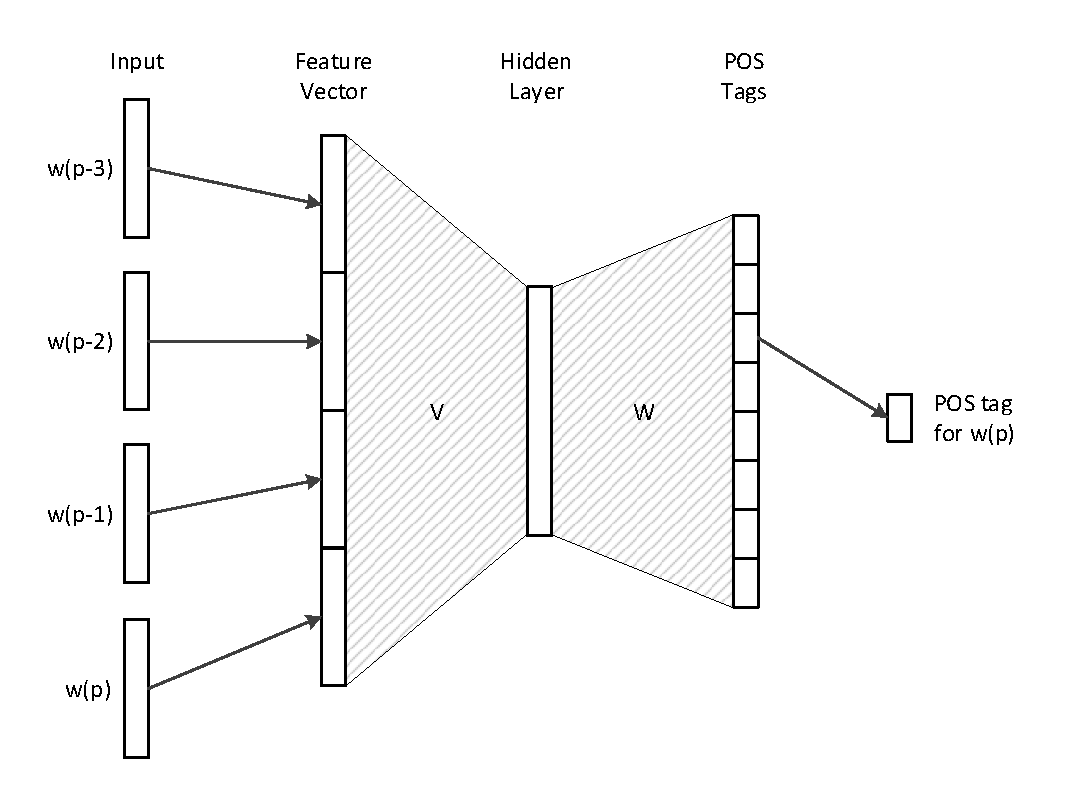
\includegraphics[width=\textwidth]{images/fnn_structure}
	\caption[Structure of a Feed-forward Neural Network]{The structure of a feed-forward neural network. The feature vector is built by the embeddings of the corresponding input word at position $p$ and by its 3 preceding words (the number of predecessors may vary, of course). $V$ and $W$ are weight matrices with respective matrix dimensions of $\textsf{feature vector size} \times \textsf{hidden layer size}$ for $V$ and $\textsf{hidden layer size} \times \textsf{number of POS tags}$ for $W$.}
	\label{f.fnn.structure}
\end{figure}

\subsection{Implementation}\label{c.postagging.fnn.implementation}
To implement the presented FNN architecture, the open source machine learning framework \i{TensorFlow}\footnote{TensorFlow is a library written in Python, that is utilized for high performance numerical computations especially for the area of machine learning. In this thesis, TensorFlow version 1.8 is used.\\See the official TensorFlow website: \link{https://www.tensorflow.org}} is used. In the following descriptions, all functions starting with \tt{tf} are functions from the TensorFlow library.

The nodes of the input layer are populated by the feature vector. To create the feature vector, an embedding matrix with the dimensions of $\textsf{vocabulary size} \times \textsf{embedding size}$ is created and initially filled with random normal distributed values\footnote{The generated values follow a normal distribution with mean of 0 and standard deviation of 0.1, except that values whose magnitude is more than two standard deviations from the mean are dropped (truncated) and re-picked. See the TensorFlow documentation.}, using the \tt{tf.truncated\_normal()} function. This matrix is used to retrieve the vectors for the current word and its predecessors via \tt{tf.nn.embedding\_lookup} and reshape them to one single vector, the feature vector. Figure \ref{f.fnn.feature} illustrates the creation of the feature vector.

\begin{figure}[ht]
	\vspace{1.5em}
	\hspace{-1.5em}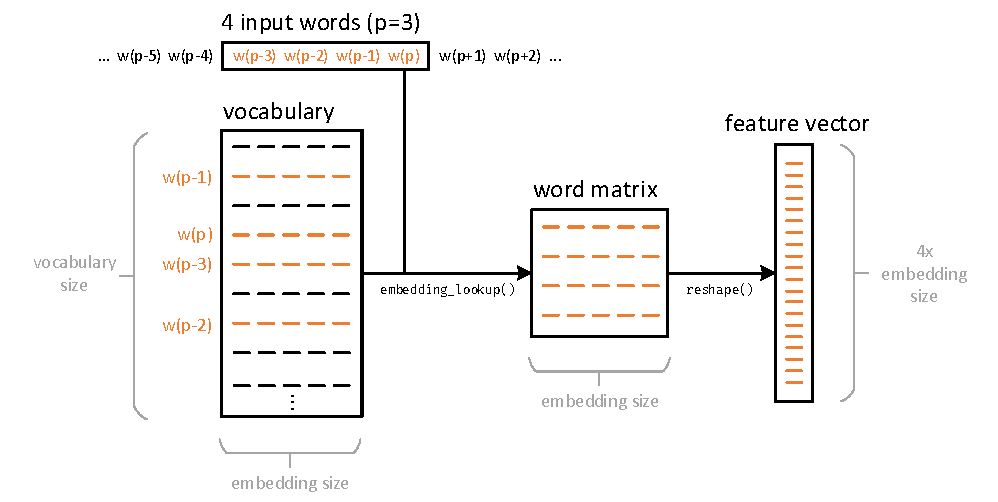
\includegraphics[width=1.1\textwidth]{images/feature_vector}
	\caption[Creation of the feature vector]{An example of the creation of a feature vector for the FNN using \tt{3} preceding words and the current word.}
	\label{f.fnn.feature}
	\vspace{.5em}
\end{figure}

The hidden layer nodes are also initialized with random normal distributed values. Their outputs are computed with one of the activation functions presented in Figure \ref{f.postagging.activation}. Table \ref{t.postagging.activation} lists the activation functions with their respective computation formula and the corresponding TensorFlow function.

\begin{table}[!ht]
	\centering\small\def\arraystretch{1.5}\begin{tabular}{ p{23mm} p{62mm} l }
	\trule
	\textsc{Name} & \textsc{Definition} & \textsc{TensorFlow} \\
	\srule
	\tt{RELU} & $a(x)=\max(x,0)$ & \tt{tf.nn.relu()} \\
	\midrule
	\tt{RELU6} & $a(x)=\min(\max(x,0),6)$ & \tt{tf.nn.relu6()} \\
	\midrule
	\tt{ELU} & $f(x)=\begin{cases}e^x-1,& \text{if } x<0\\x, & \text{otherwise}\end{cases}$ & \tt{tf.nn.elu()} \\
	\midrule
	\tt{SIGMOID} & $f(x)=\frac{1}{1+e^{-x}} $ & \tt{tf.nn.sigmoid()} \\
	\midrule
	\tt{TANH} & $f(x)=\tanh{x} $ & \tt{tf.nn.tanh()} \\
	\midrule
	\tt{SELU} & $f(x)=\lambda\begin{cases}\alpha (e^x-1),& \text{if } x<0\\x, & \text{otherwise}\end{cases} $ & \tt{tf.nn.selu()} \\
	\midrule
	\tt{SOFTPLUS} & $f(x)=\ln{(e^x+1)} $ & \tt{tf.nn.softplus()} \\
	\midrule
	\tt{SOFTSIGN} & $f(x)=\frac{x}{|x+1|} $ & \tt{tf.nn.softsign()} \\
	\bottomrule
	\end{tabular}
	\vspace{1em}
	\caption[Activation Functions]{Definitions and TensorFlow Implementations of 8 different activation functions.}
	\label{t.postagging.activation}
\end{table}

Finally, the values for the output layer (the logits) are computed using a matrix multiplication of the outputs of the RELUs and the weight matrix \tt{W} using the \tt{tf.matmul()} function. Subsequently, the loss can be calculated by computing the sparse softmax cross entropy between input labels and logits, using the \tt{tf.nn.sparse\_softmax\_cross\_entropy\_with\_logits()} function.

The predictions are calculated with the \tt{tf.argmax()} function, that reduces the logits to the largest value, which represents the predicted POS tag. The function \tt{tf.train.AdamOptimizer()}\footnote{The Adam algorithm is an optimizer that was proposed by D. Kingma et. al. in 2014 \cite{kingma2014}. It provides a computationally efficient gradient-based optimization of stochastic objective functions.} enables backpropagation with stochastic gradient descent to optimize the computations and results during training.

The implementation of the FNN POS tagger that was developed for this thesis is based on an existing TensorFlow POS tagger implementation by M. Rahtz\footnote{The POS tagger is licensed under GNU GPL v3.0 and was retrieved on 15th January 2018.\\\link{https://github.com/mrahtz/tensorflow-pos-tagger}}.

\section{Recurrent Neural Network Model}\label{c.postagging.rnn}
Similar to FNNs, recurrent neural networks (RNNs) also consist of an input, a hidden and an output layer. The main difference is that information is not only propagated forward linearly, but that information from previous training steps are also taken into account in RNNs.

\subsection{Architecture}\label{c.postagging.rnn.architecture}
Figure \ref{f.rnn.structure} illustrates the architecture of an RNN, which was implemented for this thesis. Unlike the FNN, the RNN only uses word ids as input features and does not utilize word embeddings. It contains one hidden layer, which is populated with the current input word on the one hand and by the output of the hidden layer of a previous training step on the other hand. This makes the RNN capable of memorizing information from the past. This capability can also be described as a long short-term memory (\i{LSTM}), emphasized in orange in Figure \ref{f.rnn.structure}. The output layer represents the set of existing POS tags and is connected to the hidden layer with weight matrix
$W$.

Each word of every sentence of the training corpus represents an input feature, which is propagated to the hidden and the output layer together with information from previous training steps. Similar to the processing of FNNs, the POS tag is predicted for the current word and the current loss and accuracy are calculated. After propagating the error back to adjust the weights and reduce the loss, the next training step is executed, taking the current training step into account.

The outputs of the hidden layer are calculated utilizing the same activation functions that were used for the FNN (see Figure \ref{t.postagging.activation}).

\begin{figure}[ht]
	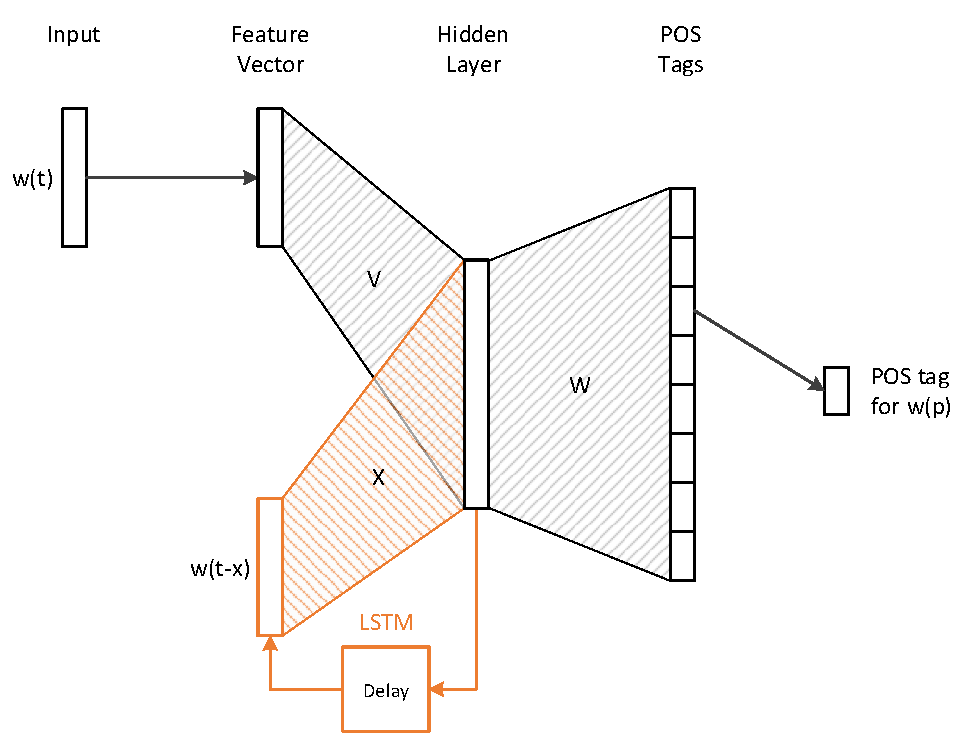
\includegraphics[width=\textwidth]{images/rnn_structure}
	\caption[Structure of a Recurrent Neural Network]{The structure of a recurrent neural network. The feature vector is the initial vector of the corresponding input word at time $t$. The output of the hidden layer from previously trained words (here at time $t-x$) is populated back into the same hidden layer for the current word. $V$, $X$ and $W$ are weight matrices with respective matrix dimensions of $\textsf{feature vector size} \times \textsf{hidden layer size}$ for $V$, $\textsf{hidden layer size} \times \textsf{hidden layer size}$ for $X$ and $\textsf{hidden layer size} \times \textsf{number of POS tags}$ for $W$.}
	\label{f.rnn.structure}
\end{figure}

\subsection{Implementation}\label{c.postagging.rnn.implementation}
The implementation of the proposed RNN architecture utilizes the TensorFlow library as well. Besides the word id of the current word, the input layer has an additional dimension describing the number of past training steps that are considered for the current training step.

The hidden layer is built using \tt{tf.nn.rnn\_cell.LSTMCell()}\footnote{This function uses an implementation proposed by S. Hochreiter et. al. in 1997 \cite{hochreiter1997}.}, a function that creates a long short-term memory (LSTM) cell for recurrent networks which is then used in \tt{tf.nn.dynamic\_rnn()} to compute the logits for the output layer.

Loss, predictions and accuracy are implemented in the same way as in the FNN. In addition, the same optimizer (\tt{tf.train.AdamOptimizer()}) is used.

% ===================================================================================
\chapter{Training of Language Models}\label{c.training}
An optimal language model using the neural network approach proposed in this thesis, requires as much annotated training data as possible. The following sections describe the generation of tagged training data and the training of different language models, due to parameter variation, based on this generated training corpus.

\section{Training Data Corpus}\label{c.training.data}
To create a training corpus with tagged sentences, the already existing sentence template set of \Alex\ is used as the basis for an improved and extended template set. In addition, a log of user input data\footnote{The log data that was available for this thesis started on 30th of August, 2017 until 27th of April, 2018 and contained 1293 entries of user input.} provides useful information on possible input sentences, that are not yet considered in the template set.

As described in Chapter \ref{c.alex.data}, the HMM tagger of \Alex\ uses 72 sentence templates to generate annotated training data. However, the distribution of the generated sentences is highly unbalanced. Due to the combination of placeholders for different database fields and models, which are semantically meaningless, a huge number of training sentences exist that are only partially suitable for training.

An analysis of the generated training corpus that was used to train the HMM tagger showed that one single template of the 72 sentence templates created more than 84\% of the whole training corpus. This sentence template is the following\footnote{The corresponding English translation of this sentence template is: \i{Which modules are held by Professor <firstname> <lastname>}}:

\vbox{\begin{Verbatim}[fontsize=\scriptsize]
Welche   Module  werden von   Prof   {Person:firstname} {Person:lastname} angeboten
\end{Verbatim}
\vspace{-6mm}
{\color{gray}\begin{Verbatim}[fontsize=\scriptsize]
R_LIST M_MTSModule  X    X  X_Person C_Person:fullname  C_Person:fullname     X
\end{Verbatim}
}}

It combines all first names and all last names of each existing person in the database, leading to a huge number of name combinations that do not exist.

Another example is the combination of study program degrees and program names. This combination exists in 5 of the 72 sentence templates, i.e. all degrees are assigned to all study programs 5 times, although not every combination exists in reality. The following is an example of one of these sentence templates\footnote{The corresponding English translation of this sentence template is: \i{Which modules can I attend to in <program-degree> <program-name>}}:

\vbox{\begin{Verbatim}[fontsize=\scriptsize]
Welche   Module    kann ich  im  {Program:degree}  {Program:name} belegen
\end{Verbatim}
\vspace{-6mm}
{\color{gray}\begin{Verbatim}[fontsize=\scriptsize]
R_LIST M_MTSModule  X    X   X   C_Program:degree  C_Program:name    X
\end{Verbatim}
}}

To address this issue, the following adjustments were made for the new template set were made:

\begin{itemize}
	\item Because the number of occurrences is very low in the log database, the slot \tt{\{Person:firstname\}} was removed completely from the sentence template, which limits the user input to last names only\footnote{This might seem like a degradation but is justified by the fact, that only 3 of 1293 log entries (0.2\%) even contained a first name, always followed by the last name. In this specific use case, where all persons are professors and lecturers, using the last name only is a reasonable approach.}.
	\item The slot \tt{\{Program:degree\}} was partly replaced by the inline choice \tt{(bachelor|master|diplom)}, which included the main terms requested in the logs.
\end{itemize}

Furthermore, wording referring to linking words and actions, which occurs in the logs, was improved with the help of inline choices. Table \ref{t.improved_sentence_templates} shows an excerpt of those improvements, comparing the previous and the new sentence template:

\begin{table}[H]
	\small\def\arraystretch{1.5}\begin{tabular}{ L{43mm} L{43mm} p{43mm} }
	\trule
	\textsc{Previous Template} & \textsc{New Template} & \multicolumn{1}{L{43mm}}{\textsc{English Equivalent}} \\
	\drule
	Alle Module \b{vom} \{Program:degree\} \{Program:name\} & Alle Module \b{(vom|von|in|im)} \{Program:degree\} \{Program:name\} & \multicolumn{1}{L{43mm}}{\i{All modules \b{(of|in)} \{Program:degree\} \{Program:name\} }} \\
	\mrule
	Welche Module werden von Prof \{Person:firstname\} \{Person:lastname\} \b{angeboten} & Welche Module werden von Professor \{Person:lastname\} \b{(unterrichtet| angeboten|gehalten)} & \multicolumn{1}{L{43mm}}{\i{Which modules are \b{(taught|offered|held)} by Professor \{Person:lastname\} }} \\
	\mrule
	\b{Wieviele} LP \b{hat} das Modul \{MTSModule:title\} & \b{(Wieviele|Wieviel)} LP \b{(hat|bringt)} das Modul \{MTSModule:title\} & \multicolumn{1}{L{43mm}}{\i{\b{How many} ects does the module \{MTSModule:title\} \b{(have|yield)} }} \\
	\mrule
	\b{Informationen} \b{zu} Modul {MTSModule:title} & \b{(Informationen|Details| Mehr)} \b{(zu|zum)} Modul \{MTSModule:title\} & \multicolumn{1}{L{43mm}}{\i{\b{(Information|details| more)} \b{of} the module \{MTSModule:title\} }} \\
	\brule
	\end{tabular}
	\caption[Sentence Template Improvements]{An excerpt of the extension and improvement of the sentence templates by using inline choices. The last column provides the corresponding English translation for the new sentence template.}
	\label{t.improved_sentence_templates}
	\vspace{1em}
\end{table}

All in all, the new set of sentence templates contains 36 templates, which are exactly the same as in the old set, 29 templates that were slightly modified or extended while maintaining the same tag sequence and 35 new sentence templates. The latter were created according to a sentence structure that was found in the logs but not in the previous template set. Therefore, the new set contains a total of 100 sentence templates (including single word templates) and can be found in Appendix \ref{c.appendix.sentencetemplates}.

The resulting training data corpus used in this thesis contains 218.700 tagged sentences consisting of 2.038.490 words, with a vocabulary of 9141 words.

\section{Parameter Tuning}\label{c.training.tuning}
In order to achieve better evaluation results and therefore more words that are tagged correctly, several training parameters are changed. To see the effect of the training parameters on the accuracy of the resulting language model, one parameter was altered while keeping all other parameters constant. The gained knowledge from the evaluation of these models was subsequently used to train further models with tuned parameters.

For the training of the FNN models, the following 5 parameters were considered:

\begin{itemize}
	\item \b{Number of past words} (\i{\b{p}}) specifies how many preceding words should be considered for the training of the current word
	\item \b{Embedding size} (\i{\b{e}}) describes the dimension of the word embeddings that were created for each word of the vocabulary during training
	\item \b{Hidden layer size} (\i{\b{s}}) characterizes the dimension of the hidden layer, i.e. the number of neurons that constitute the hidden layer
	\item \b{Number of training epochs} (\i{\b{n}}) indicates how often the whole training corpus is processed during training
	\item \b{Activation function} (\i{\b{a}}) constitutes a mathematical function that processes input information on each artificial neuron of the network to calculate a corresponding output
\end{itemize}

Based on these 5 parameters, Table \ref{t.training.tuning.fnn} shows different parameter combinations. The emphasized cells show the respective parameter that is variable. The first 4 training groups represent the basic training process to demonstrate the effect of each parameter in general. The subsequent training groups included additional parameter combinations, taking into account the evaluation results of the first training groups.

The resulting number of models is 99; however, due to an overlap in configurations of the training groups, the total number of distinct models to be trained with the FNN is 93.

\begin{table}[H]
	\centering\small\def\arraystretch{1.5}\begin{tabular}{ c c >{\centering}p{20mm} >{\centering}p{18mm} >{\centering}p{18mm} c c }
	\trule
	\textsc{Group} & $p$ & $e$ & $s$ & $n$ & $a$ & \textsc{Models} \\
	\drule
	\i{1} & \b{0--12} & 50 & 100 & 1 & relu & \i{13} \\
	\mrule
	\i{2} & 1 & \b{1, 5, 10, 25, 50--700}\tablefootnote{With a step size of 50\label{fifty}} & 100 & 1 & relu & \i{18} \\
	\mrule
	\i{3} & 1 & 50 & \b{10, 25, 50--1000}\footref{fifty} & 1 & relu & \i{22} \\
	\mrule
	\i{4} & 1 & 50 & 100 & \b{1, 5, 10, 20--140}\tablefootnote{With a step size of 20} & relu & \i{10} \\
	\srule
	\i{5} & 1 & \b{200--600}\footref{fifty} & 350 & 1 & relu & \i{9} \\
	\mrule
	\i{6} & 1 & 250 & \b{200--600}\footref{fifty} & 1 & relu & \i{9} \\
	\mrule
	\i{7} & 1 & \b{50--500}\footref{fifty} & \b{50--500}\footref{fifty} & 5 & relu & \i{10} \\
	\mrule
	\i{8} & 1 & 250 & 350 & 5 & \b{relu, ...}\tablefootnote{The following 8 activation functions were considered: \ftt{RELU}, \ftt{RELU6}, \ftt{ELU}, \ftt{SIGMOID}, \ftt{TANH}, \ftt{SELU}, \ftt{SOFTPLUS} and \ftt{SOFTSIGN}. See Chapter \ref{c.postagging.fnn.architecture}} & \i{8} \\
	\brule
	\end{tabular}
	\vspace{.5em}
	\caption[Parameter combinations of FNN Models]{The parameter configuration for training the FNN models. The rows represent the training groups with the corresponding variable parameter (in bold), while the columns represent the single training parameters (\i{\b{p}} - number of past words, \i{\b{e}} - embedding size, \i{\b{s}} - hidden layer size, \i{\b{n}} - number of training epochs, \i{\b{a}} - activation function). The first column denotes the group number (for referencing training groups) whereas the last column shows the resulting number of models for each training group.}
	\label{t.training.tuning.fnn}
	\vspace{1em}
\end{table}

For the training of the RNN models, the following 4 parameters were considered:

\begin{itemize}
	\item \b{Number of time steps} (\i{\b{t}}) specifies how many past training steps should be considered for the training of the current word
	\item \b{Hidden layer size} (\i{\b{s}}) characterizes the dimension of the hidden layer (as in the FNN)
	\item \b{Number of training epochs} (\i{\b{n}}) indicates how often the whole training corpus is processed (as in the FNN)
	\item \b{Activation function} (\i{\b{a}}) constitutes a mathematical function (as in the FNN)
\end{itemize}

Based on these 4 parameters, Table \ref{t.training.tuning.rnn} shows different parameter combinations. The emphasized cells show the respective parameter that is variable. The resulting number of models is 40; however, due to an overlap in configurations of the training groups, the total number of models to be trained with the RNN is 38.

\begin{table}[ht]
	\vspace{2em}
	\centering\small\def\arraystretch{1.5}\begin{tabular}{ c c c c c c }
	\trule
	\textsc{Group} & $t$ & $s$ & $n$ & $a$ & \textsc{Models} \\
	\drule
	\i{9} & \b{0--12} & 50 & 1 & relu & \i{12} \\
	\mrule
	\i{10} & 1 & \b{10, 25, 50--500}\tablefootnote{With a step size of 50\label{fiftyrnn}} & 1 & relu & \i{12} \\
	\mrule
	\i{11} & 1 & 50 & \b{1, 5, 10, 20--100}\tablefootnote{With a step size of 20\label{twentyrnn}} & relu & \i{8} \\
	\srule
	\i{12} & 8 & 50 & 5 & \b{relu, ...}\tablefootnote{For the RNN the same 8 activation functions as for the FNN are used: \ftt{RELU}, \ftt{RELU6}, \ftt{ELU}, \ftt{SIGMOID}, \ftt{TANH}, \ftt{SELU}, \ftt{SOFTPLUS} and \ftt{SOFTSIGN}. See Chapter \ref{c.postagging.fnn.architecture}} & \i{8} \\
	\brule
	\end{tabular}
	\vspace{3mm}
	\caption[Parameter combinations of RNN Models]{The parameter configuration for the training of RNN models. The rows represent the training groups with the corresponding variable parameter (in bold), while the columns represent the single training parameters (\i{\b{t}} (number of time steps), \i{\b{s}} (hidden layer size), \i{\b{n}} (number of training epochs), \i{\b{a}} - activation function). The first column denotes the group number (for referencing training groups) whereas the last column shows the resulting number of models for each training group.}
	\label{t.training.tuning.rnn}
\end{table}

% ===================================================================================
\chapter{Evaluation and Comparison}\label{c.evaluation}
After giving a short description of how the evaluation tests were created, this chapter provides the evaluation results of all models of the 12 training groups that were trained using the variation of training parameters previously described. In addition to the results of each training group, the three different architectures (FNN, RNN and HMM) are compared.

\section{Test Design}\label{c.evaluation.test}
To evaluate the trained language models, two test sets were designed: a test set containing a selection of tagged sentences that actually exist in the training corpus (here called the \i{known test}) and a test set, for which the structure of the sentences in the known test was modified in a way that it remains semantically meaningful but does not occur in the training corpus (called the \i{unknown test}). The unknown test deliberately contains words, which do not exist in the vocabulary of the training corpus in order to assess how the model handles completely unknown data.

The sentences are divided into different topics to cover a wide range of possible input data. A reasonably balanced number of sentences was included in the different areas to ensure that the evaluation result does not depend on only one or two topics.

Table \ref{t.evaluation_topics_known} and Table \ref{t.evaluation_topics_unknown} show the different topics represented in the known and the unknown test set, the respective number of evaluation sentences and an example sentence to illustrate each topic. Both test sets combined include a total number of 1094 tagged test sentences, consisting of 7986 word-tag tuples.

\begin{table}[!ht]
	\centering\small\def\arraystretch{1.5}\begin{tabular}{ p{18mm} c L{95mm} }
	\trule
	\textsc{Topic} & \textsc{Sentences} & \multicolumn{1}{L{95mm}}{\textsc{Example}} \\
	\drule
	ECTS & \tt{44} & \multicolumn{1}{L{95mm}}{\i{Which modules have 6 ECTS}} \\
	\mrule
	Time & \tt{72} & \multicolumn{1}{L{95mm}}{\i{Which courses are on Tuesday}} \\
	\mrule
	Faculty & \tt{56} & \multicolumn{1}{L{95mm}}{\i{All modules of faculty 4}} \\
	\mrule
	Participants & \tt{54} & \multicolumn{1}{L{95mm}}{\i{Which courses are limited to 30 participants}} \\
	\mrule
	Persons & \tt{85} & \multicolumn{1}{L{95mm}}{\i{Which courses are taught by Professor Martinelli}} \\
	\mrule
	Program & \tt{60} & \multicolumn{1}{L{95mm}}{\i{I'm searching for all modules of the computer science program }} \\
	\mrule
	Modules & \tt{80} & \multicolumn{1}{L{95mm}}{\i{Modules with the title Cognitive Algorithms}} \\
	\mrule
	Chair & \tt{50} & \multicolumn{1}{L{95mm}}{\i{All modules of institute Media Science}} \\
	\mrule
	Exam & \tt{32} & \multicolumn{1}{L{95mm}}{\i{Courses with Group Lecture as examination}} \\
	\mrule
	Courses & \tt{45} & \multicolumn{1}{L{95mm}}{\i{When does Internet Security take place}} \\
	\mrule
	Locations & \tt{42} & \multicolumn{1}{L{95mm}}{\i{All courses in room Mainbuilding H 1012}} \\
	\bottomrule
	 & \tt{620} & \\
	\end{tabular}
	\vspace{3mm}
	\caption[Evaluation Topics using the Known Test Set]{The evaluation topics, the number of tagged test sentences and an example sentence for each topic in the known test set. It contains a total of 620 tagged sentences, consisting of 4317 word-tag tuples.}
	\label{t.evaluation_topics_known}
	\vspace{1em}
\end{table}

\begin{table}[!ht]
	\centering\small\def\arraystretch{1.5}\begin{tabular}{ p{18mm} c L{95mm} }
	\trule
	\textsc{Topic} & \textsc{Sentences} & \multicolumn{1}{L{95mm}}{\textsc{Example}} \\
	\drule
	ECTS & \tt{44} & \multicolumn{1}{L{95mm}}{\i{All modules with 6 ECTS}} \\
	\mrule
	Time & \tt{55} & \multicolumn{1}{L{95mm}}{\i{Courses that take place on Tuesday}} \\
	\mrule
	Faculty & \tt{56} & \multicolumn{1}{L{95mm}}{\i{Show all modules of faculty 4 to me}} \\
	\mrule
	Participants & \tt{54} & \multicolumn{1}{L{95mm}}{\i{List all courses that have a limitation of 30 participants}} \\
	\mrule
	Persons & \tt{58} & \multicolumn{1}{L{95mm}}{\i{Show all courses that are taught by Professor Martinelli}} \\
	\mrule
	Program & \tt{10} & \multicolumn{1}{L{95mm}}{\i{Show all modules of computer science }} \\
	\mrule
	Modules & \tt{60} & \multicolumn{1}{L{95mm}}{\i{Show information about the module Cognitive Algorithms}} \\
	\mrule
	Chair & \tt{20} & \multicolumn{1}{L{95mm}}{\i{All modules that the institute Media Science offers}} \\
	\mrule
	Exam & \tt{45} & \multicolumn{1}{L{95mm}}{\i{Show me all courses that have Group Lecture as examination}} \\
	\mrule
	Courses & \tt{30} & \multicolumn{1}{L{95mm}}{\i{The date of the first meeting of Internet Security }} \\
	\mrule
	Locations & \tt{42} & \multicolumn{1}{L{95mm}}{\i{All courses in auditorium Mainbuilding H 1012}} \\
	\bottomrule
	 & \tt{474} & \\
	\end{tabular}
	\vspace{3mm}
	\caption[Evaluation Topics using the Unknown Test Set]{The evaluation topics, the number of tagged test sentences and an example sentence for each topic in the unknown test set. It contains a total of 474 tagged sentences, consisting of 3669 word-tag tuples.}
	\label{t.evaluation_topics_unknown}
\end{table}

The number of correctly tagged words serves as a measure of accuracy for the respective language model. This includes unrecognized words (words that did not occur in the training corpus) that are nevertheless tagged correctly. The proportion of correctly tagged words can then be compared for both test sets for each language model.

In addition, the conformity of the language models with the labeled test data is measured by using Cohen's Kappa ($\kappa$)\footnote{Cohen's Kappa is a measurement of the agreement of two raters referring to a given set of categories (in this thesis the set of tags). It was proposed by J. Cohen in 1960 \cite{cohen1960} and considers the possibility of agreement by chance.}. The definition of Cohen's Kappa is given in Equation \ref{e.kappa}.

\begin{equation}
\kappa = \frac{p_o - p_c}{1 - p_c} \label{e.kappa}
\end{equation}

$p_o$ represents the measured agreement and $p_c$ the randomly expected agreement. Most values are between the perfect agreement ($\kappa = 1$) and an agreement only by chance ($\kappa = 0$). Values lower than zero are interpreted as an agreement that is even worse than an agreement by chance. There are different interpretations of the level of agreement for the different values of $\kappa$. Table \ref{t.evaluation.kappa} presents an interpretation based on a proposal of J. Landis et. al. \cite{landis1977}, which is used in this thesis.

\begin{table}[!ht]
	\centering\small\def\arraystretch{1.5}\begin{tabular}{ r l }
	\trule
	\textsc{Cohen's Kappa} & \textsc{Interpretation} \\
	\srule
	$\kappa \leq 0.2$ \ \ & Poor agreement \\
	\mrule
	$0.2 < \kappa \leq 0.4$ \ \ & Fair agreement \\
	\mrule
	$0.4 < \kappa \leq 0.6$ \ \ & Moderate agreement \\
	\mrule
	$0.6 < \kappa \leq 0.8$ \ \ & Good agreement \\
	\mrule
	$0.8 < \kappa \leq 1.0$ \ \ & Very good agreement \\
	\brule
	\end{tabular}
	\vspace{.8em}
	\caption[Interpretation of Cohen's Kappa]{The interpretation of Cohen's Kappa for different levels of agreement of two raters, based on a proposal of J. Landis et. al. \cite{landis1977}.}
	\label{t.evaluation.kappa}
\end{table}

\section{Evaluation Results}\label{c.evaluation.results}
After introducing the test sets and the evaluation methodology, all training groups were evaluated according to the parameter configuration presented in Chapter \ref{c.training.tuning}. The following sections present the evaluation results of the different architectures for each test set, including the corresponding accuracy values for each model. To improve readability in the evaluation sections themselves, the figures showing the results for Cohen's Kappa can be found in appendices \ref{c.appendix.kappa.fnn} and \ref{c.appendix.kappa.rnn}.

\subsection{Feed-Forward Neural Network Models}\label{c.evaluation.results.fnn}
The \b{first training group} for the FNN refers to parameter $p$: the number of preceding words that are used to build the feature vector. Figure \ref{f.evaluation.fnn.p} presents the accuracy achieved for both tests.

\begin{figure}[H]
	\hspace{-5mm}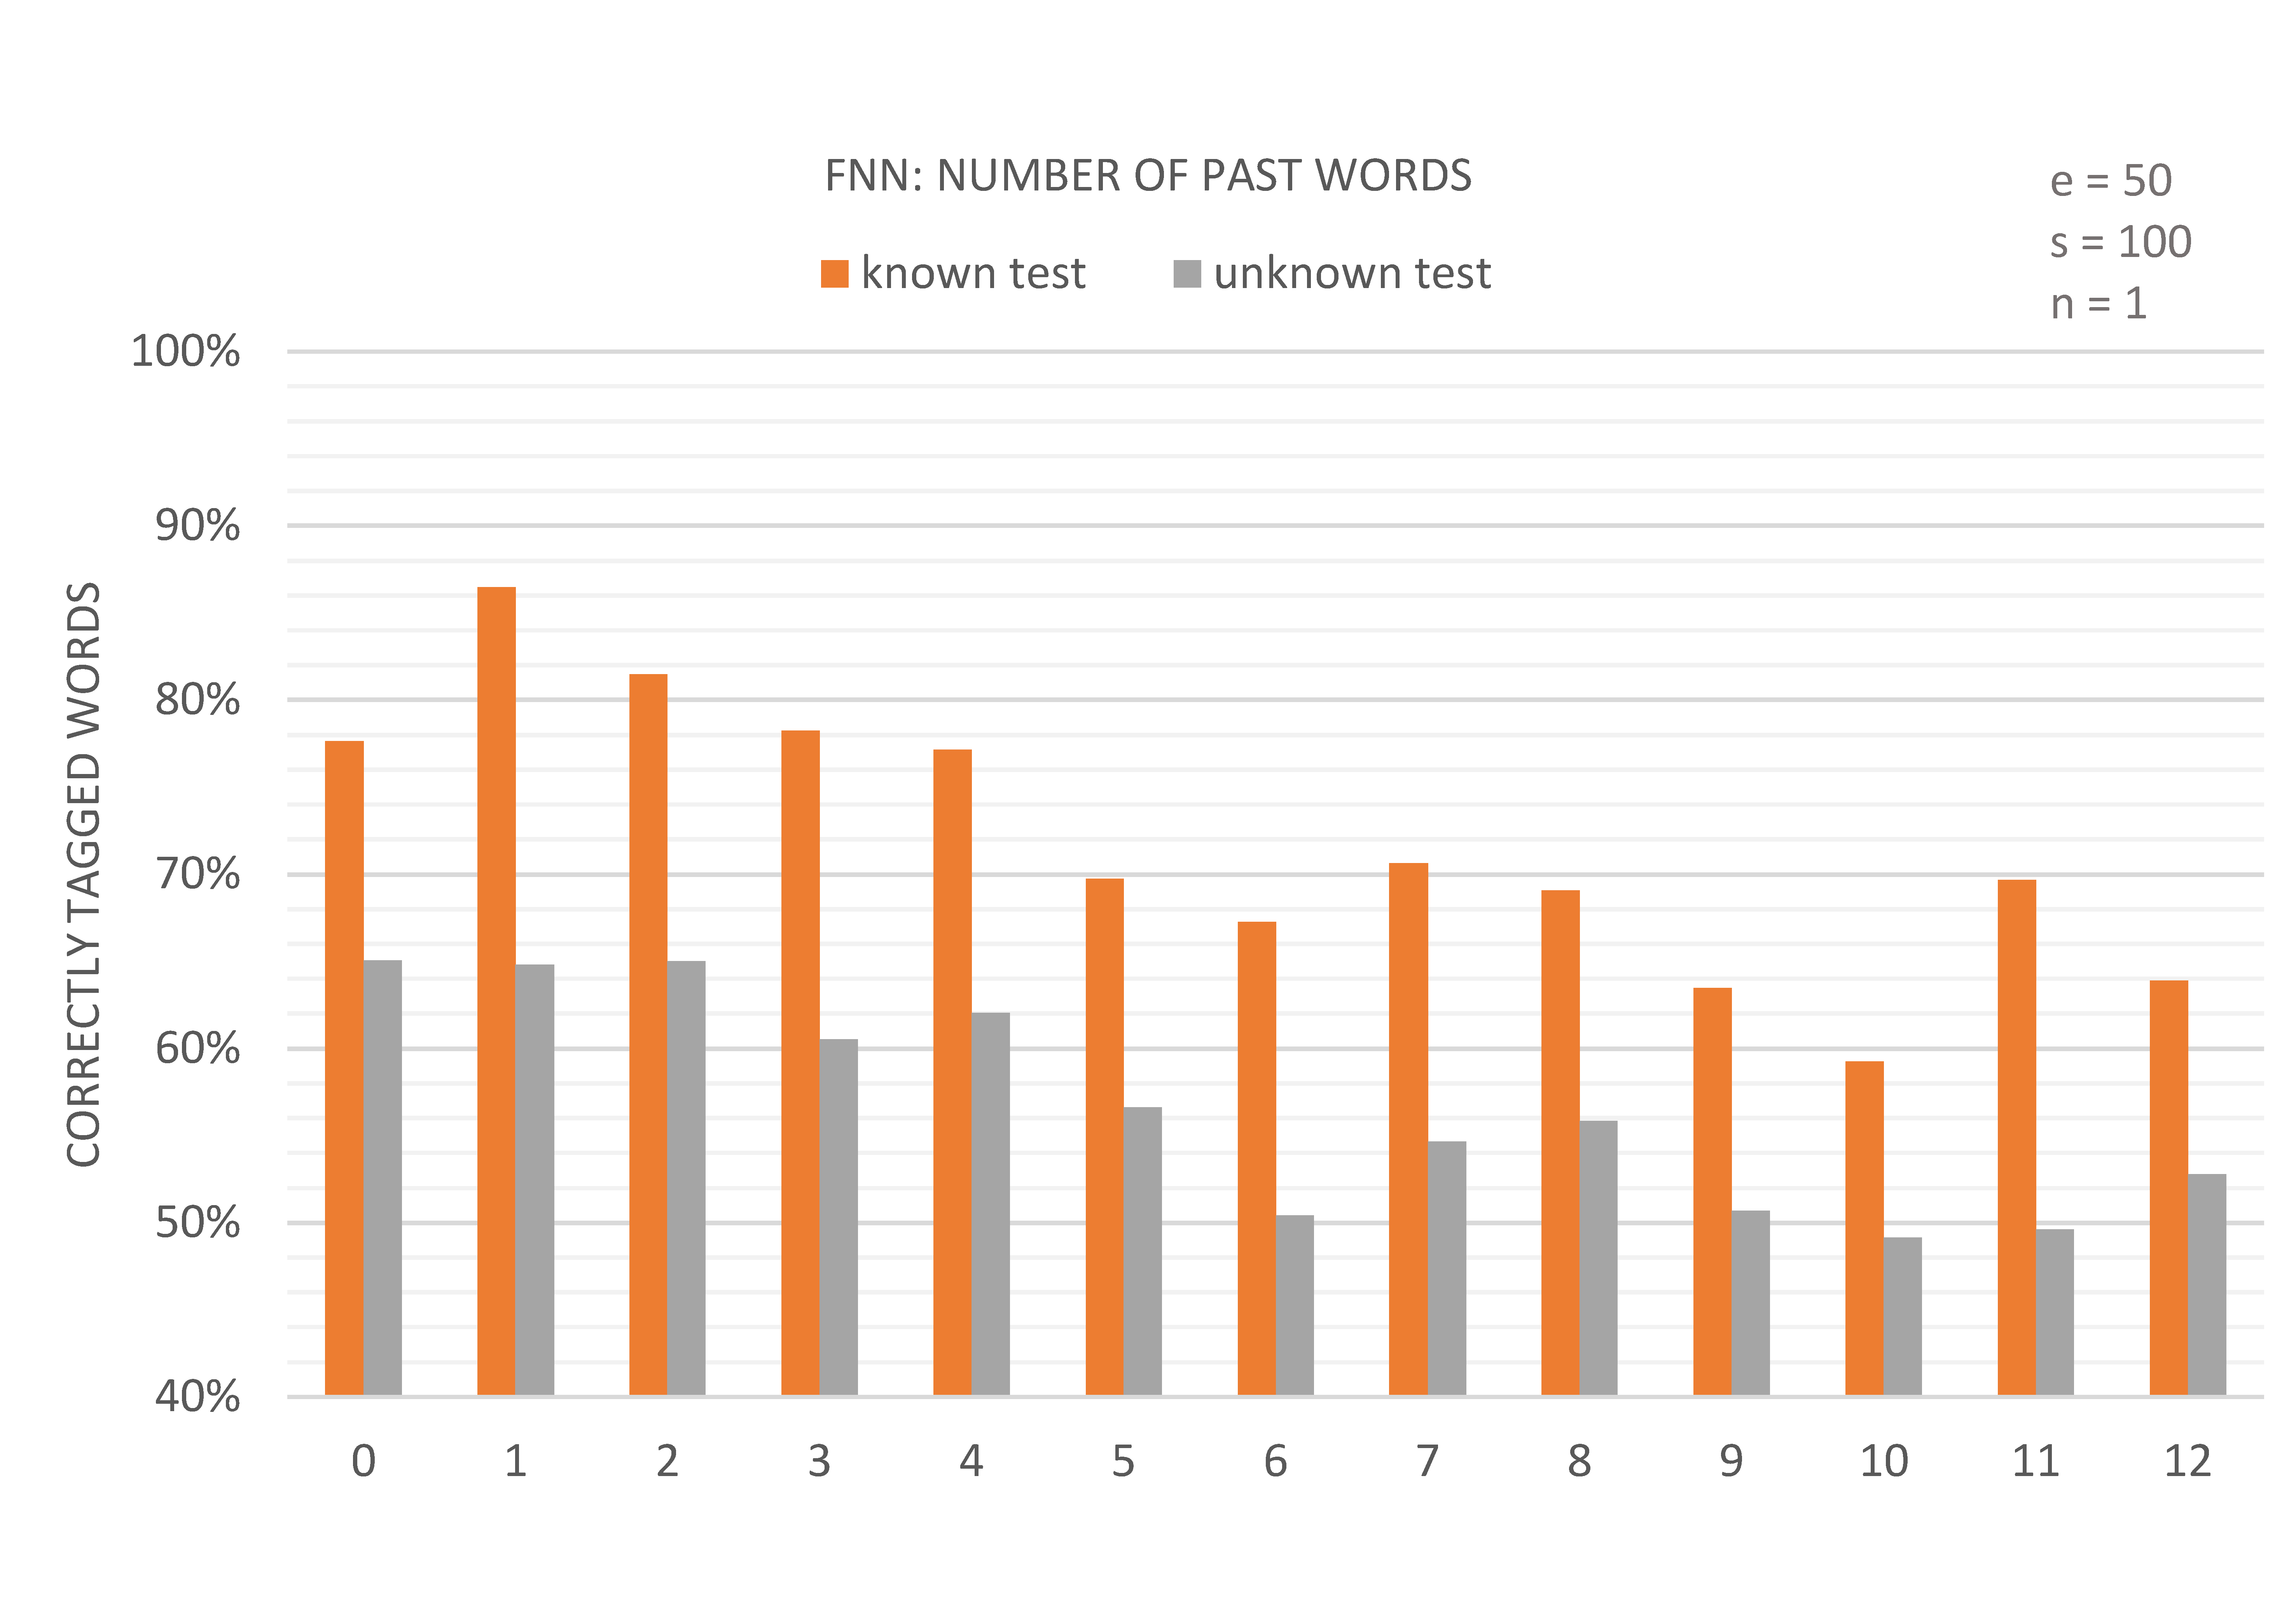
\includegraphics[width=1.07\textwidth]{images/evaluation_fnn_p}
	\caption[FNN Evaluation: Number of Past Words]{The evaluation results of the FNN for parameter $p$: the number of preceding words.}
	\label{f.evaluation.fnn.p}
\end{figure}

For the known test, the model with $p=1$ clearly achieves the highest accuracy with 86.1\% correctly tagged words. It also has the highest kappa score with $\kappa=0.802$. With more than one preceding word, the accuracy decreases. The best result (65.1\% accuracy and $\kappa=0.588$) for the unknown test was reached by the model trained without any preceding words at all. It should be noted, however, that the results of the two following models with 1 or 2 preceding words are almost as precise as the first one. With more than 2 preceding words, the accuracy decreases.

\b{Training group 2} included the evaluation based on 18 different values for the embedding size $e$ of the input words for the FNN. The results are presented in Figure \ref{f.evaluation.fnn.e}. With a few exceptions, the accuracy for the known test  increases slightly with larger embeddings, reaching a maximum of 90.5\% (and $\kappa=0.801$) on an embedding size of 600. The highest accuracy (70.1\%, $\kappa=0.639$) for the unknown test was reached by the model with an embedding size of 450.

\begin{figure}[H]
	\hspace{-5mm}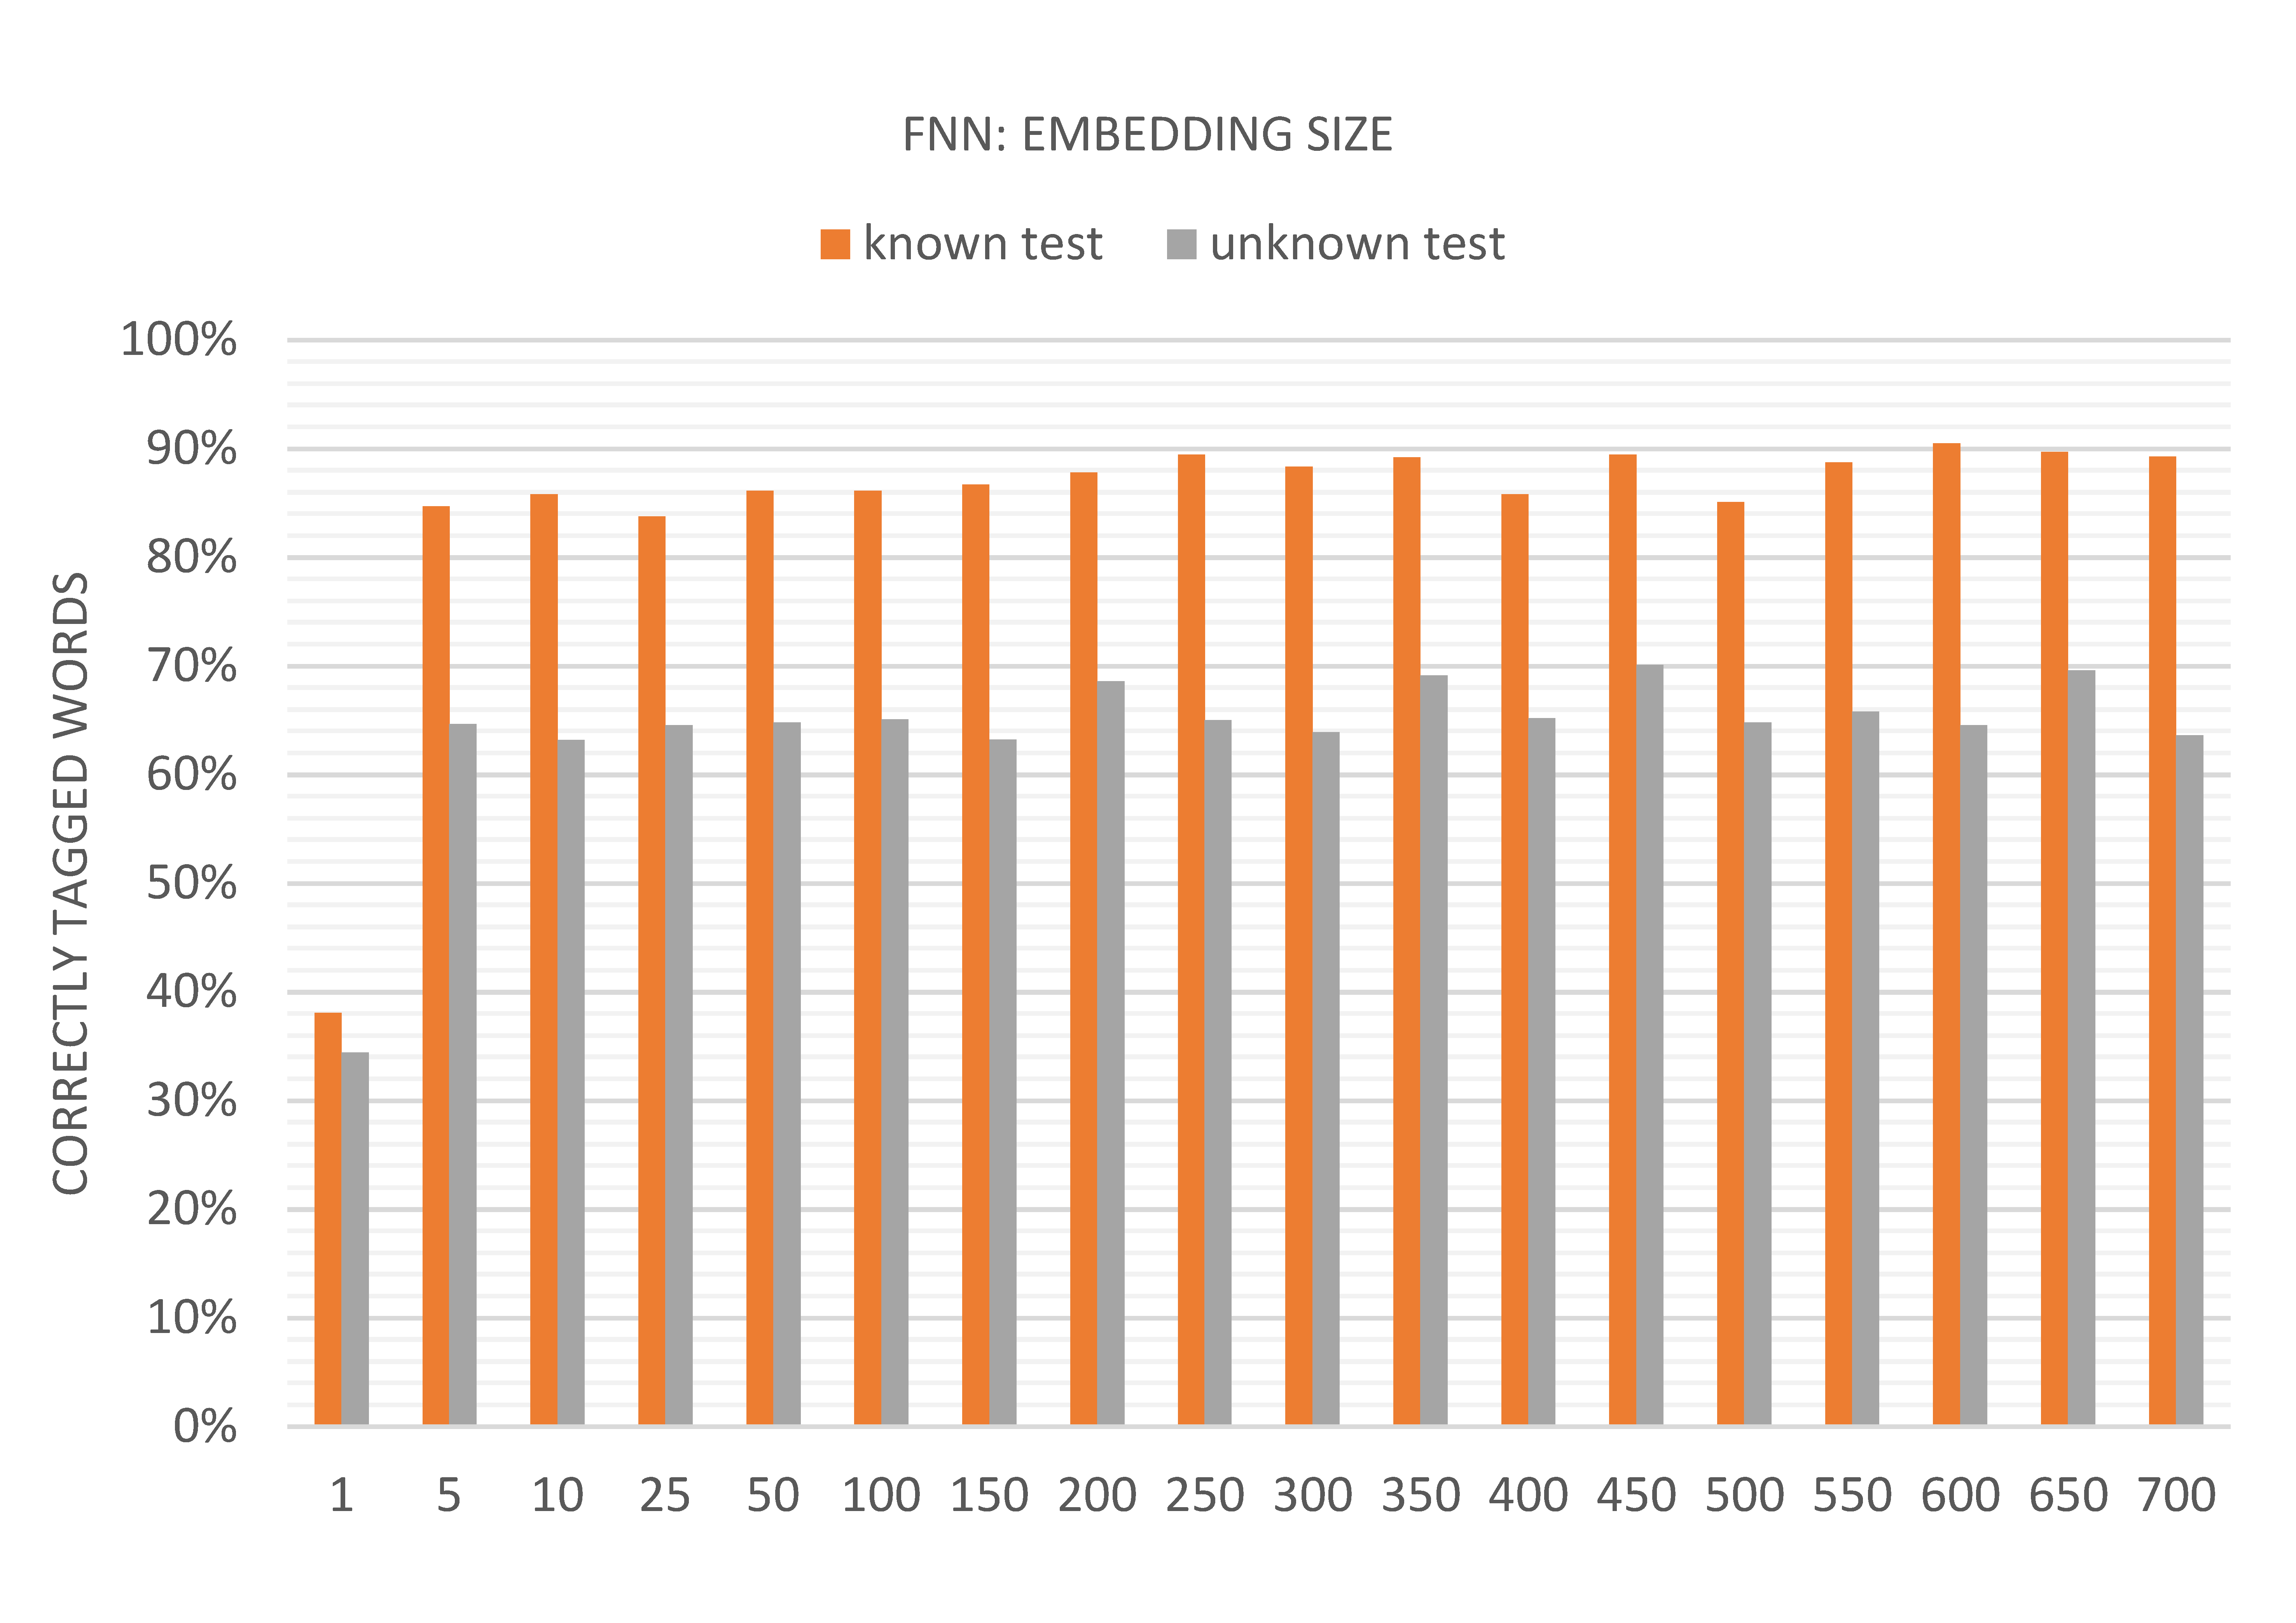
\includegraphics[width=1.07\textwidth]{images/evaluation_fnn_e}
	\caption[FNN Evaluation: Number of Past Words]{The evaluation results of the FNN for parameter $e$: the embedding size.}
	\label{f.evaluation.fnn.e}
\end{figure}

The results of the evaluation of \b{training group 3}, which varied the size of the hidden layer $s$, is illustrated in Figure \ref{f.evaluation.fnn.s}.

\begin{figure}[H]
	\hspace{-5mm}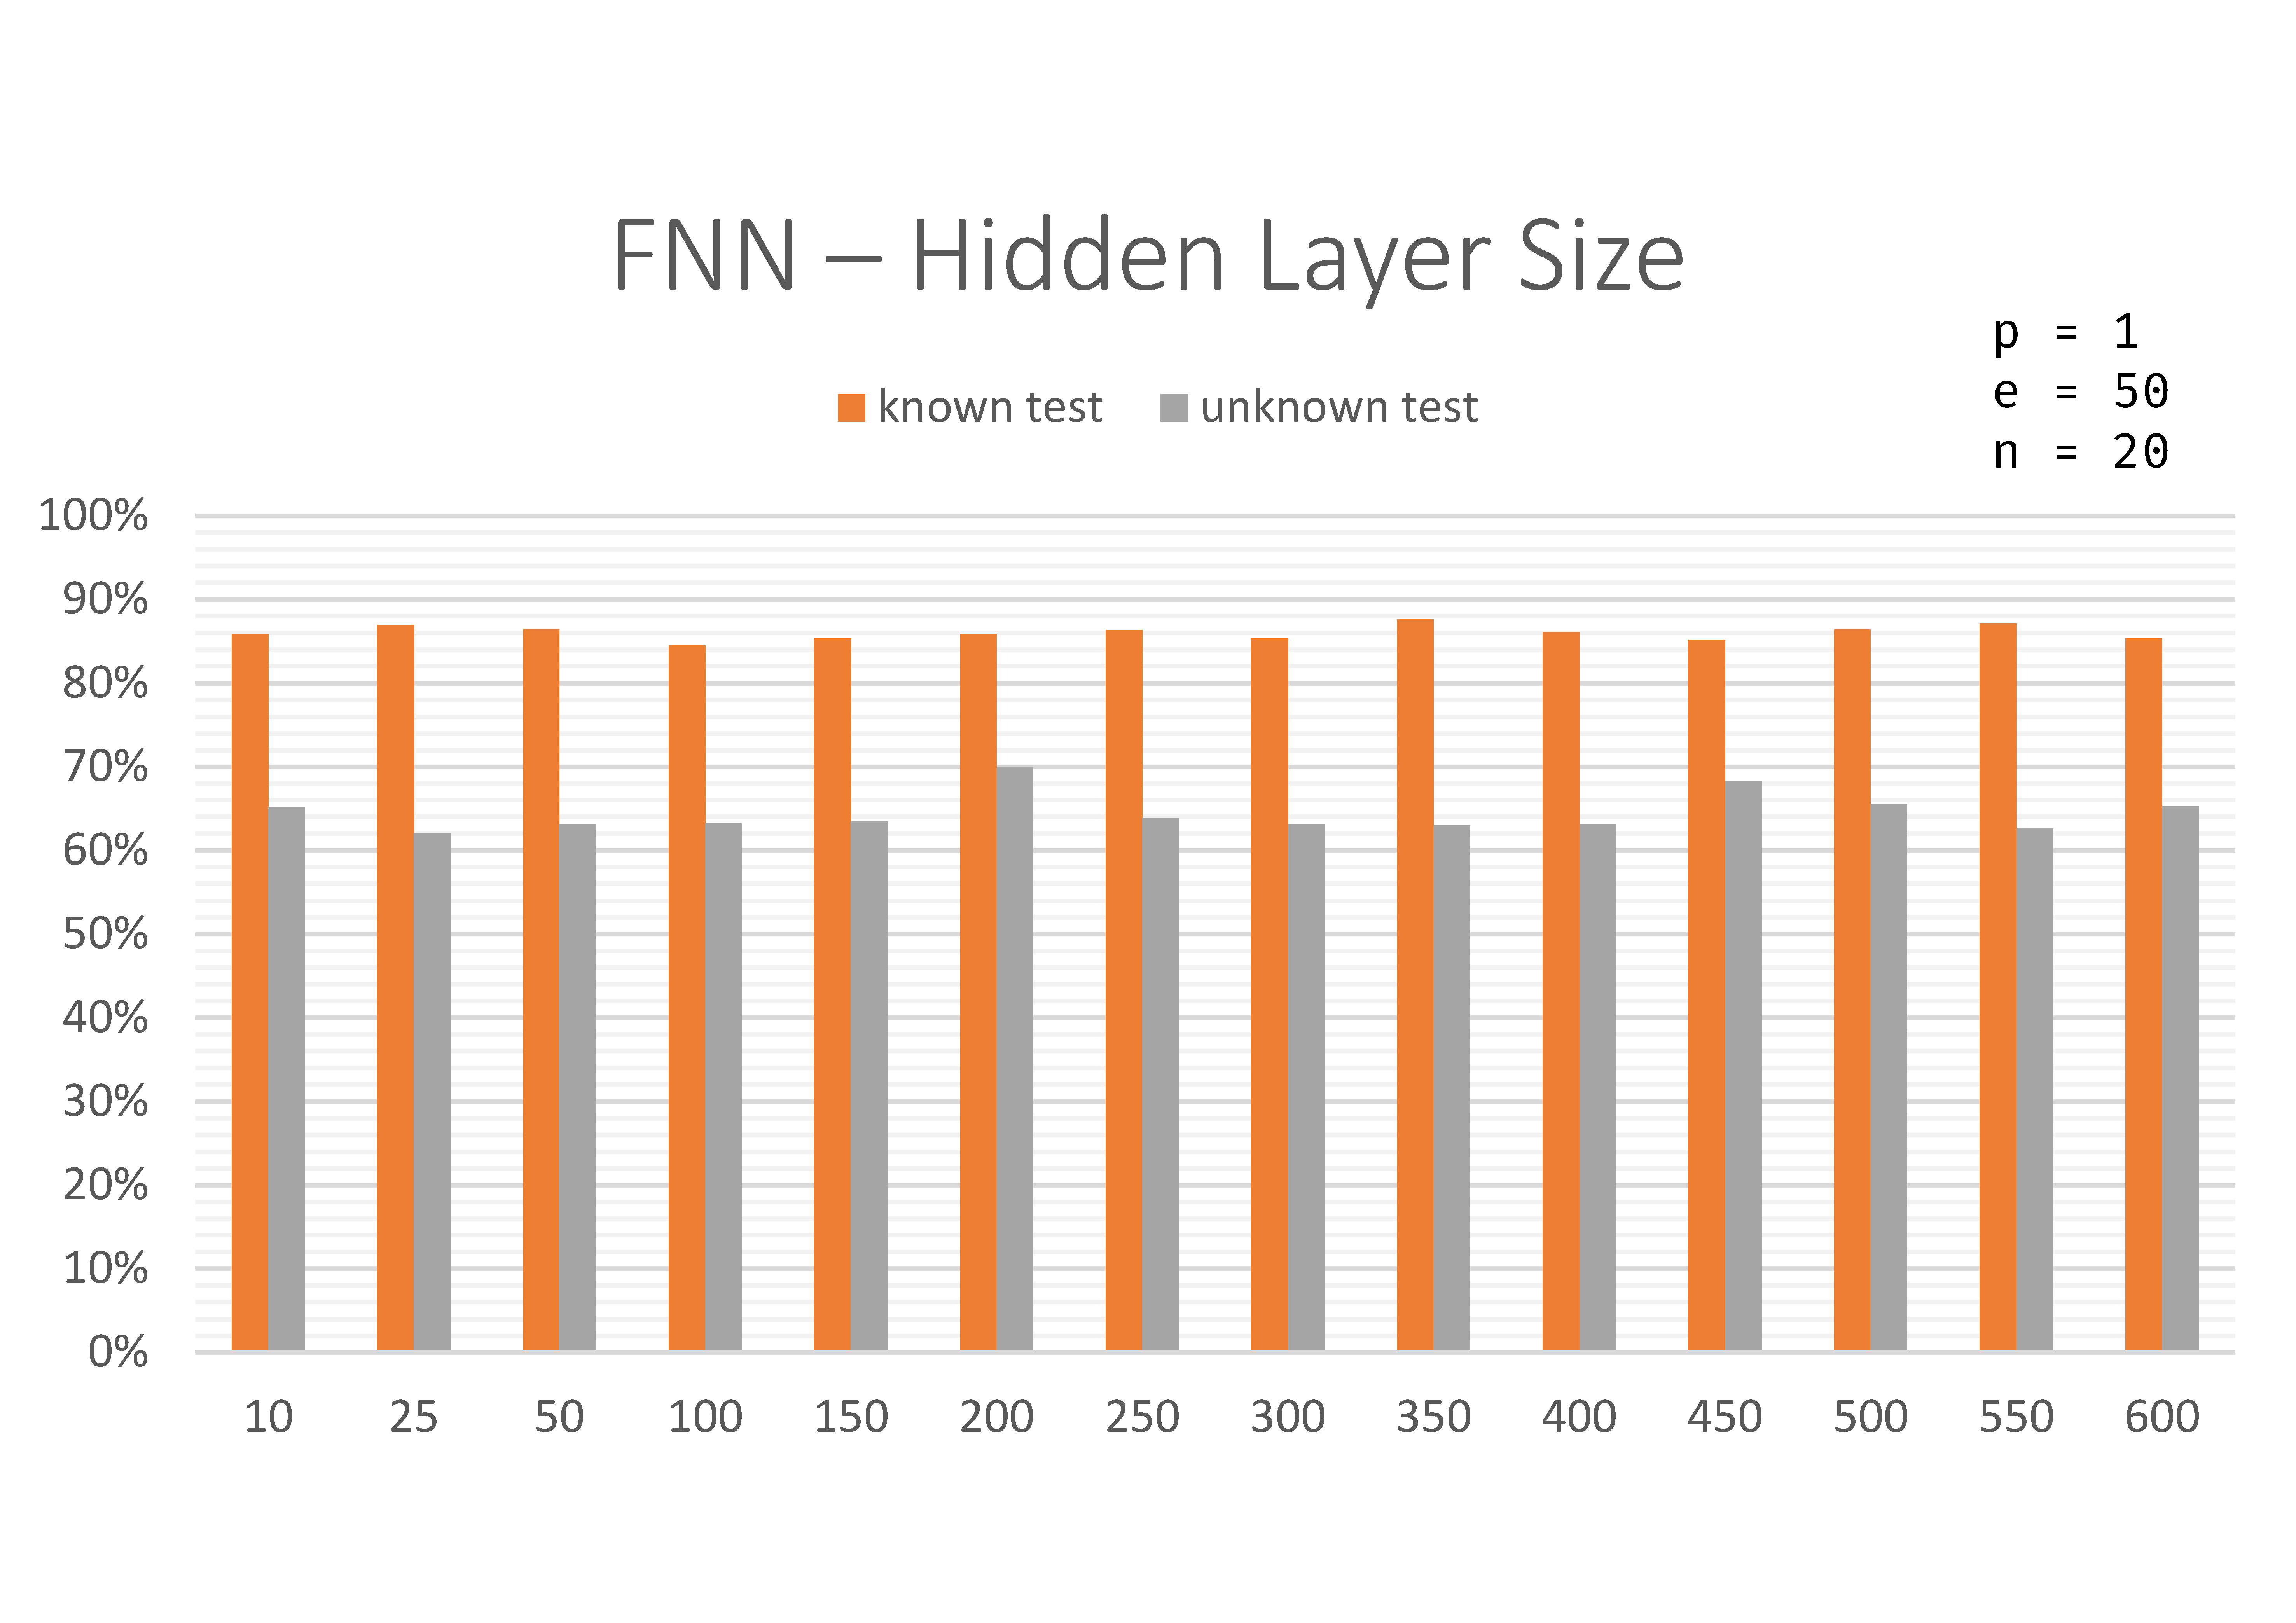
\includegraphics[width=1.07\textwidth]{images/evaluation_fnn_s}
	\caption[FNN Evaluation: Hidden Layer Size]{The evaluation results of the FNN for parameter $s$: the size of the hidden layer.}
	\label{f.evaluation.fnn.s}
\end{figure}

The highest accuracy of 89.1\% was achieved on the known test with a hidden layer size of 50 neurons, however, the highest kappa value $\kappa=0.813$ was assigned to a hidden layer size of 350. Although the accuracy of the models with $s<500$ seems to be slightly higher, no clear trend can be observed. The case is similar for the unknown test, except that models with $s>450$ have a higher, less fluctuating accuracy. The best result (71.5\%, $\kappa=0.643$) was reached by the model with $s=700$, however, the highest kappa value $\kappa=0.649$ was assigned to a hidden layer size of 450.

For \b{training group 4}, models were trained with different numbers of training epochs $n$. Figure \ref{f.evaluation.fnn.n} presents the results.

\begin{figure}[H]
	\hspace{-5mm}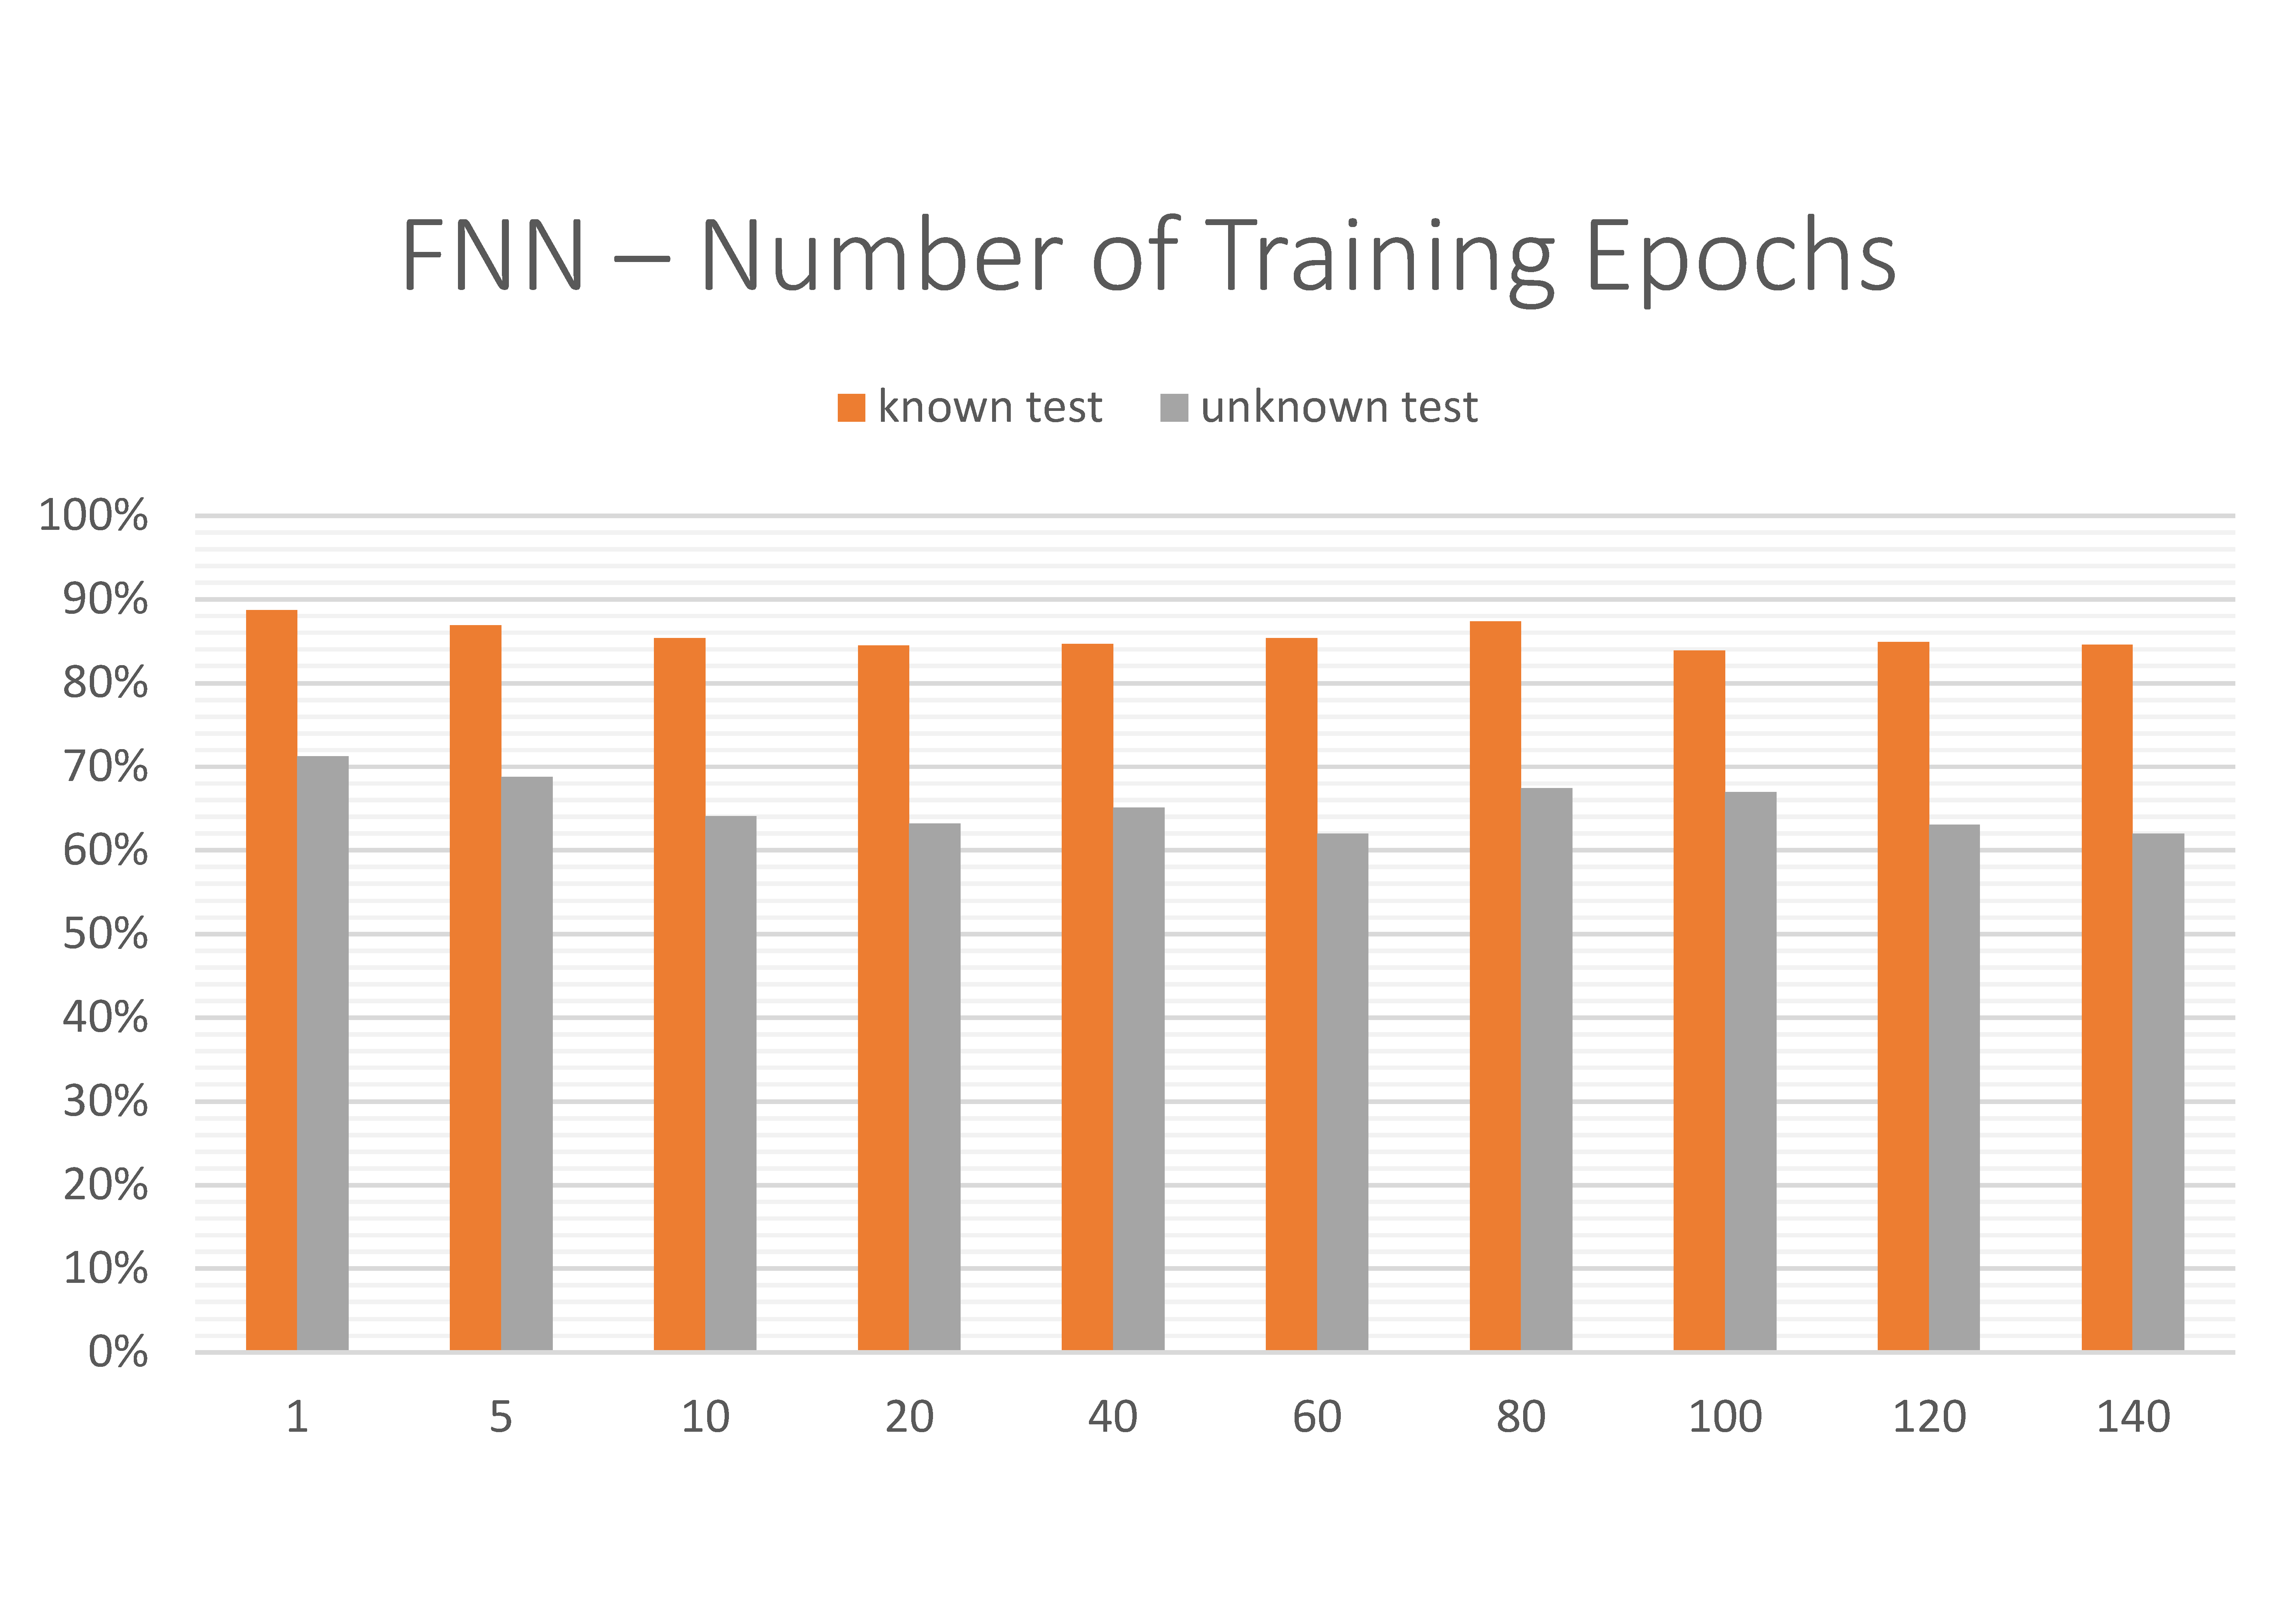
\includegraphics[width=1.07\textwidth]{images/evaluation_fnn_n}
	\caption[FNN Evaluation: Number of Training Epochs]{The evaluation results of the FNN for parameter $n$: the number of training epochs.}
	\label{f.evaluation.fnn.n}
\end{figure}

Overall, all models of the different training epochs achieved similar results on the known test without a discernible tendency. However, the model with $n=80$ stands out slightly, with the highest accuracy of 87.7\% and the second highest $\kappa=0.808$. For the unknown test, the model with only 5 training epochs achieved a maximum accuracy of 68.8\% and $\kappa=0.622$.

Similar to training group 2, \b{training group 5} refers to the embedding size $e$, but utilizing a larger hidden layer size ($s=350$). The results are presented in Figure {\ref{f.evaluation.fnn.e2}}.

\begin{figure}[H]
	\hspace{-5mm}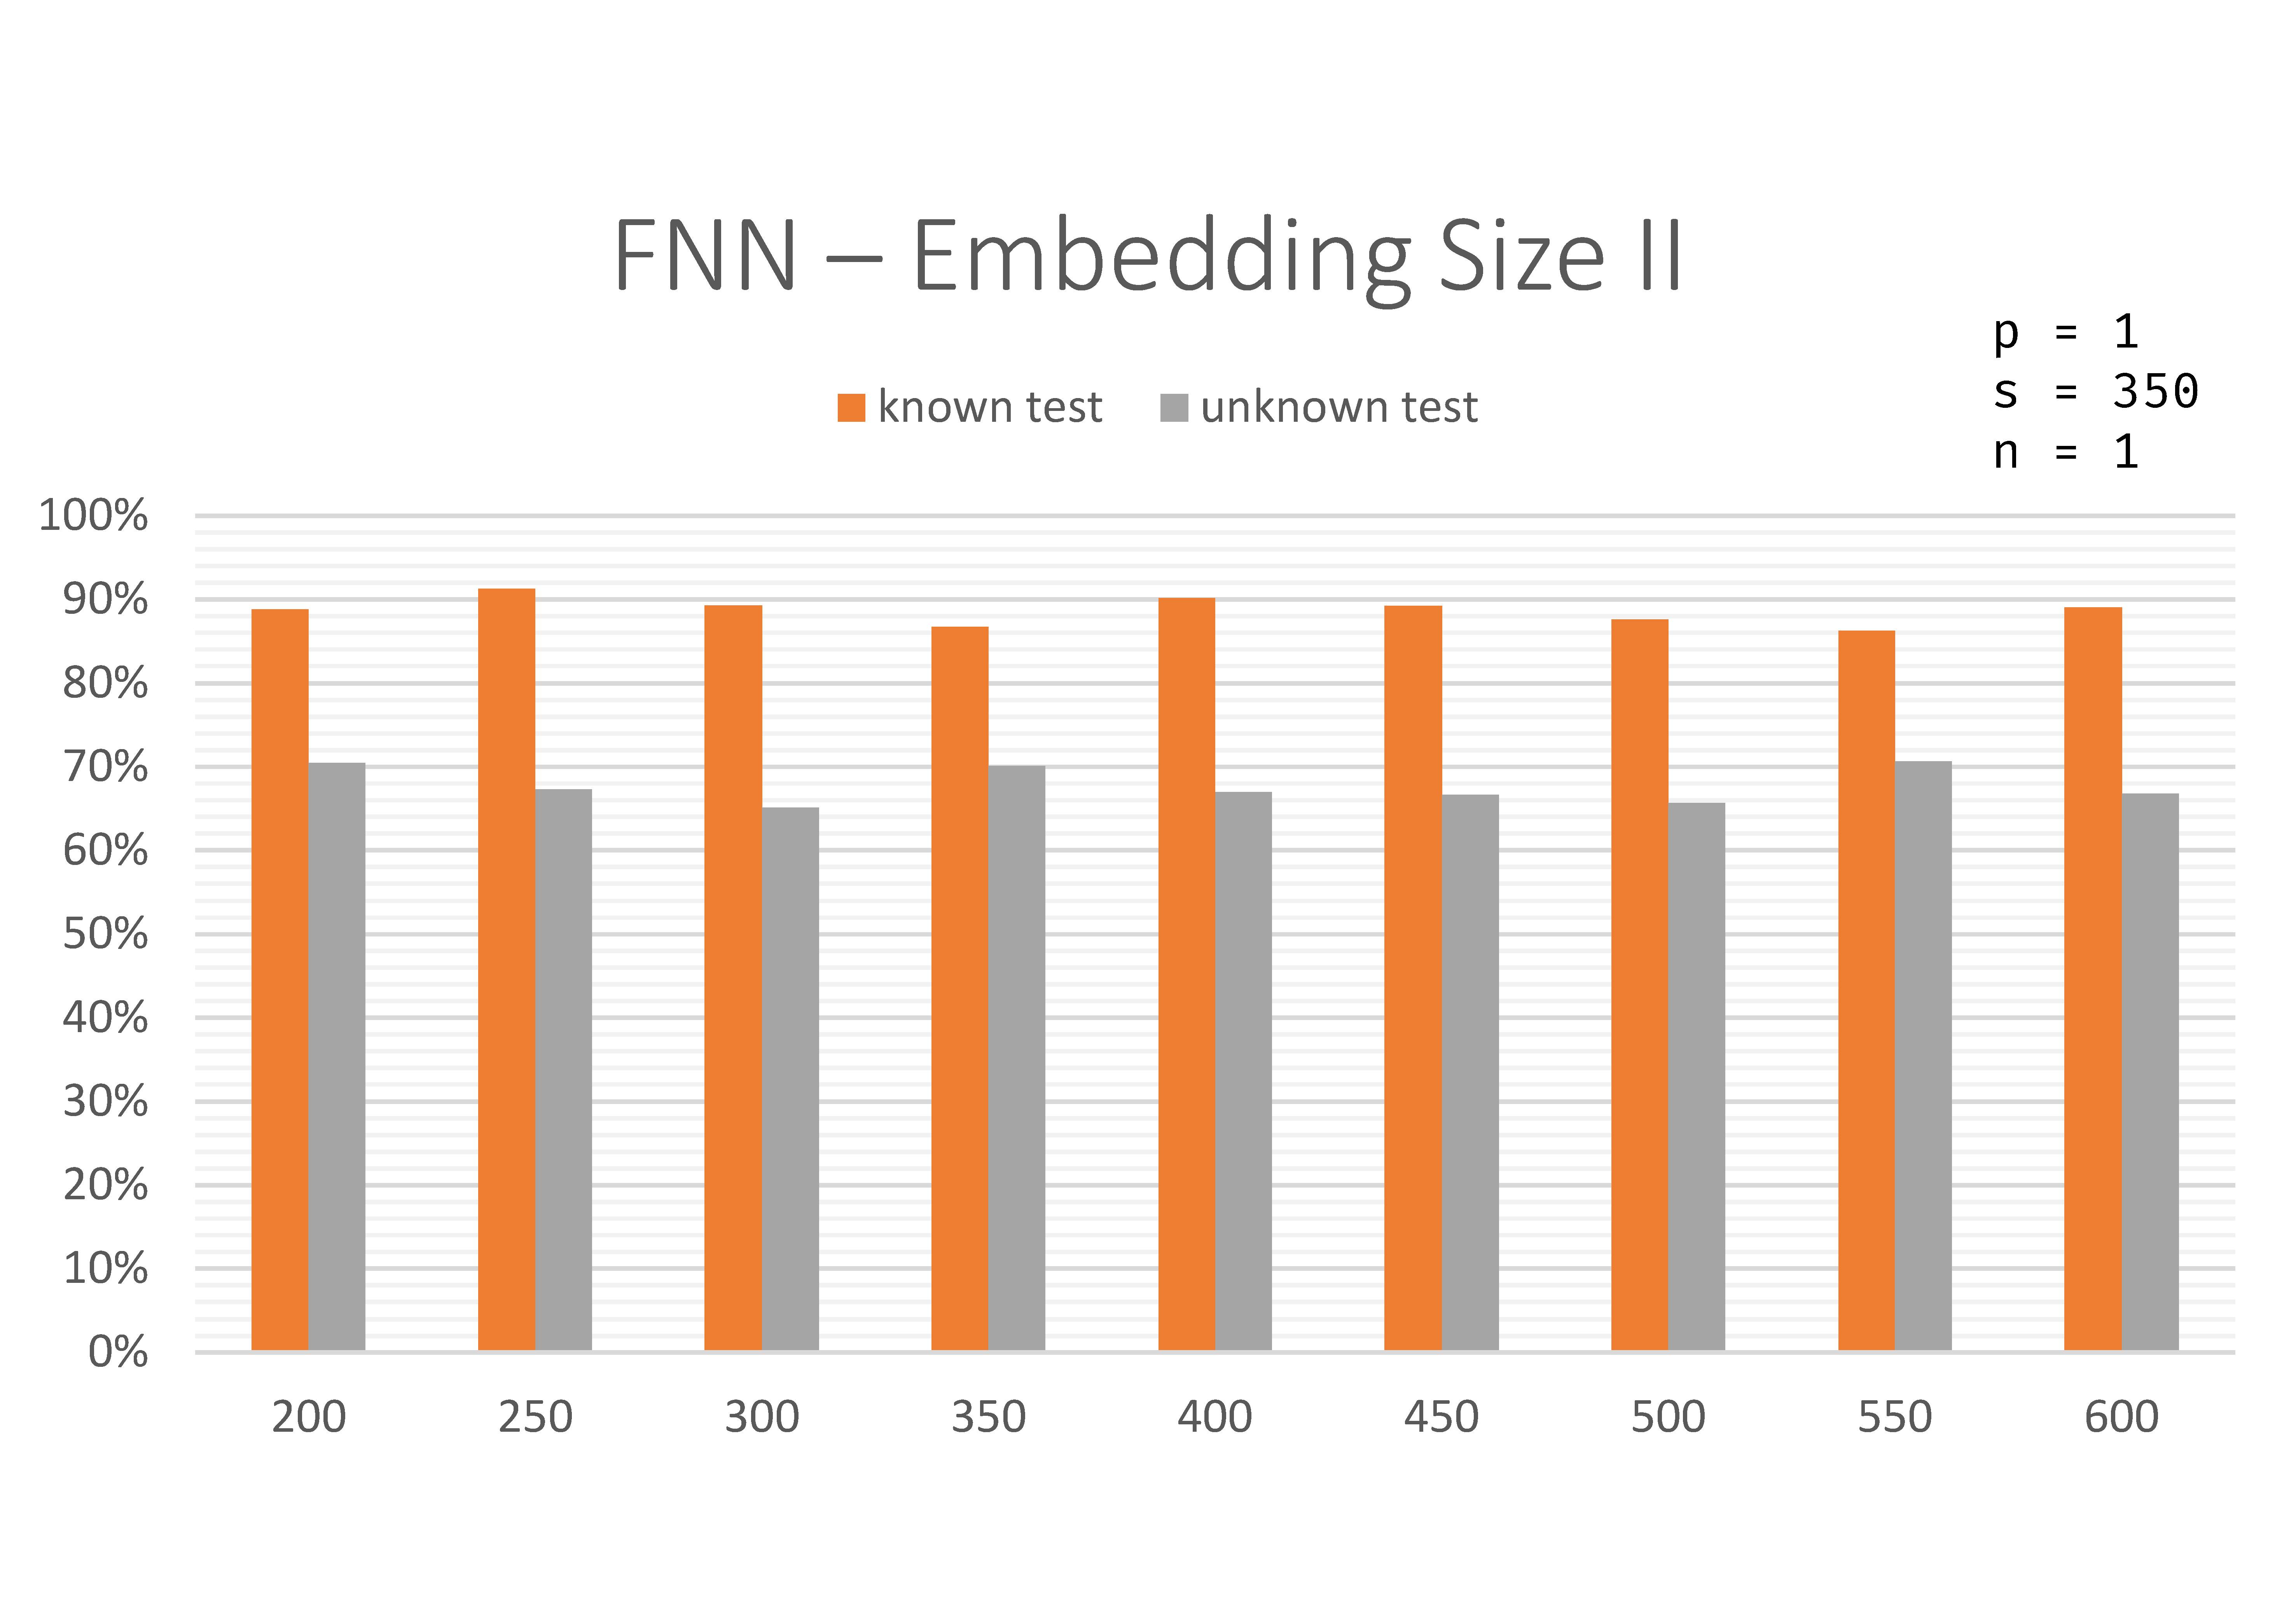
\includegraphics[width=1.07\textwidth]{images/evaluation_fnn_e2}
	\caption[FNN Evaluation: Embedding Size II]{The evaluation results of the FNN for the embedding size $e$ with a larger hidden layer size $s=350$.}
	\label{f.evaluation.fnn.e2}
\end{figure}

Compared to training group 2, the results were slightly better. Evaluating the known test, the highest accuracy of 91.4\% ($\kappa=0.807$) was reached by a model with embedding size $e=250$. Nevertheless, the highest kappa value $\kappa=0.818$ was assigned to the model with $e=500$, which achieved a lower accuracy of 87.8\%. For the unknown test, the model with $e=550$ tagged the most words correctly (70.7\%, $\kappa=0.640$).

Similar to training group 3, \b{training group 6} refers to the hidden layer size $s$, with the difference of using a larger embedding size ($e=250$). Figure {\ref{f.evaluation.fnn.s2}} presents the results.

\begin{figure}[H]
	\hspace{-5mm}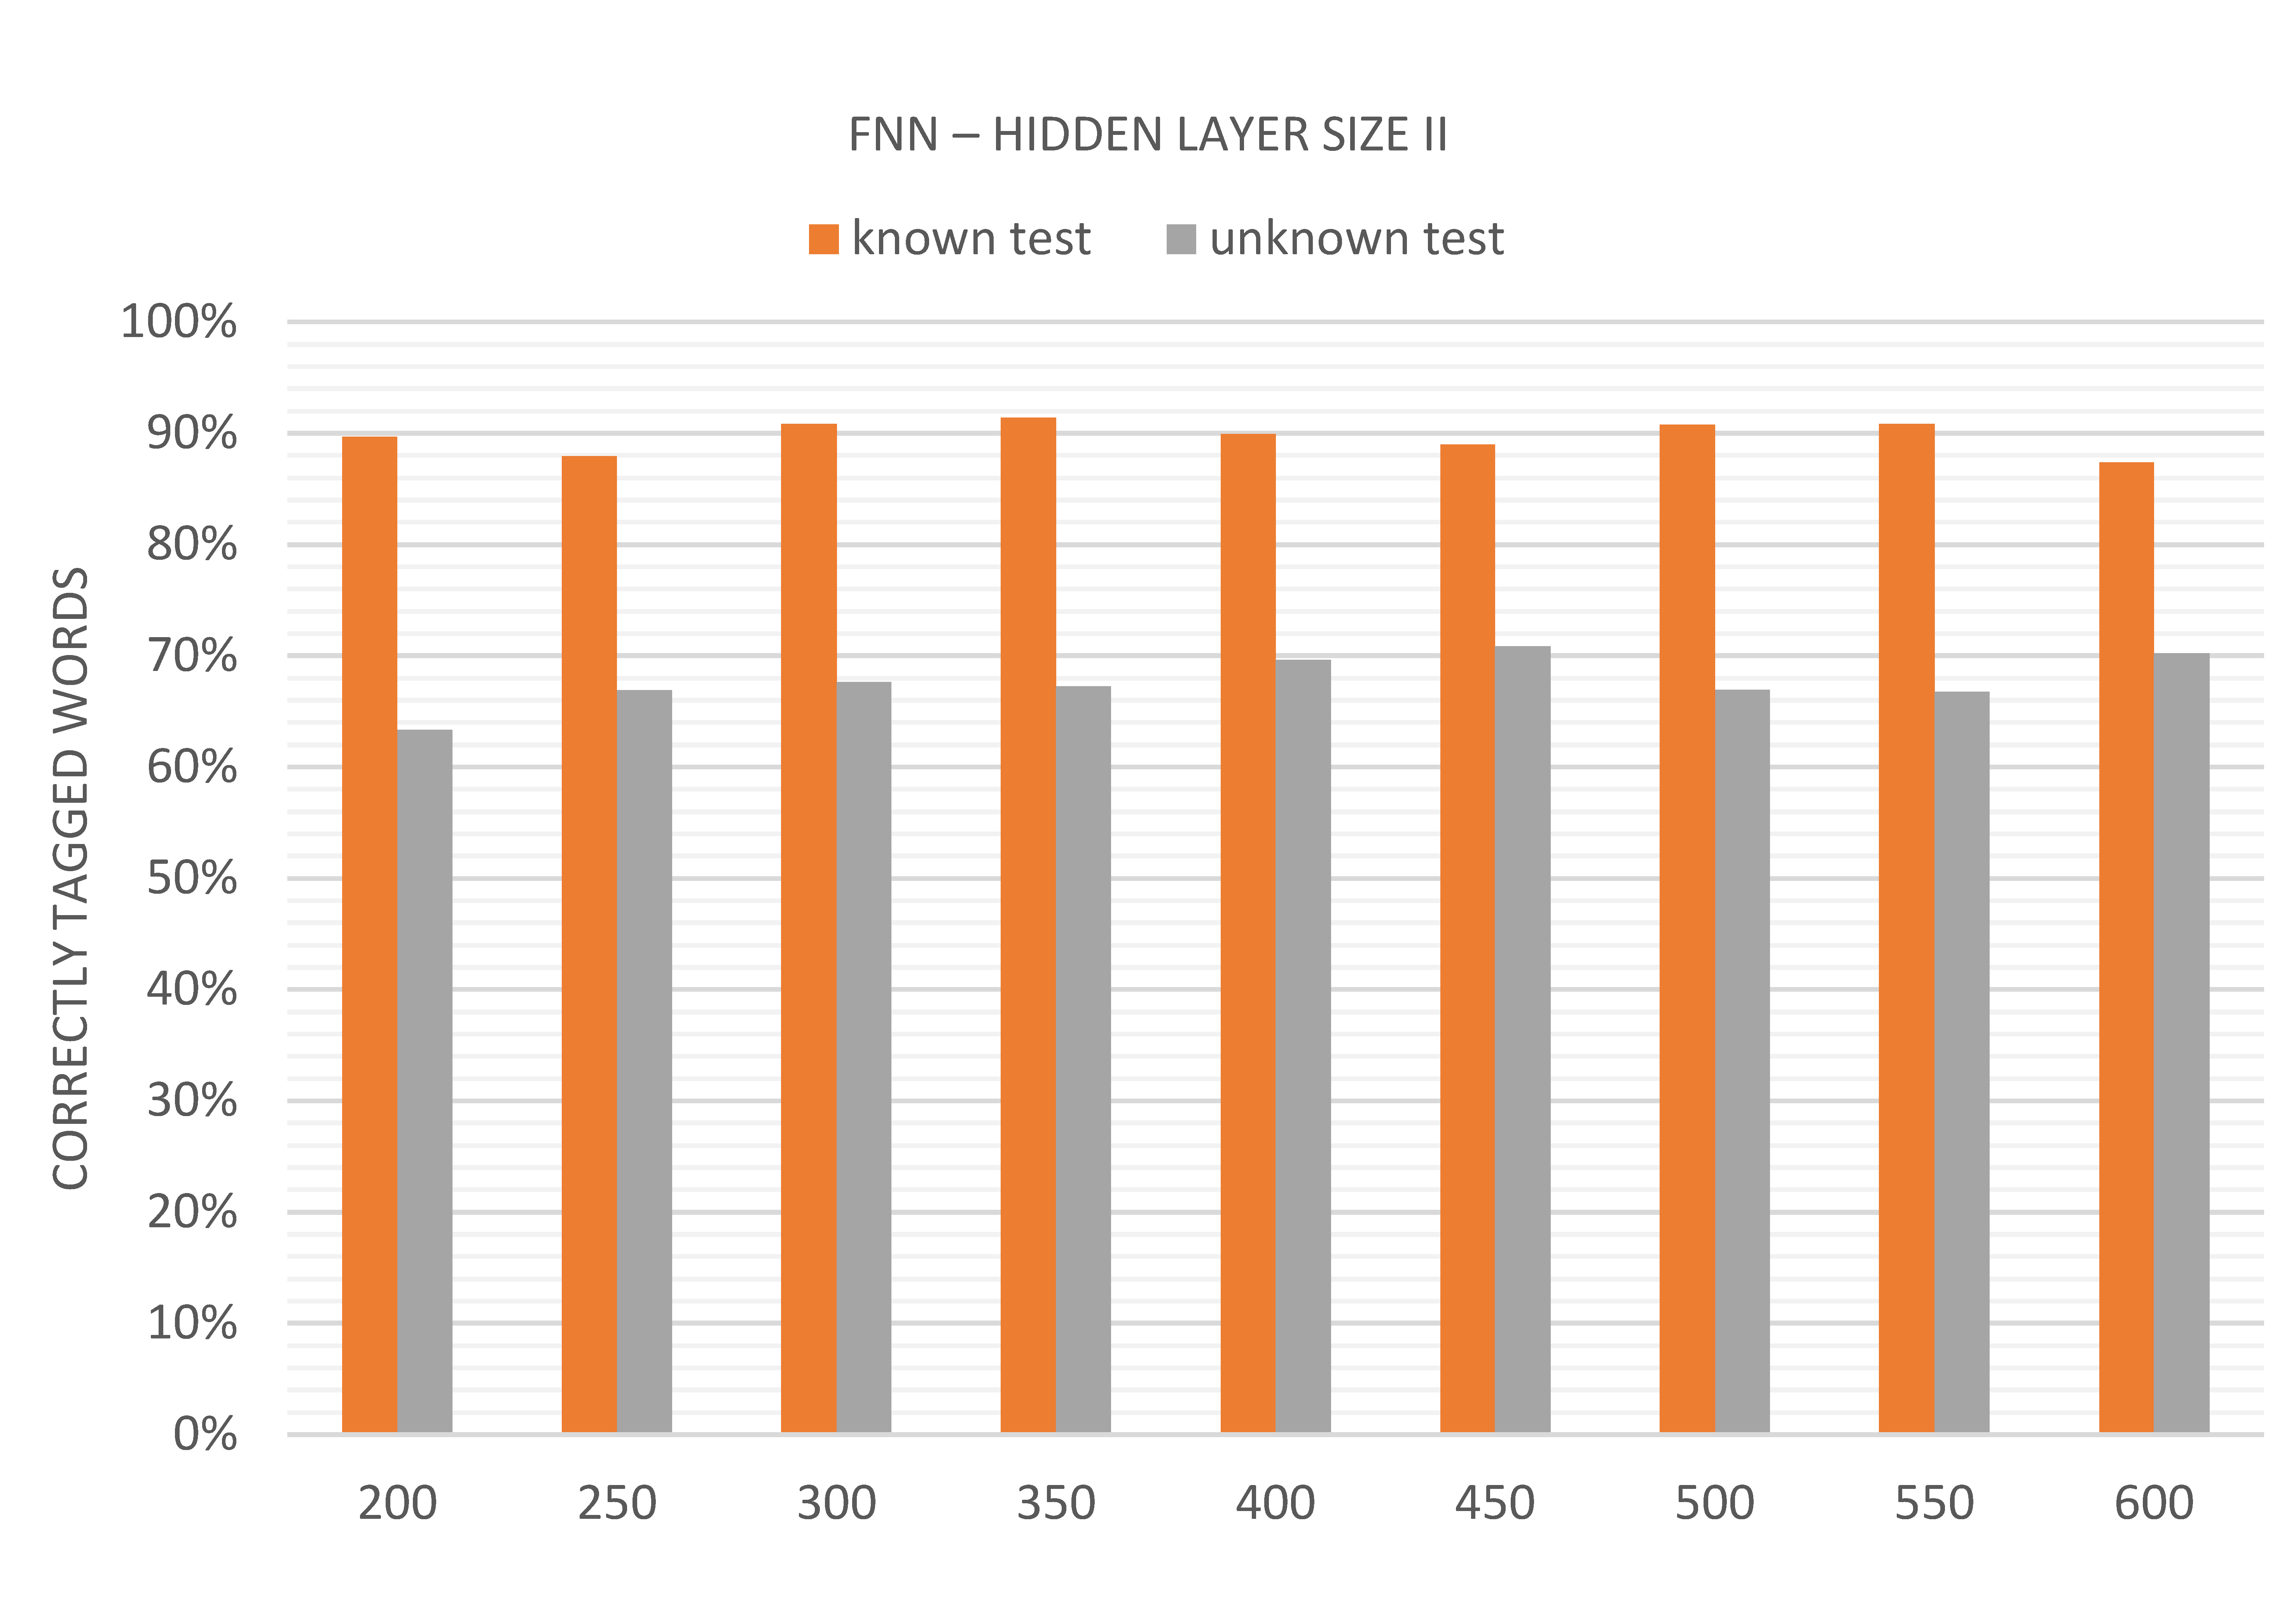
\includegraphics[width=1.07\textwidth]{images/evaluation_fnn_s2}
	\caption[FNN Evaluation: Hidden Layer Size II]{The evaluation results of the FNN for the hidden layer size $s$ with a larger embedding size $e=250$.}
	\label{f.evaluation.fnn.s2}
\end{figure}

This parameter configuration performed slightly better for both tests comparing to training group 3. Evaluating the known test, the highest accuracy of 91.4\% ($\kappa=0.807$) was again reached by the model with hidden layer size $s=350$. Nevertheless, the highest kappa value $\kappa=0.821$ was assigned to the model with $s=500$, which achieved a slightly lower accuracy of 90.8\%. For the unknown test, the model with $s=450$ tagged the most words correctly (70.9\%, $\kappa=0.643$).

\b{Training group 7} increases the size of the whole network by enlarging the embedding size $e$ and the hidden layer size $s$ at the same time (combined to parameter $es$. The results are presented in Figure \ref{f.evaluation.fnn.es}. The value on the horizontal axis represents both, the embedding size and the hidden layer size.

\begin{figure}[H]
	\hspace{-5mm}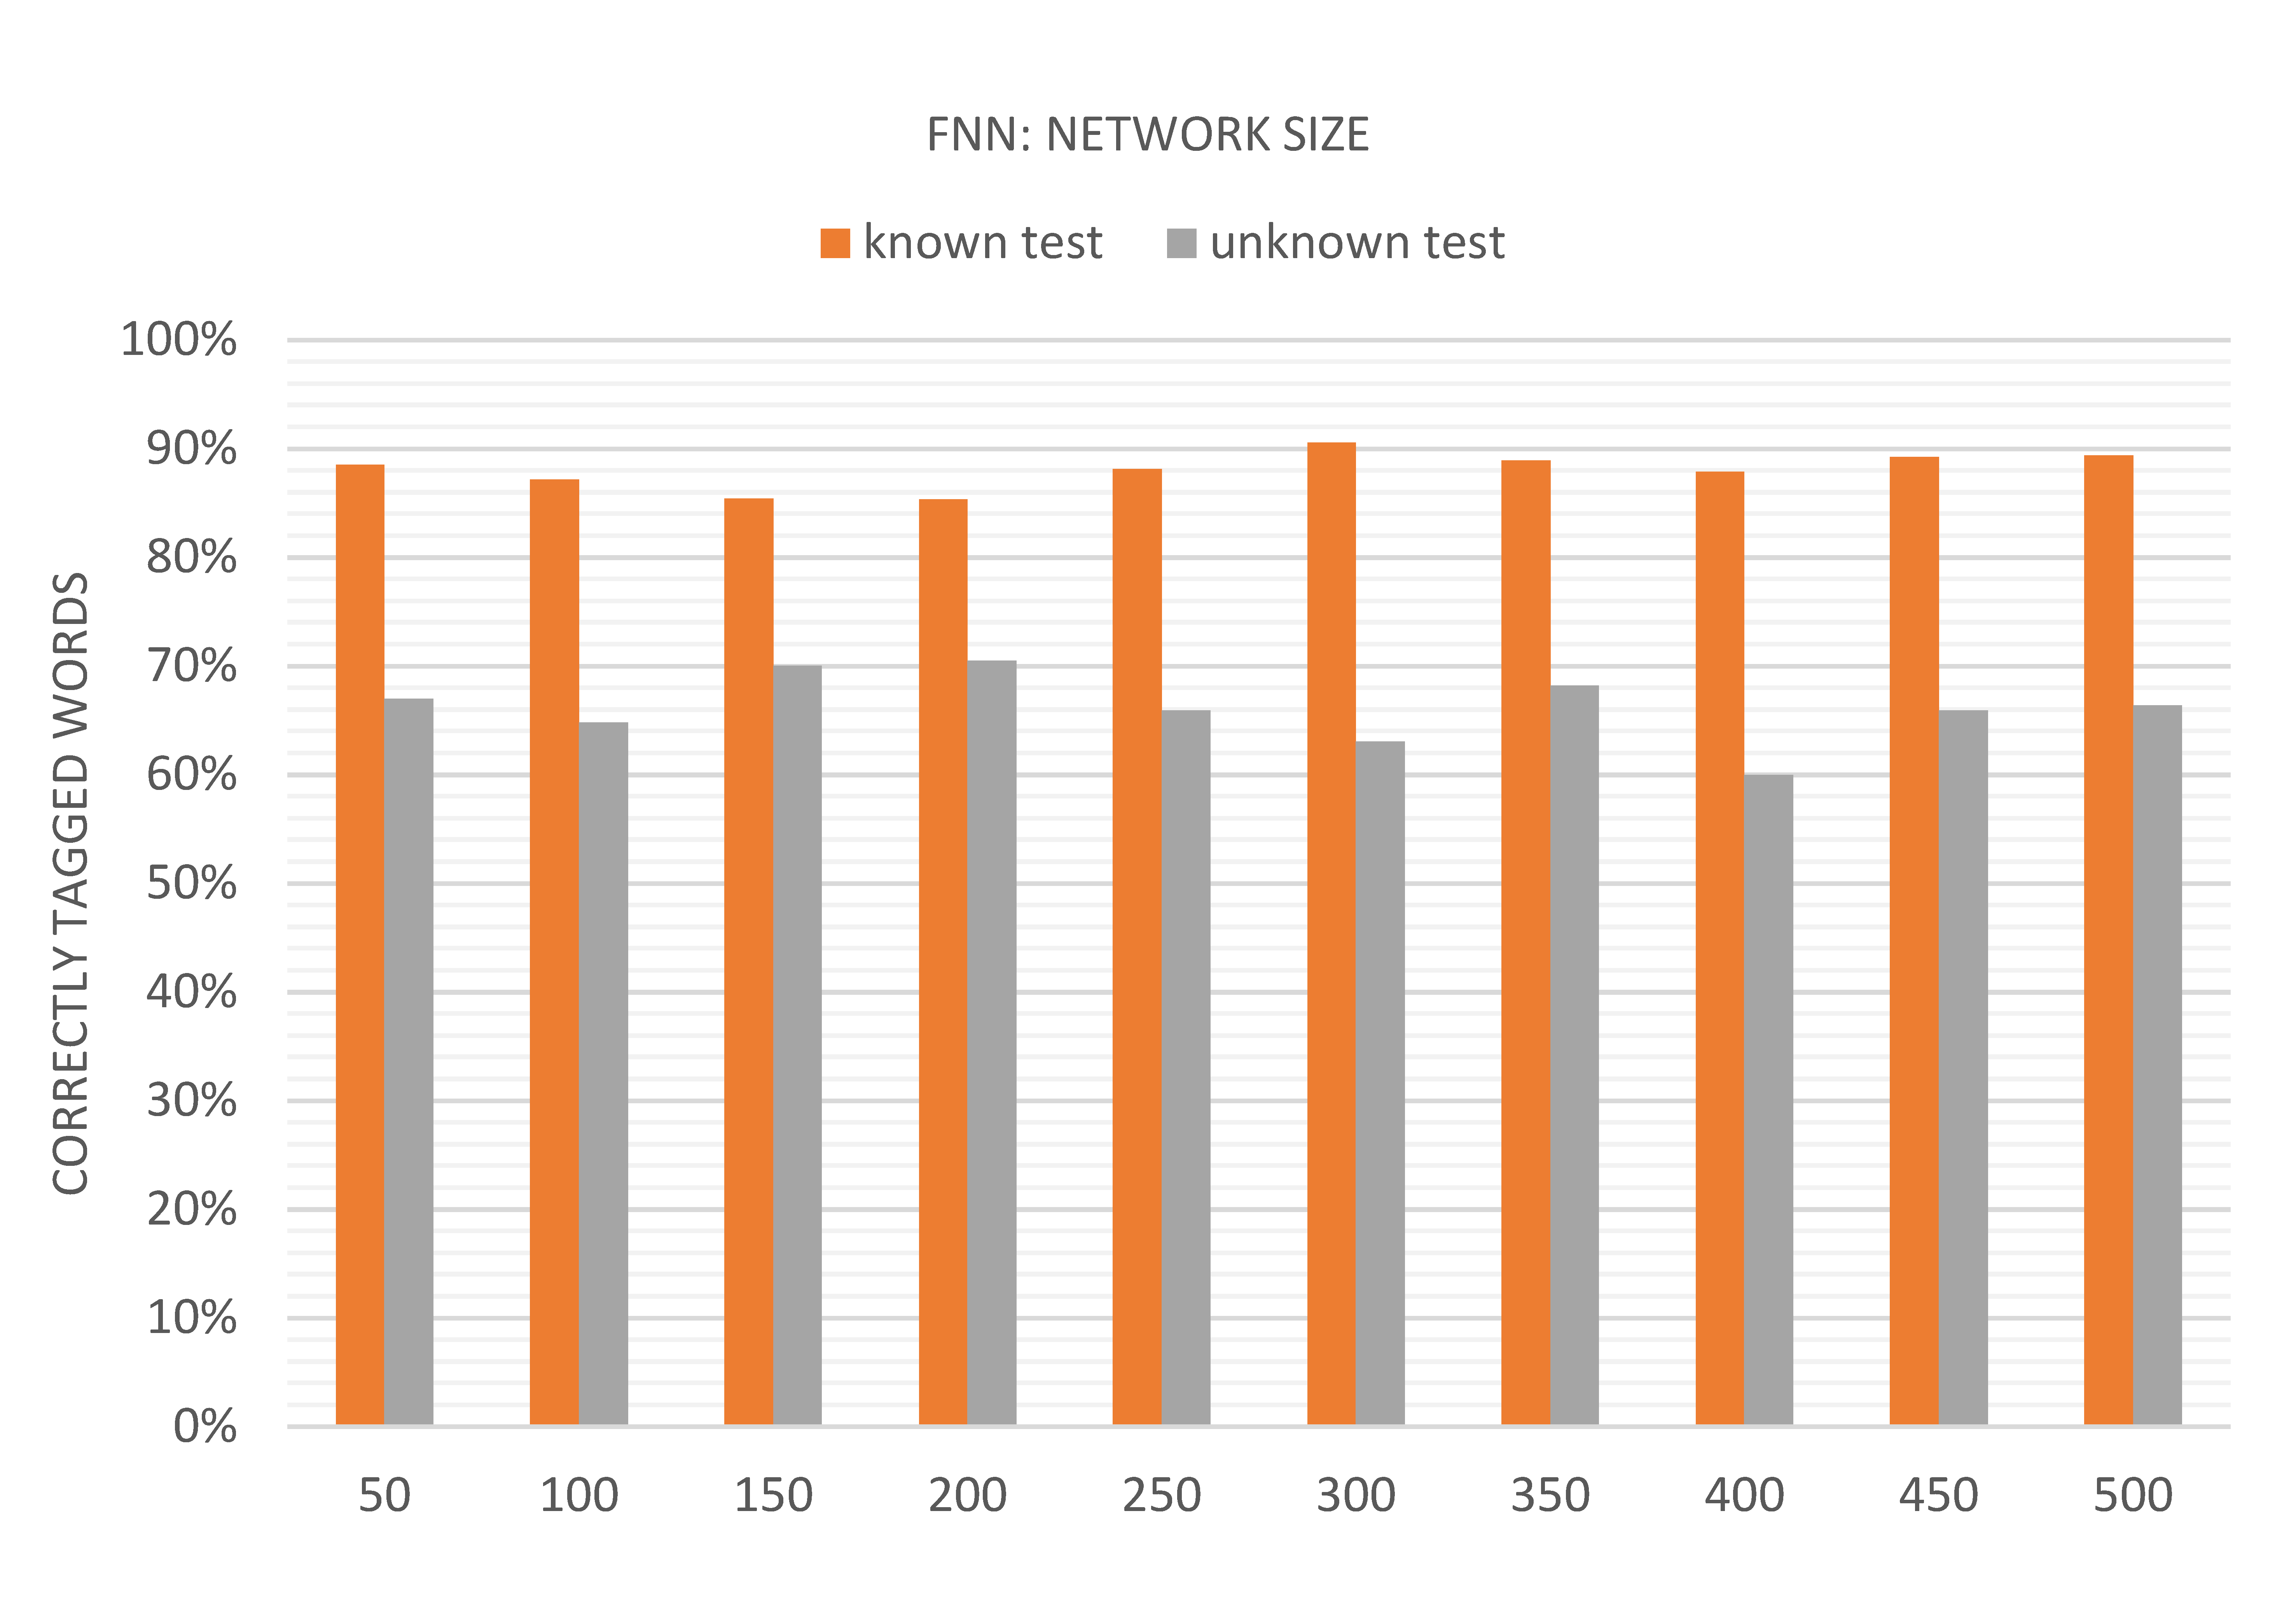
\includegraphics[width=1.07\textwidth]{images/evaluation_fnn_es}
	\caption[FNN Evaluation: Network Size]{The evaluation results of the FNN for enlarging the whole network by increasing the embedding size $e$ and the hidden layer size $s$ at the same time.}
	\label{f.evaluation.fnn.es}
\end{figure}

The highest accuracy of 90.6\% ($\kappa=0.802$) was achieved by the model with $es=300$ for the known test, however the highest kappa value $\kappa=0.809$ was assigned to a dimension of $es=500$. The best result for the unknown test was reached by $es=200$ with an accuracy of 70.5\% and $\kappa=0.639$.

The last training group for the FNN, \b{training group 8}, refers to parameter $a$: the activation function (all activation functions used for training were introduced in Chapter \ref{c.postagging.fnn.architecture}). The accuracy results of 8 models that were trained with different activation function each is presented in Figure \ref{f.evaluation.fnn.a}. The configuration of the other training parameters was based on the results of the preceding training groups, using $t=1$, $e=250$ and $s=350$. The number of training epochs was chosen with respect to a reasonable training time.

\begin{figure}[H]
	\hspace{-5mm}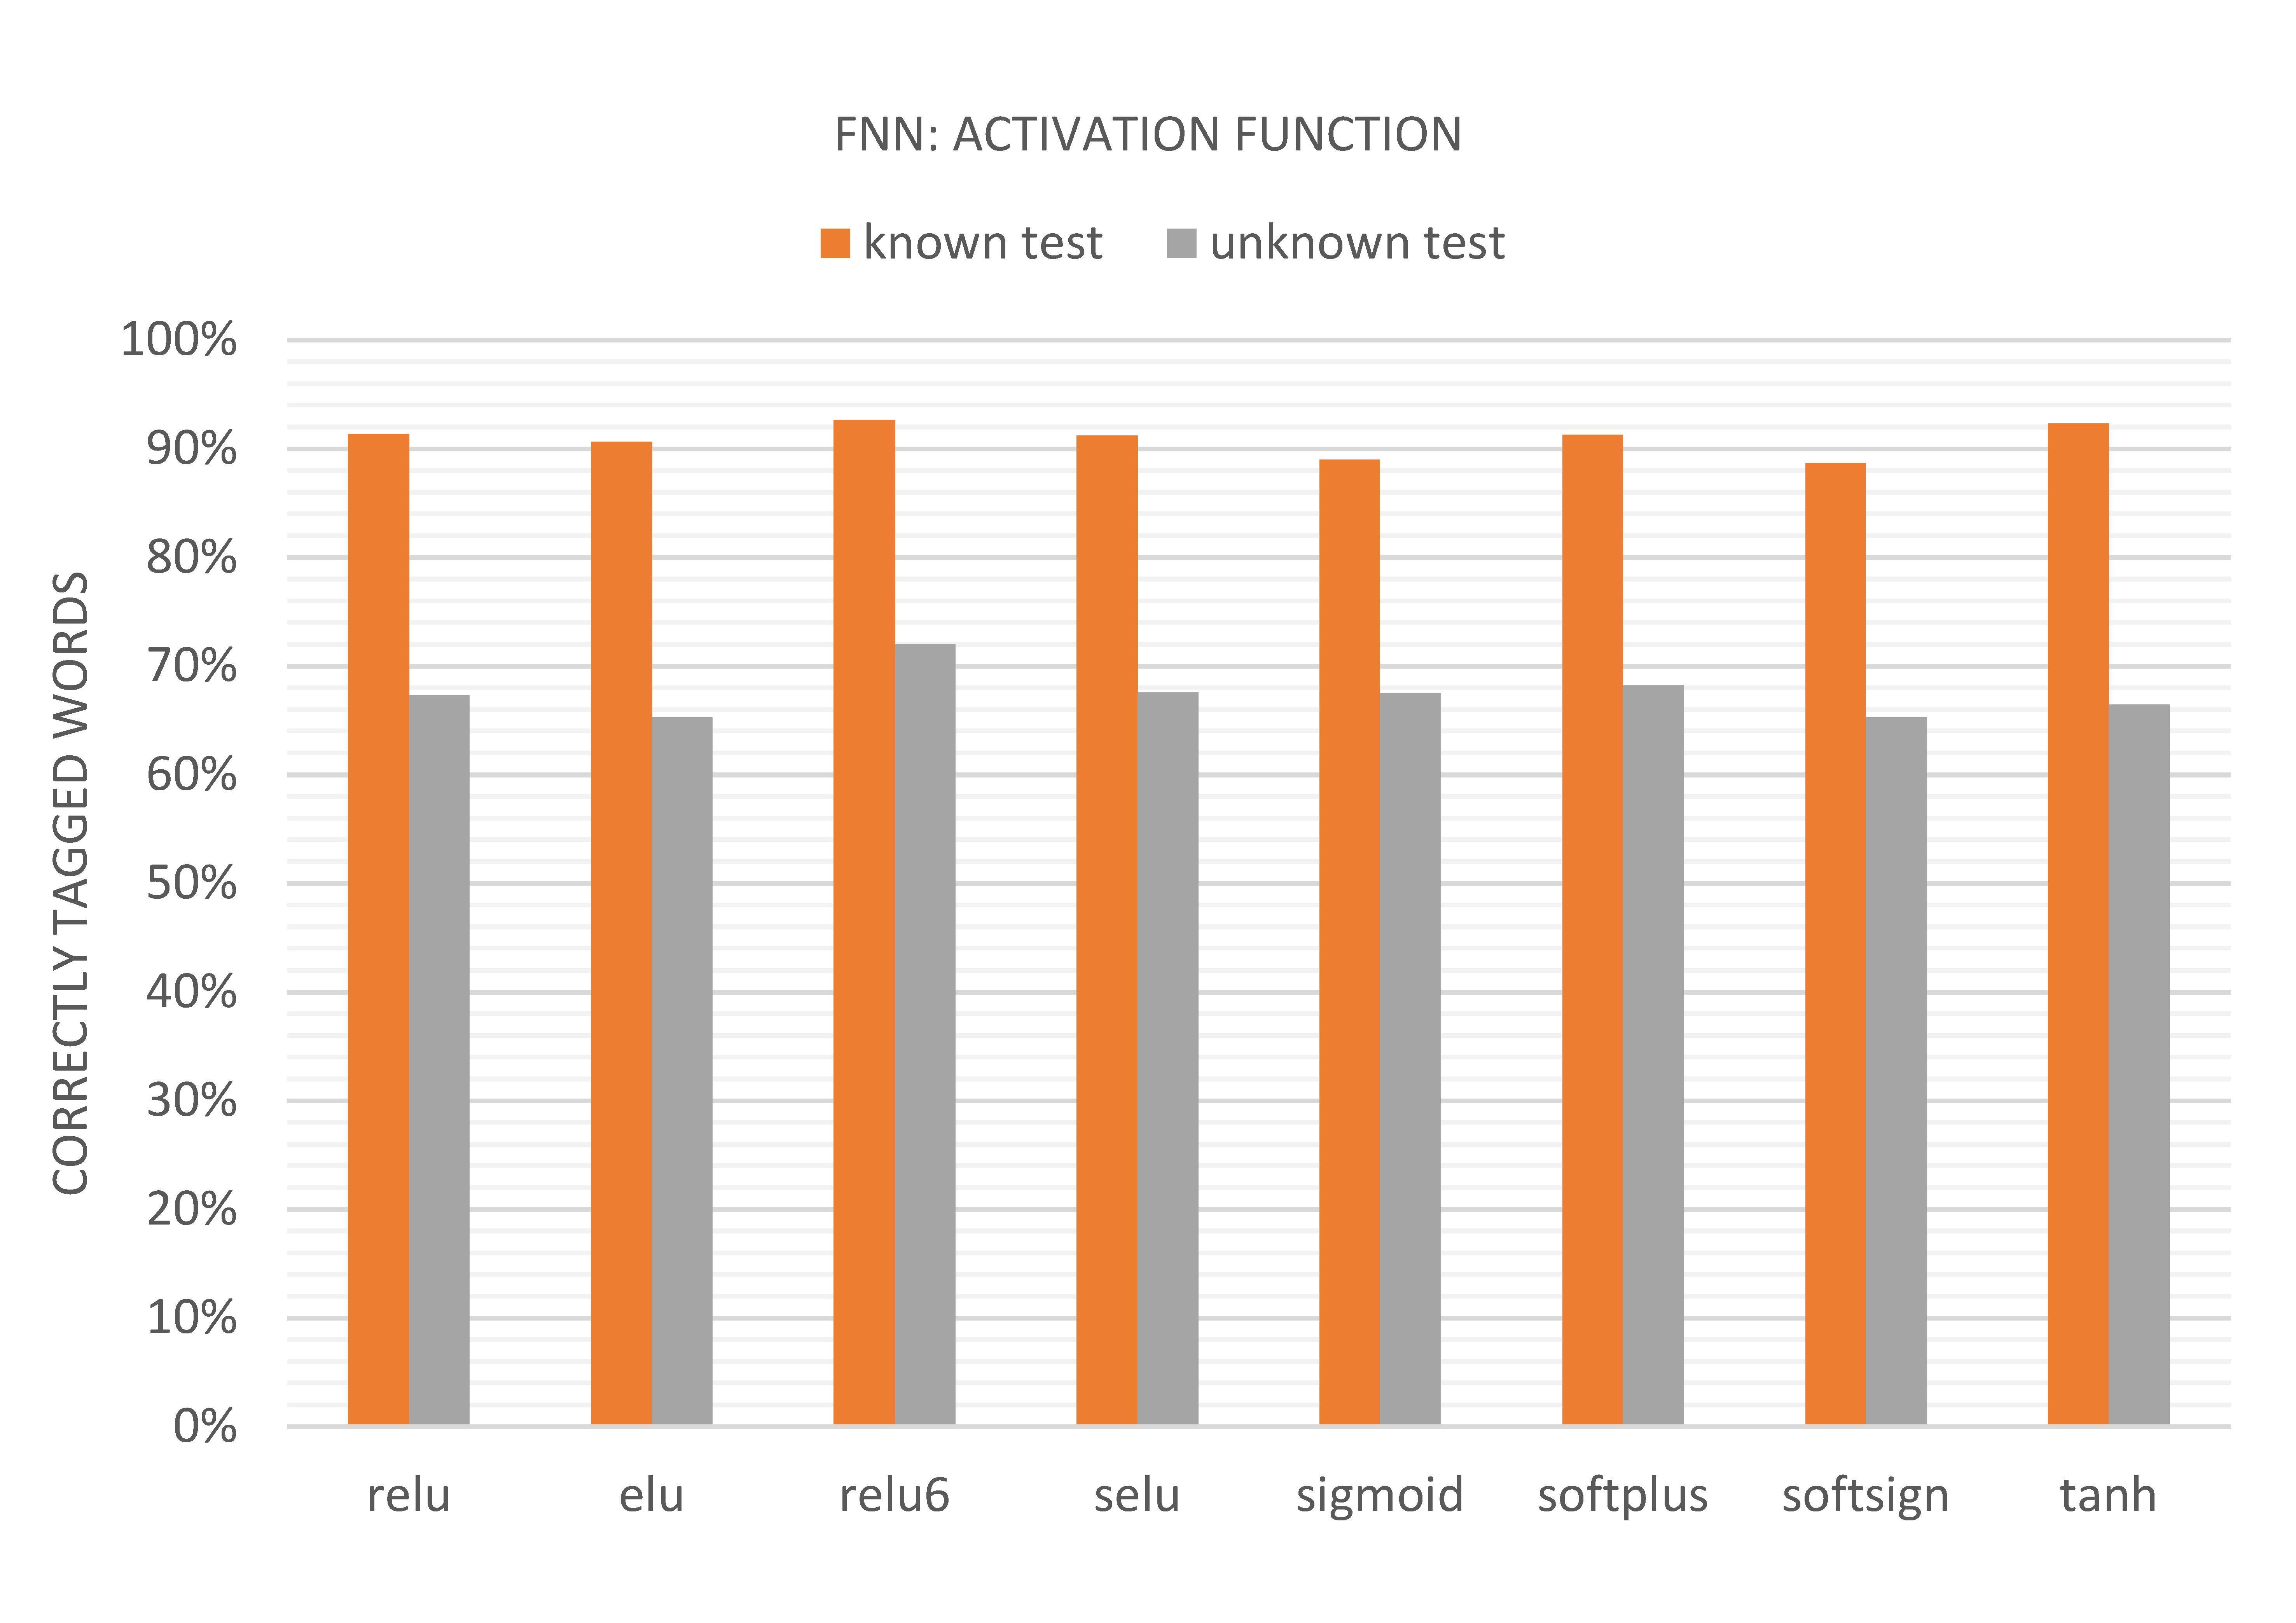
\includegraphics[width=1.07\textwidth]{images/evaluation_fnn_a}
	\caption[FNN Evaluation: Activation Function]{The evaluation results of the FNN for parameter $a$: the activation function.}
	\label{f.evaluation.fnn.a}
\end{figure}

For the known test, the model using \tt{RELU6} as activation function achieves the highest accuracy with 92.6\% correctly tagged words and the highest kappa score with $\kappa=0.818$. The same model also outperforms the other models for the unknown test, reaching an accuracy of 72.0\% and $\kappa=0.654$.

Considering the evaluation results of all 8 training groups for the FNN, the model with the following parameter configuration was found to achieve the highest accuracy, as well as the highest kappa value: one preceding word, embedding size of 250, hidden layer size of 350, 5 training epochs and \tt{RELU5} as the activation function.

\subsection{Recurrent Neural Network Models}\label{c.evaluation.results.rnn}
The first training group for the RNN, \b{training group 9}, contains models trained with 12 different time steps $t$. The evaluation result is presented in Figure \ref{f.evaluation.rnn.t}.

\begin{figure}[H]
	\hspace{-5mm}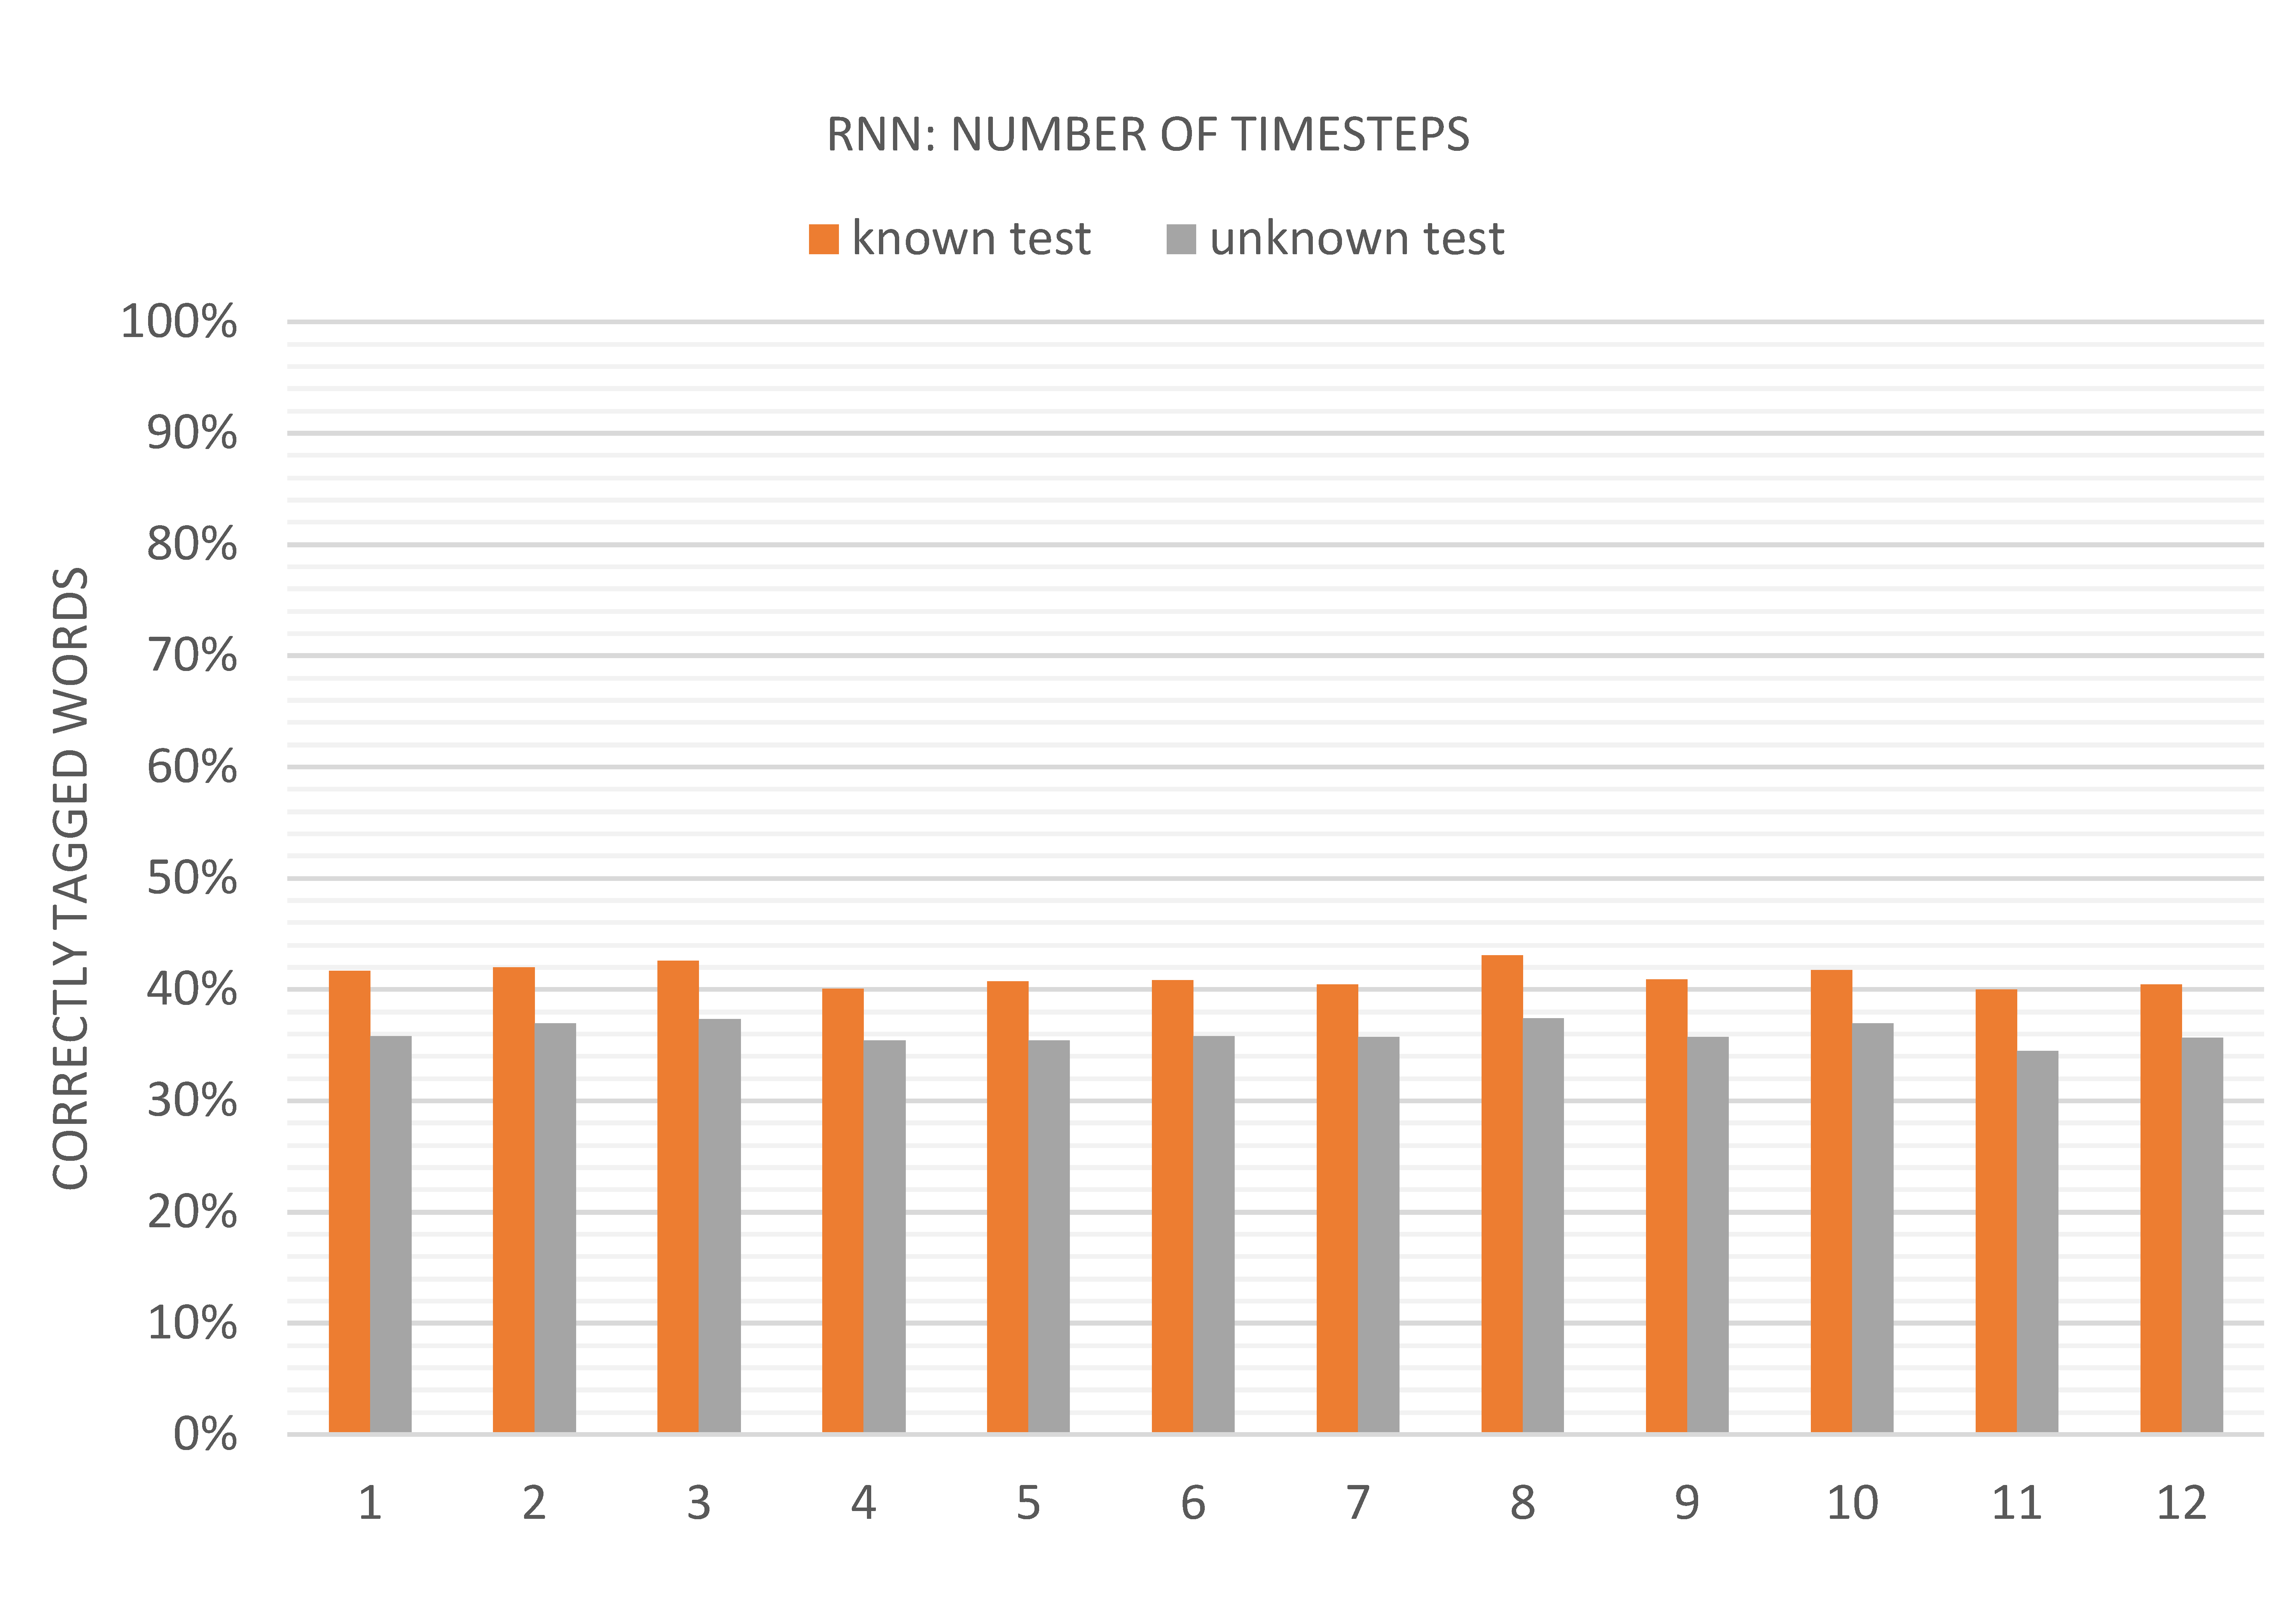
\includegraphics[width=1.07\textwidth]{images/evaluation_rnn_t}
	\caption[RNN Evaluation: Number of Time Steps]{The evaluation results of the RNN: Cohen's Kappa for parameter $t$: the number of time steps.}
	\label{f.evaluation.rnn.t}
\end{figure}

Overall, all models of the different time steps achieved similar results on both tests and there is no discernible tendency. However, for both tests, the model with $t=8$ stands out a bit with the highest accuracy of 43.1\% and $\kappa=0.341$ for the known test and 37.4\% and $\kappa=0.260$ for the unknown test.

The results of the evaluation of \b{Training group 10} that varied the size of the hidden layer $s$ is illustrated in Figure \ref{f.evaluation.rnn.s}.

\begin{figure}[H]
	\hspace{-5mm}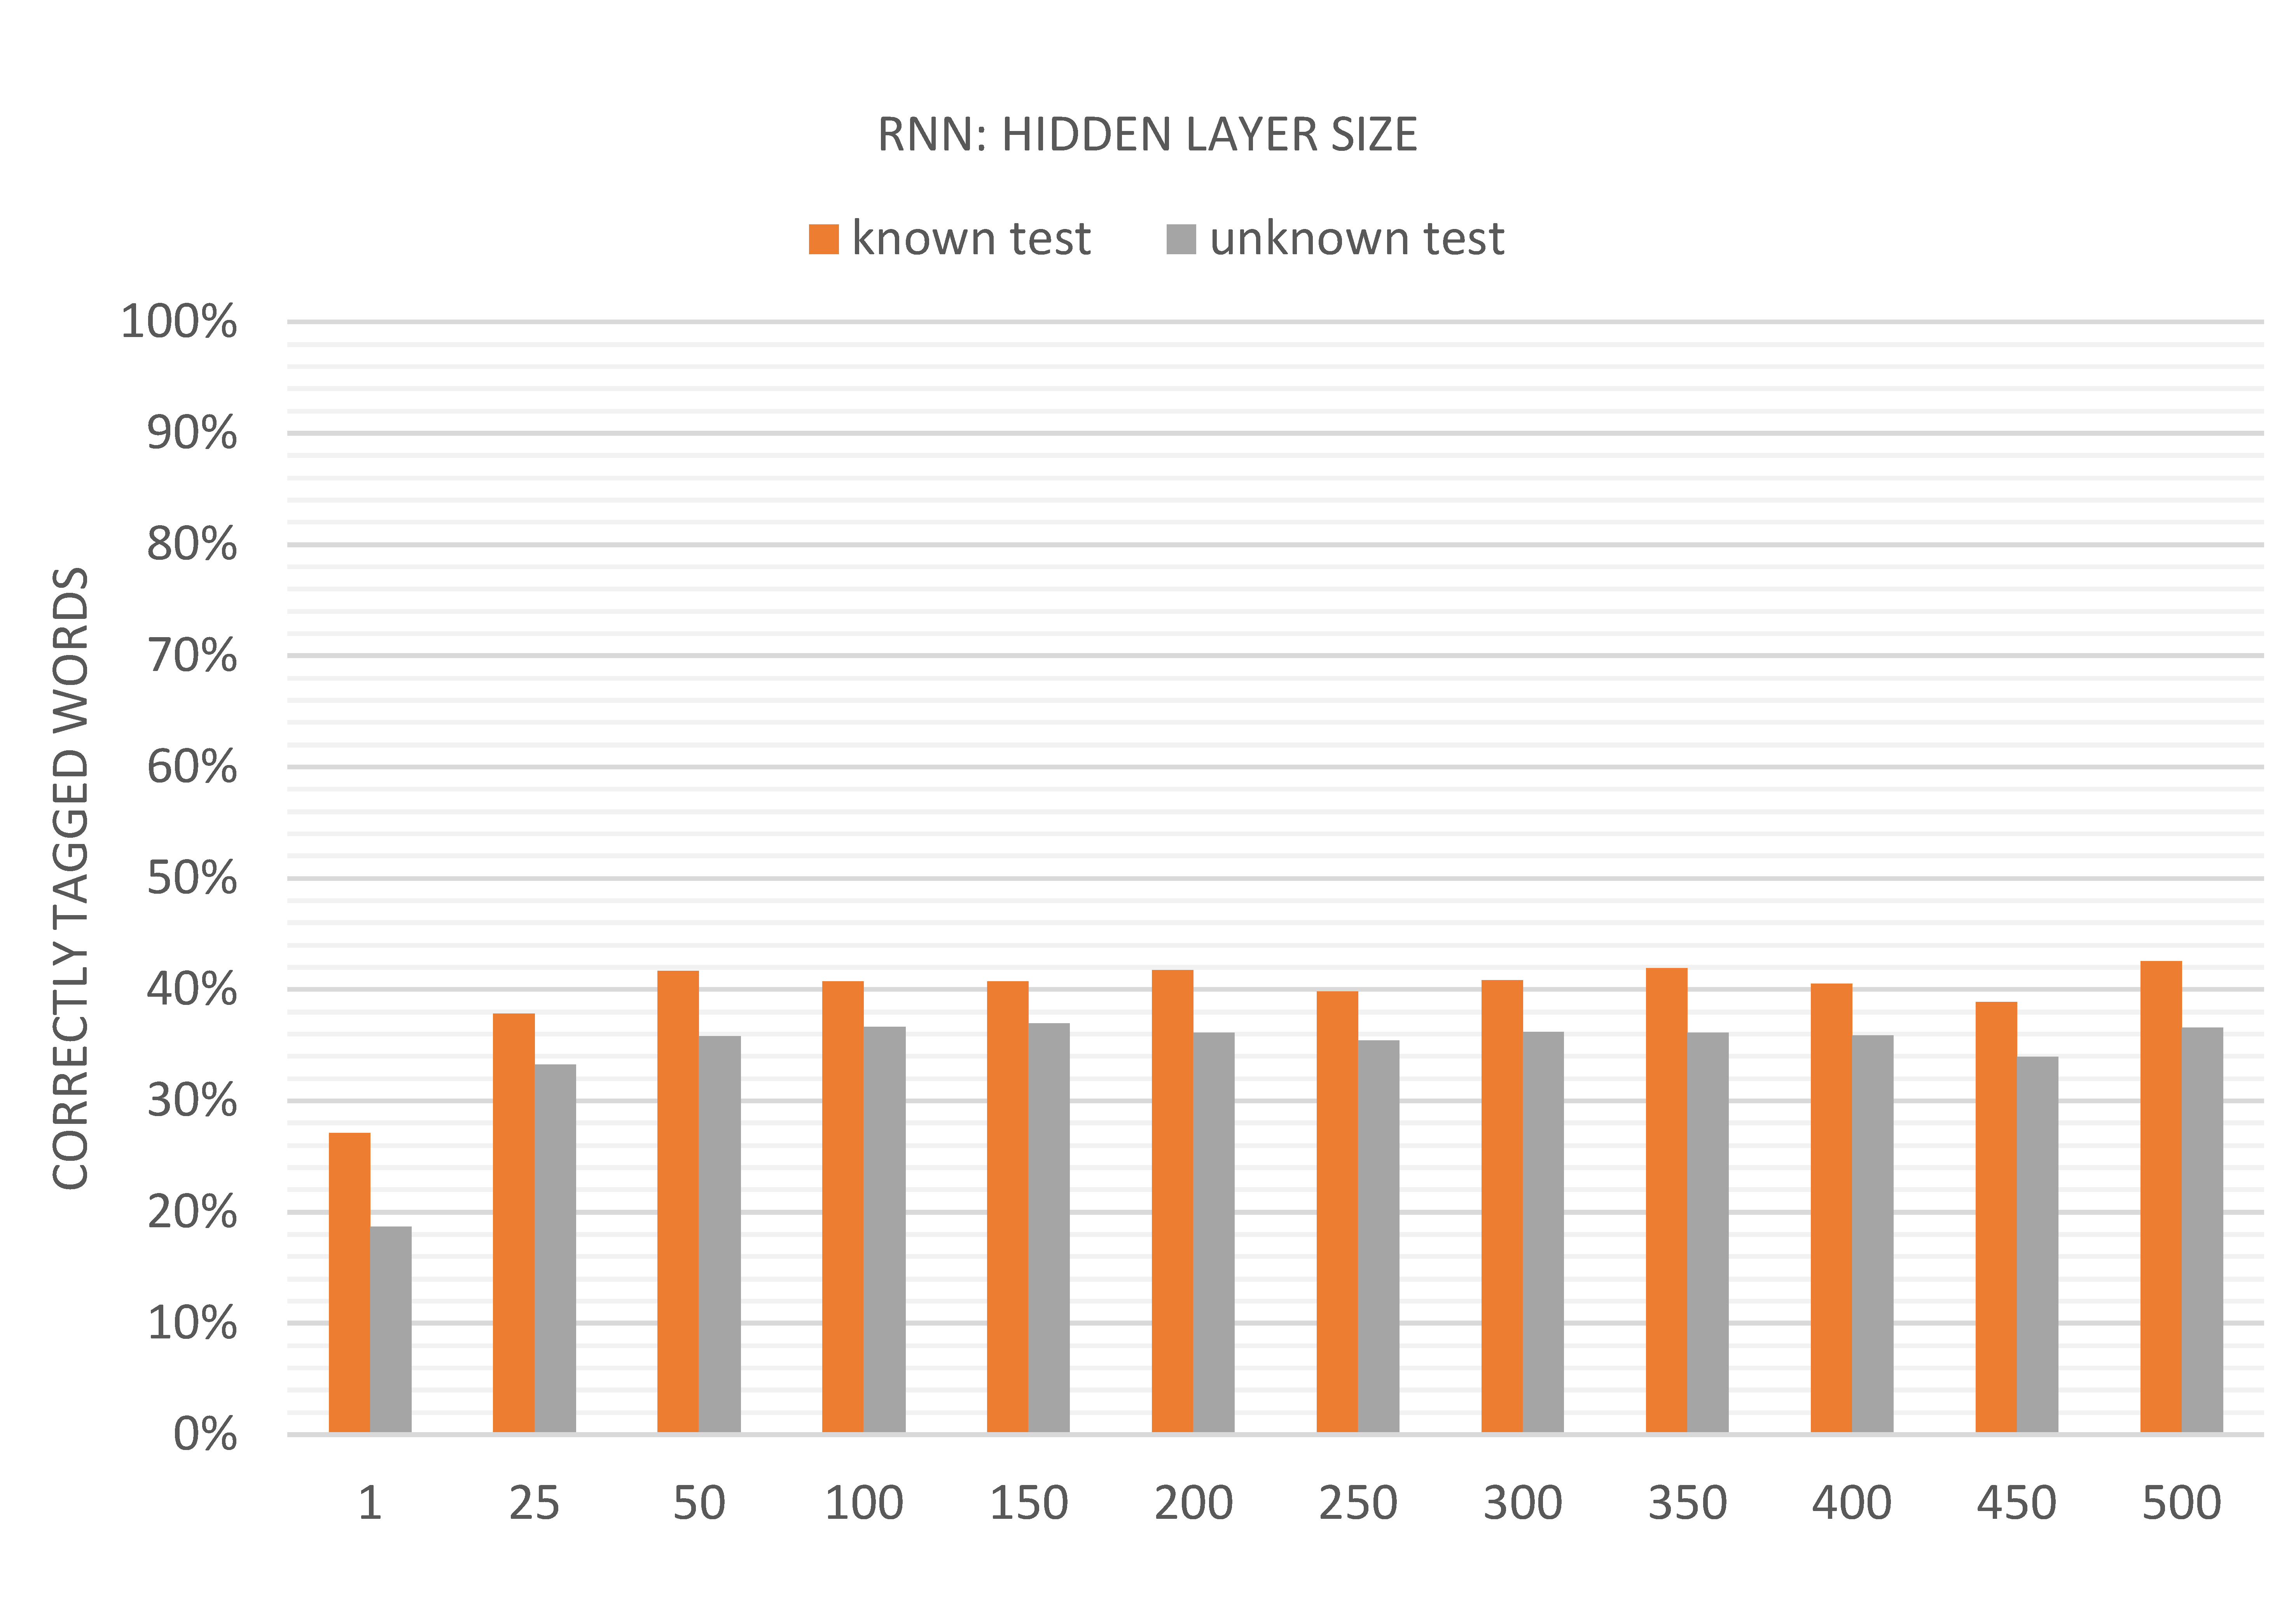
\includegraphics[width=1.07\textwidth]{images/evaluation_rnn_s}
	\caption[RNN Evaluation: Hidden Layer Size]{The evaluation results of the RNN: Cohen's Kappa for parameter $s$: the size of the hidden layer.}
	\label{f.evaluation.rnn.s}
\end{figure}

For $s\geq50$, no clear trend can be observed for both test results. Evaluating the known test, the highest accuracy of 42.6\% ($\kappa=0.333$) was reached by a model with hidden layer size $s=500$. Nevertheless, the highest kappa value $\kappa=0.334$ was assigned to the model with $s=350$, which however achieved a lower accuracy of 41.95\%. For the unknown test, the model with $s=150$ has tagged most words correctly (36.9\%, $\kappa=0.257$).

\b{Training group 11} included the evaluation with 8 different numbers of training epochs $e$. The results are presented in Figure \ref{f.evaluation.rnn.n}.

\begin{figure}[H]
	\hspace{-5mm}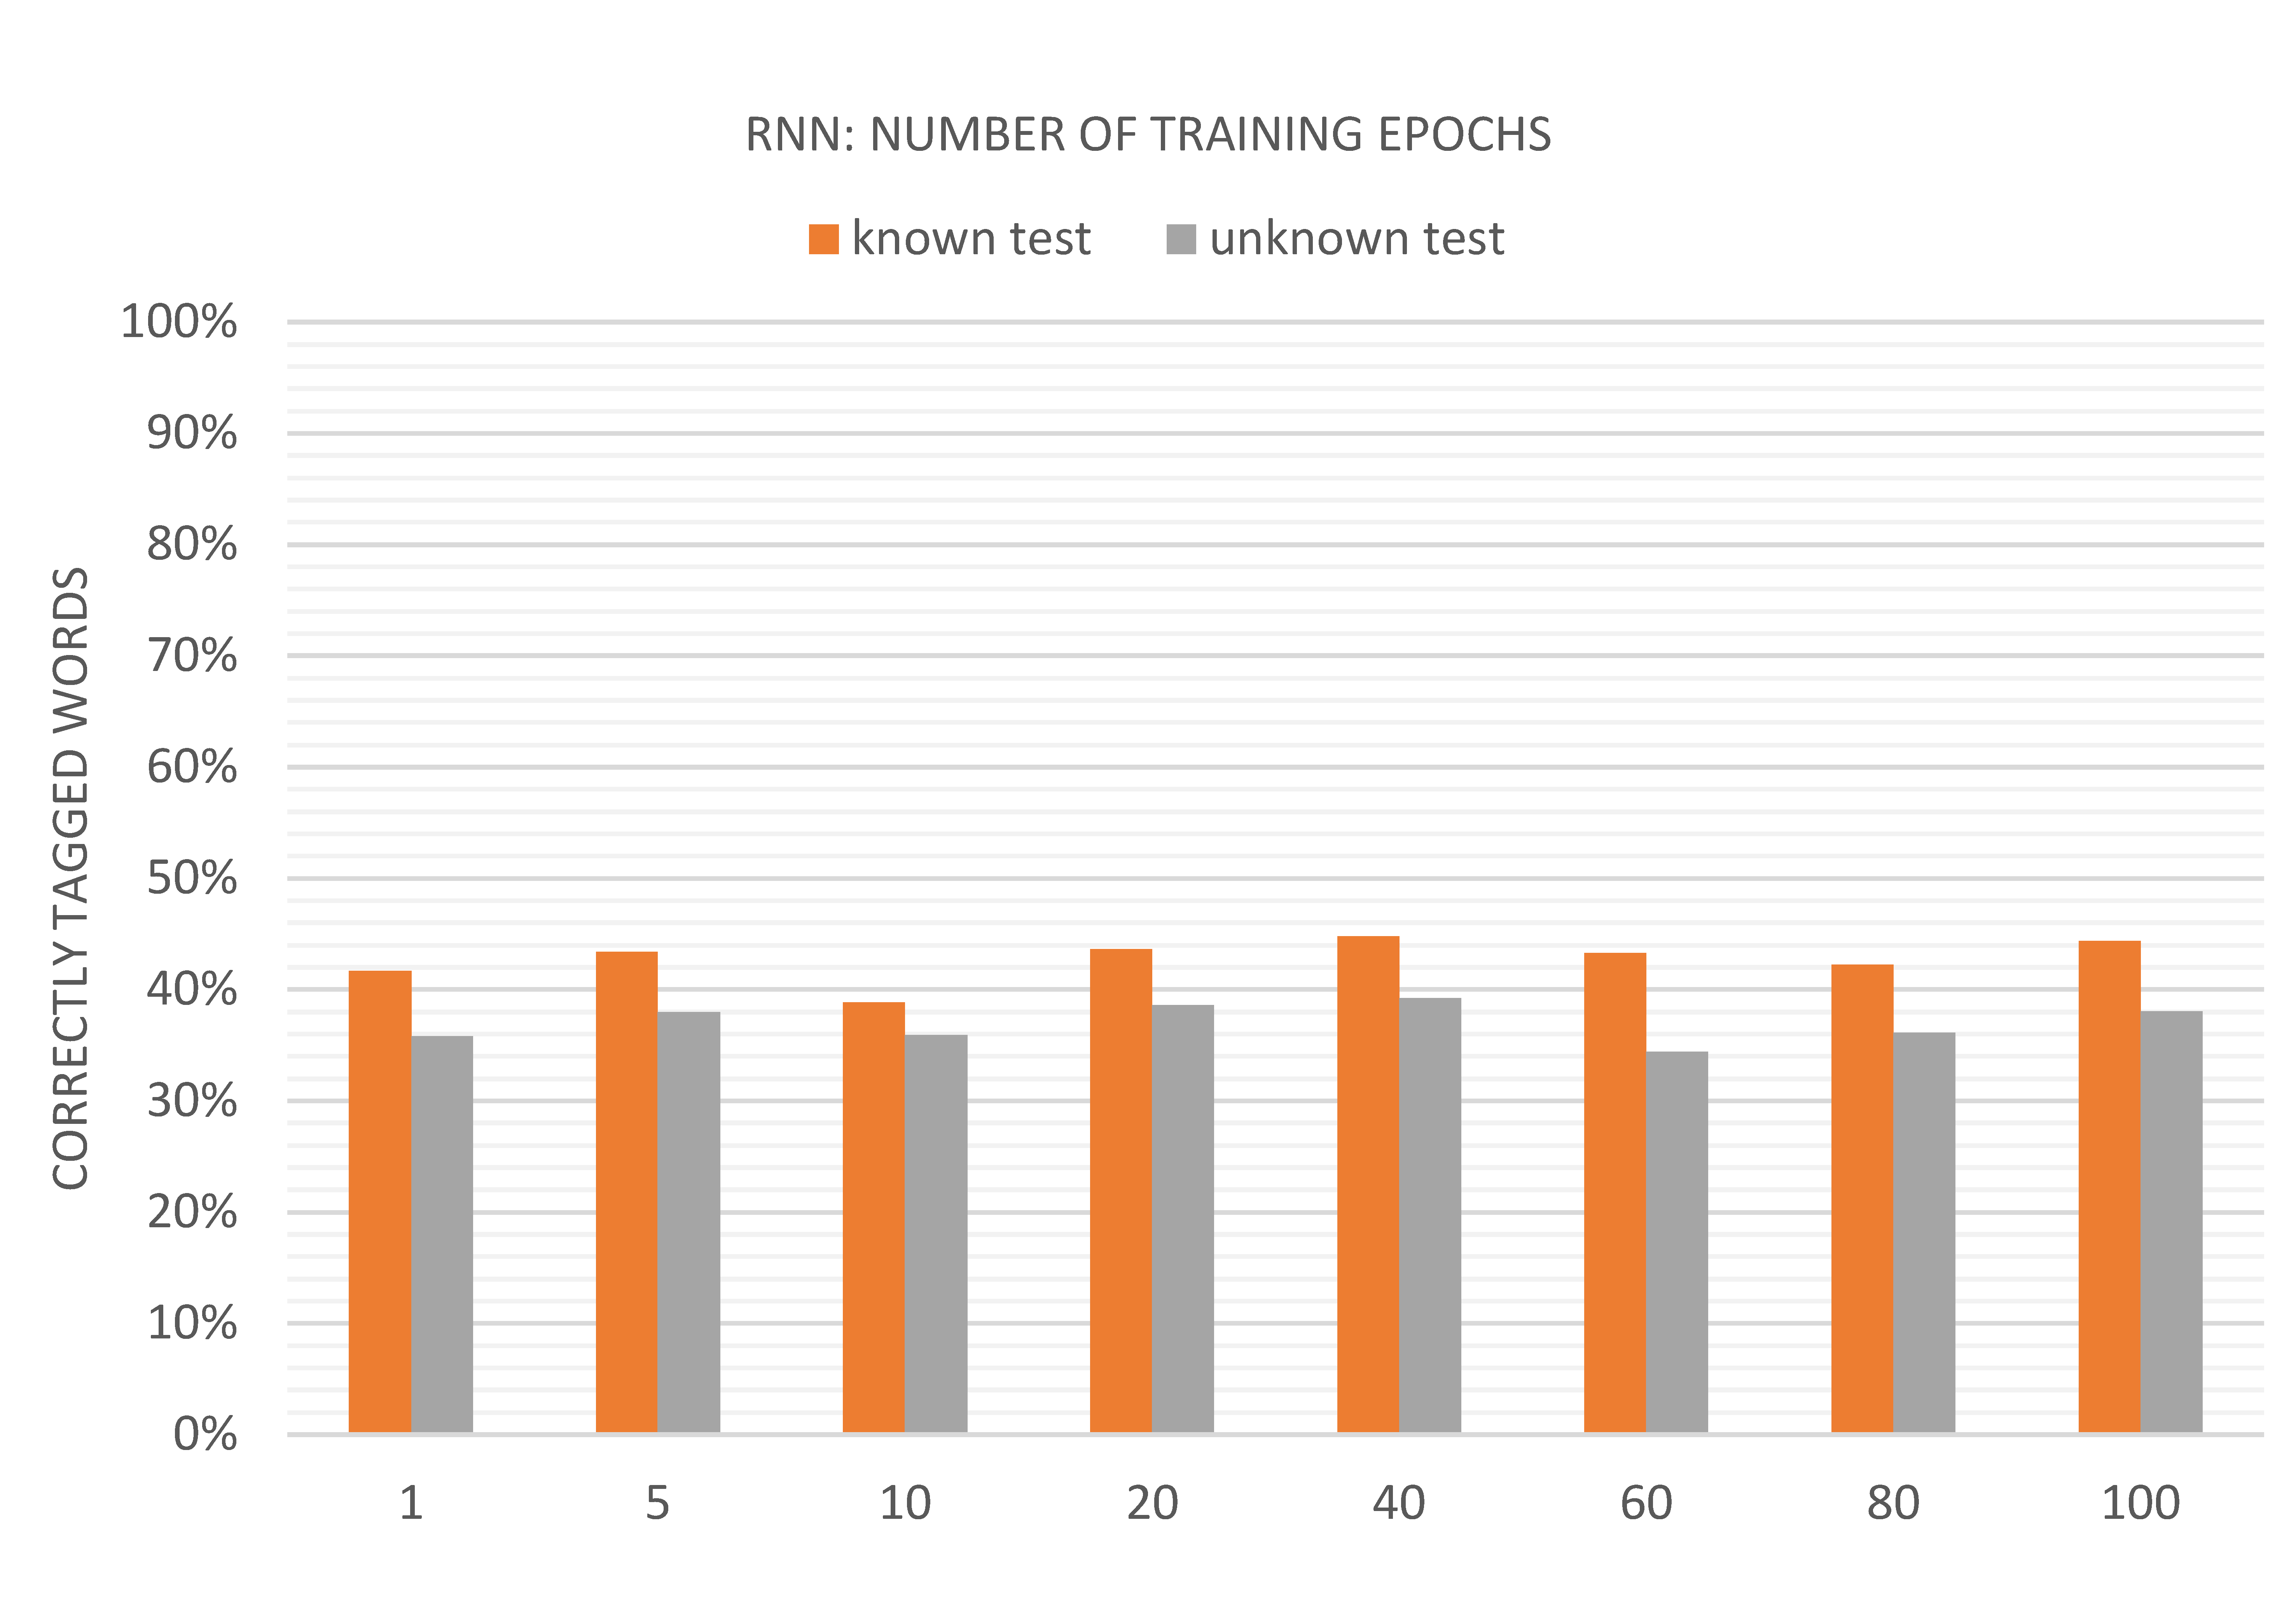
\includegraphics[width=1.07\textwidth]{images/evaluation_rnn_n}
	\caption[RNN Evaluation: Number of Training Epochs]{The evaluation results of the RNN: Cohen's Kappa for parameter $n$: the number of training epochs.}
	\label{f.evaluation.rnn.n}
\end{figure}

For the known test, the model with $n=40$ achieved the highest number of correctly tagged words of 44.8\% ($\kappa=0.356$). However, a higher kappa value $\kappa=0.359$ was reached with $n=5$. The same applies to the unknown test: $n=40$ achieved the highest accuracy 39.3\% ($\kappa=0.289$) and $n=5$ the highest kappa value $\kappa=0.291$.

The last training group, \b{training group 12}, refers to parameter $a$: the activation function (see Chapter \ref{c.postagging.fnn.architecture}). The result for the accuracy of 8 models that were trained each with another activation function is presented in Figure \ref{f.evaluation.rnn.a}. The configuration of the time step parameter was based on the results of training group 9, using $t=8$. The size of the hidden layer ($s=50$) and the number of training epochs ($n=5$) were chosen with respect to a reasonable training time.

\begin{figure}[H]
	\hspace{-5mm}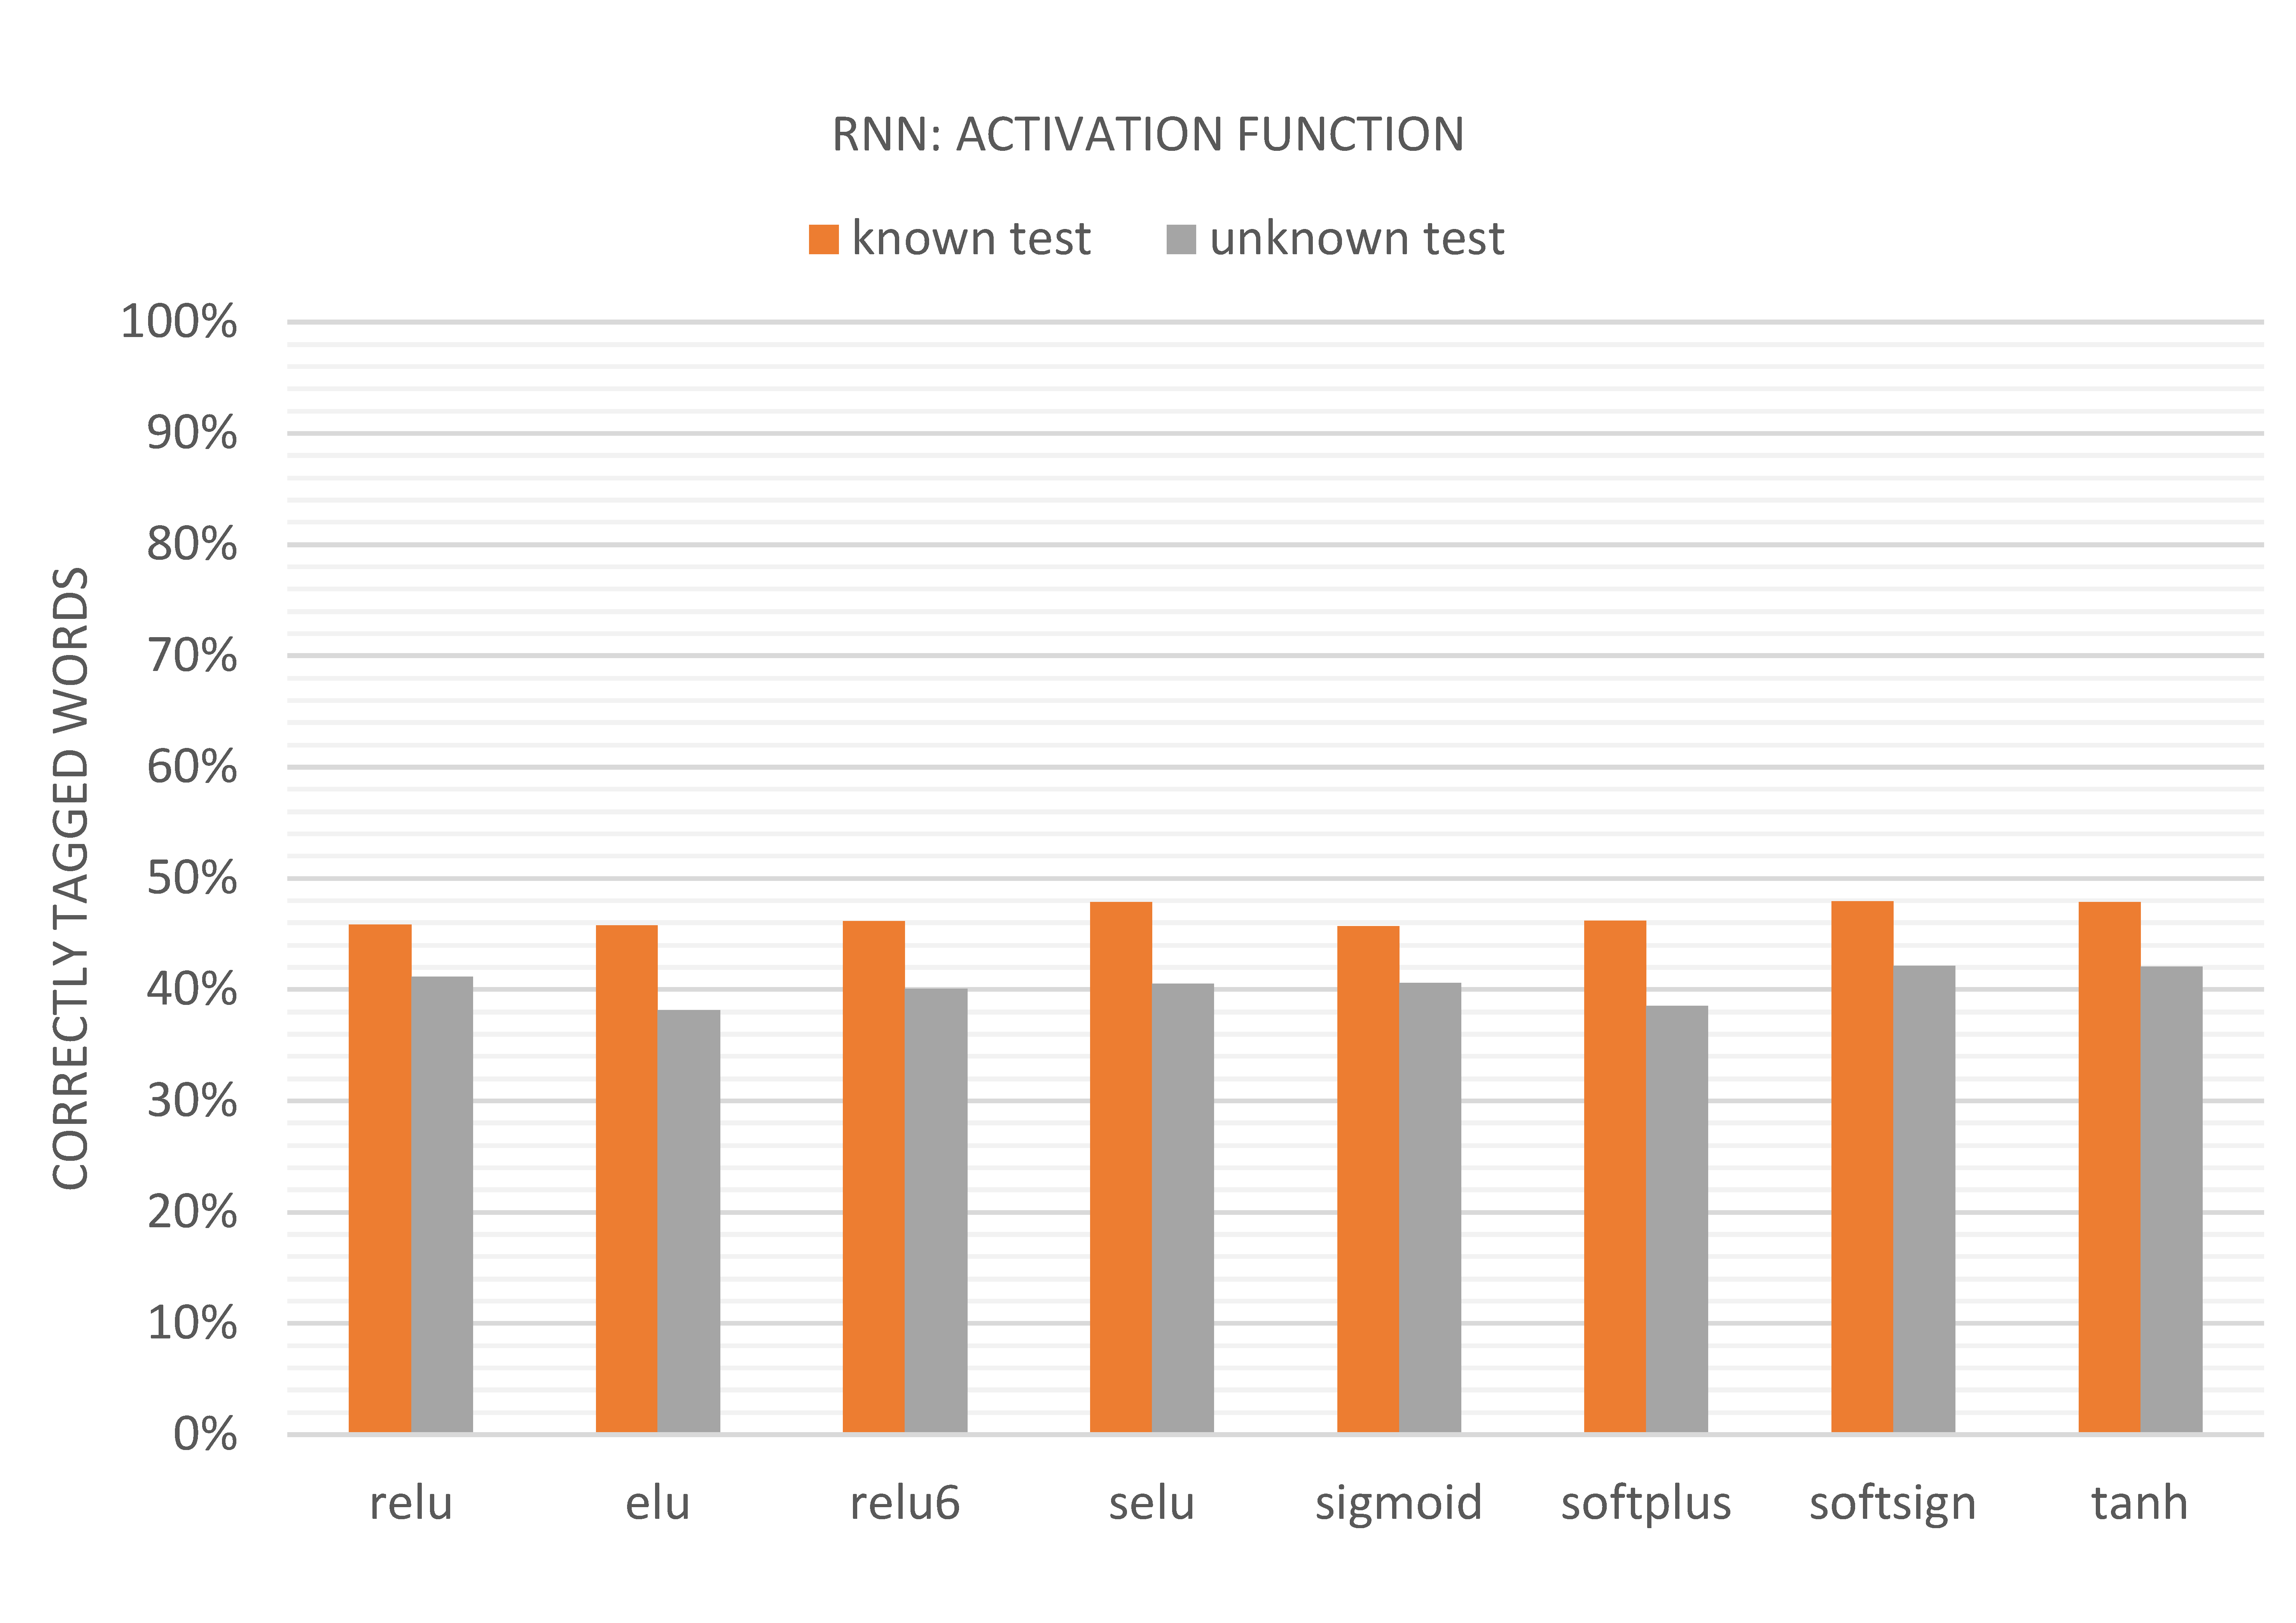
\includegraphics[width=1.07\textwidth]{images/evaluation_rnn_a}
	\caption[RNN Evaluation: Activation Function]{The evaluation results of the RNN: Cohen's Kappa for parameter $a$: the type of the activation function.}
	\label{f.evaluation.rnn.a}
\end{figure}

The best evaluation results of this training group regarding accuracy were achieved by the model utilizing the \tt{SOFTSIGN} activation function. For the known test, an accuracy of 47.95\% ($\kappa=0.403$) and for the unknown test, an accuracy of 42.1\% ($\kappa=0.324$) was achieved. However, the highest kappa values were reached by models with an activation function of \tt{SELU} ($\kappa=0.406$) and \tt{TANH} ($\kappa=0.324$).

Considering the evaluation results of all 4 training groups for the RNN, the model with the following parameter configuration was found to achieve the highest accuracy: 8 time steps, hidden layer size of 50, 5 training epochs and \tt{SOFTSIGN} as activation function.

\subsection{Hidden Markov Models}\label{c.evaluation.results.hmm}
After evaluating the neural network based language models, the HMM is evaluated in the following. For this purpose, the previous HMM (also called \i{HMM1}) which was trained on the basis of the training data generated by T. Michael \cite{michael2016} is compared to a new HMM (\i{HMM2}) trained on the basis of the training data proposed in this thesis. The evaluation was carried out using the known and the unknown test developed in this thesis; the results are presented in Figure \ref{f.evaluation.hmm}.

\begin{figure}[H]
\centering
\subcaptionbox{HMM\label{f.evaluation.hmm.a}}
{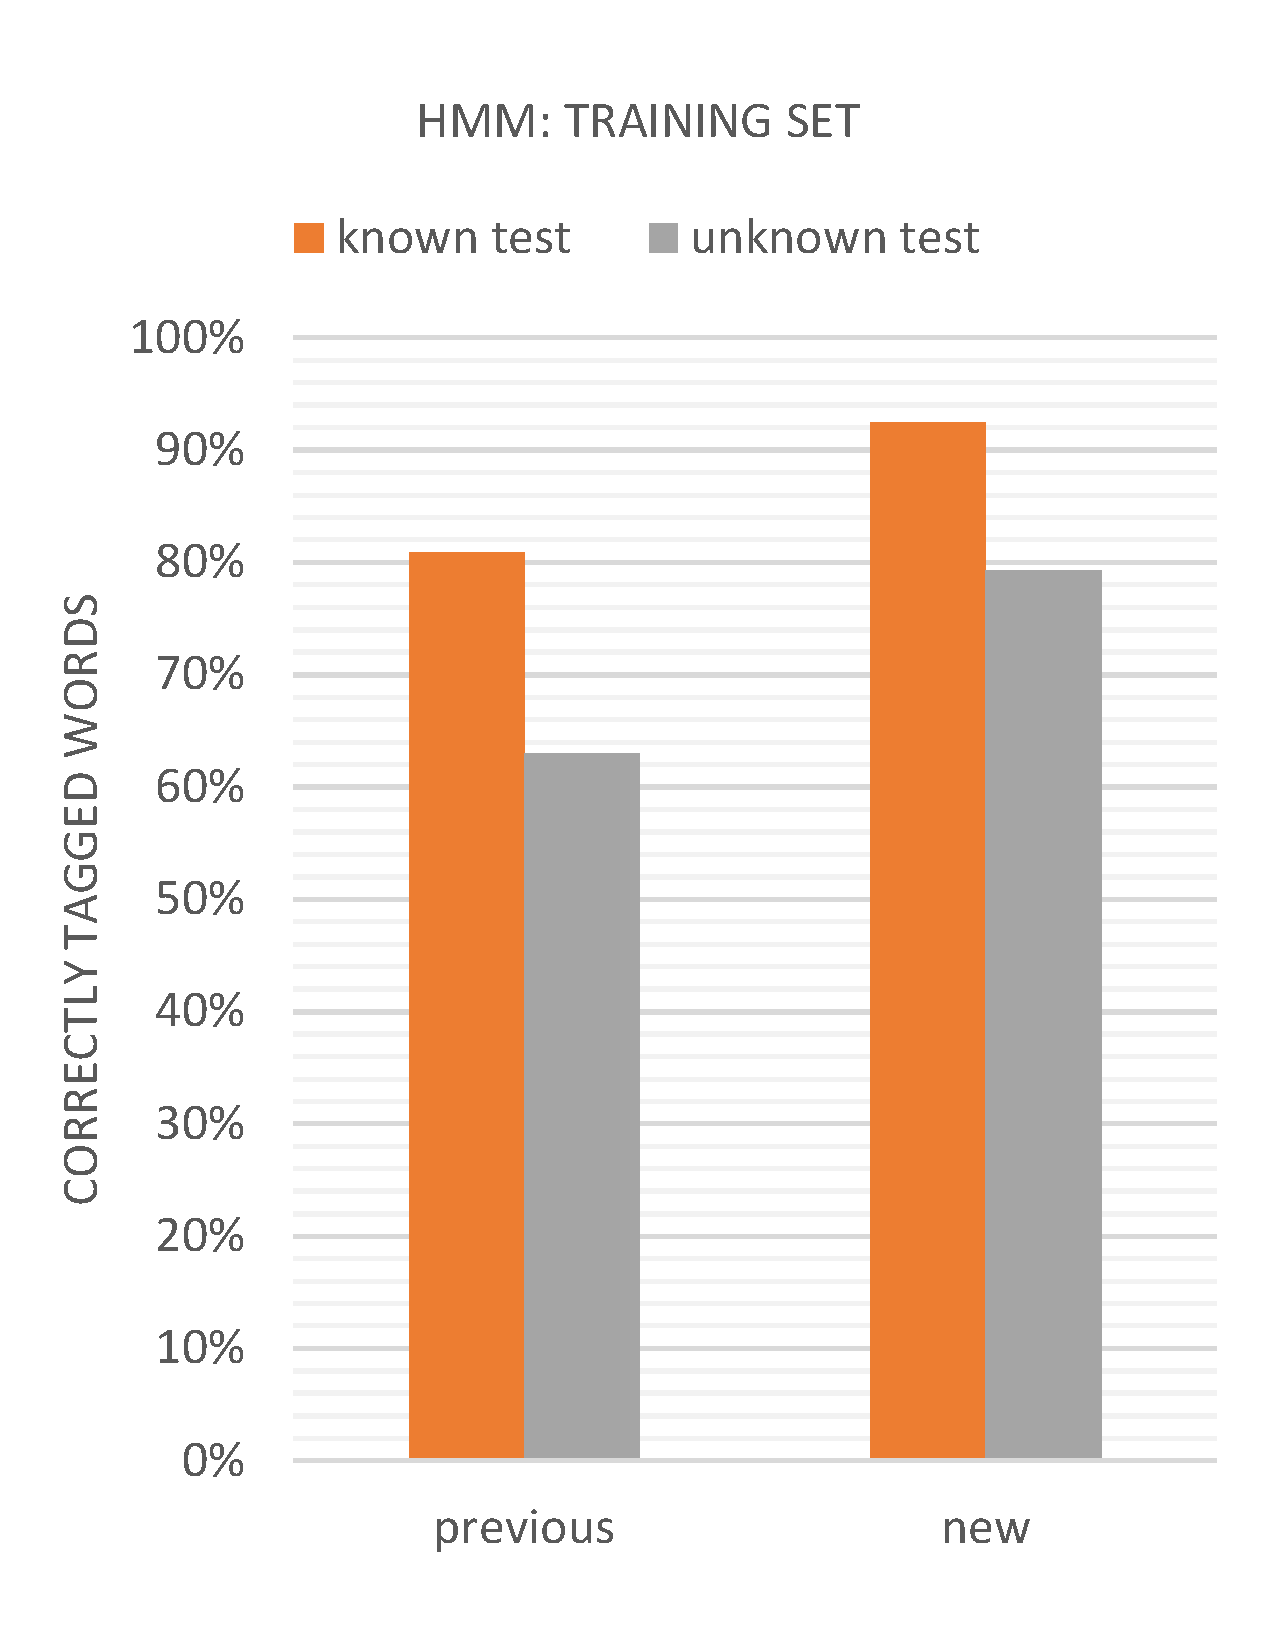
\includegraphics[width=0.495\textwidth]{images/evaluation_hmm}}
\subcaptionbox{HMM with Kappa\label{f.evaluation.hmm.k}}
{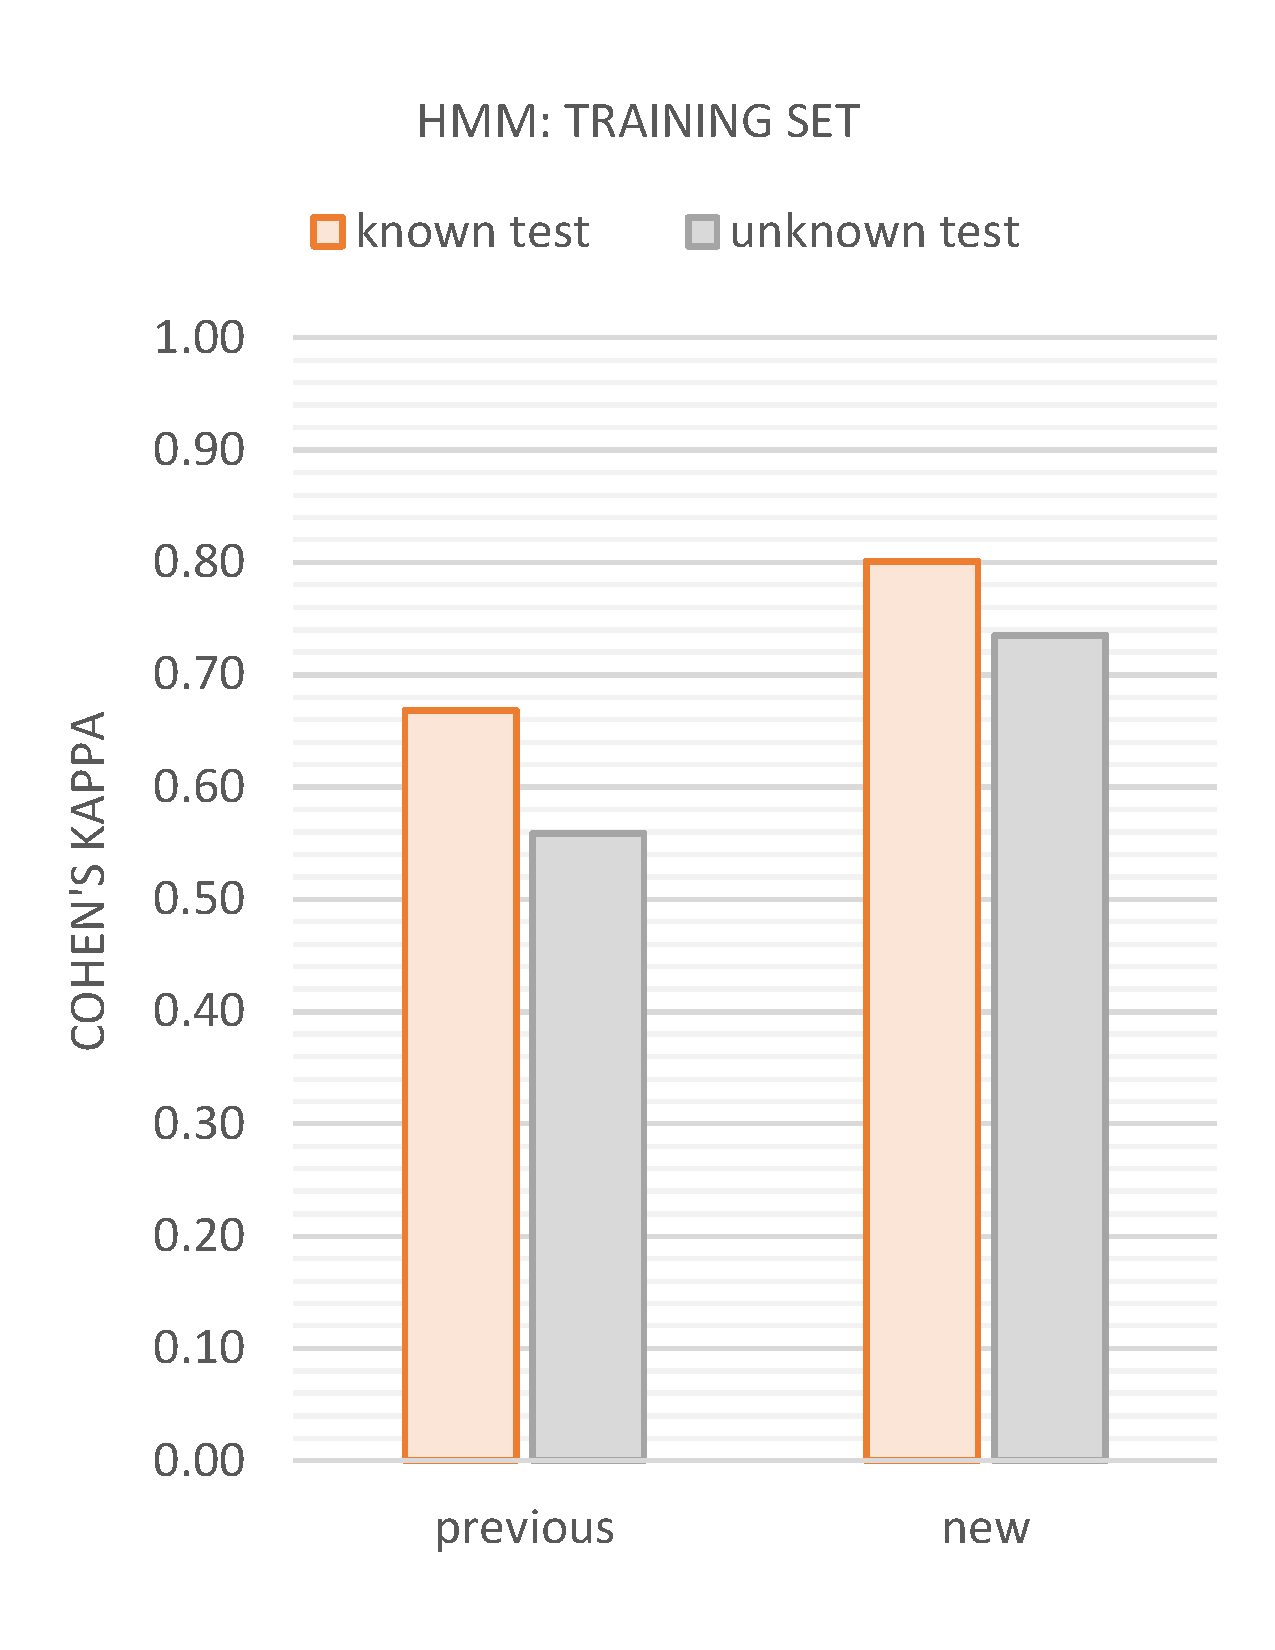
\includegraphics[width=0.495\textwidth]{images/evaluation_hmm_k}}
\vspace{1em}
\caption[HMM Evaluation]{The evaluation results of the previous HMM trained by T. Michael \cite{michael2016} and the new HMM based on the new training data proposed in this thesis.}
\label{f.evaluation.hmm}
\end{figure}

The previous HMM tagged 82.5\% of the words of the known test and 63.0\% of the unknown test correctly, whereas it was 93.4\% for the known and 79.3\% for the unknown test for the new HMM. It was evident that the HMM, which was based on the new training data, performed significantly better than the previous HMM. Especially the result for the unknown test is remarkable, as the accuracy increases by more than 16\%.

It should be noted that the comparison of the previous and the new HMM model based on the known test has some limitations, as the known test was not fully known\footnote{As described in Chapter \ref{c.evaluation.test}, the known test contains 620 sentences. 388 sentences are included in he corpus of the previous HMM, resulting in 37.4\% of the sentences of the known test, that were unknown to the previous HMM.} to the previous HMM. Nevertheless, the major part of the known test set was based on training templates that were already used to build the corpus for the previous HMM, which is why it still scored well with more than 4 correct tags out of 5.

\section{Overall Comparison}\label{c.evaluation.comparison}
After evaluating the neural network models and the hidden Markov models separately, the different architectures will now be compared to each other. For this purpose, the evaluation results of the best FNN model proposed in Chapter \ref{c.evaluation.results.fnn}, the best RNN model found in Chapter \ref{c.evaluation.results.rnn} and the two HMM models evaluated in Chapter \ref{c.evaluation.results.hmm} are summarized in Table \ref{t.evaluation.comparison} and illustrated in Figure \ref{f.evaluation.comparison}.

\vspace{.5em}
\begin{table}[!ht]
	\centering
	\hfill
	\subcaptionbox{Known Test\label{t.evaluation.comparison.known}}
	{\centering\small\def\arraystretch{1.5}\begin{tabular}{ c c c }
	\trule
	 & \textsc{Accuracy} & \textsc{Kappa} \\
	\srule
	HMM1 & 80.87\%     & 0.668     \\
	\mrule
	HMM2 & 92.43\%     & 0.801     \\
	\mrule
	FNN  & \b{92.63\%} & \b{0.818} \\
	\mrule
	RNN  & 47.95\%     & 0.403     \\
	\brule
	\end{tabular}}
	\hfill
	\subcaptionbox{Unknown Test\label{t.evaluation.comparison.unknown}}
	{\centering\small\def\arraystretch{1.5}\begin{tabular}{ c c c }
	\trule
	 & \textsc{Accuracy} & \textsc{Kappa} \\
	\srule
	HMM1 & 62.99\%     & 0.559     \\
	\mrule
	HMM2 & \b{79.29\%} & \b{0.735} \\
	\mrule
	FNN  & 72.01\%     & 0.654     \\
	\mrule
	RNN  & 42.11\%     & 0.321     \\
	\brule
	\end{tabular}}
	\hfill
	\vspace{.8em}
	\caption[Comparison of all Architectures]{A tabular overview of the evaluation results of HMM1 trained by T. Michael \cite{michael2016}, HMM2 trained on the new training data proposed in this thesis and the FNN and RNN model with the highest accuracy according to the evaluation of the different training groups.}
	\label{t.evaluation.comparison}
\end{table}

\begin{figure}[H]
\centering
\subcaptionbox{Comparison of the accuracy\label{f.evaluation.comparison.a}}
{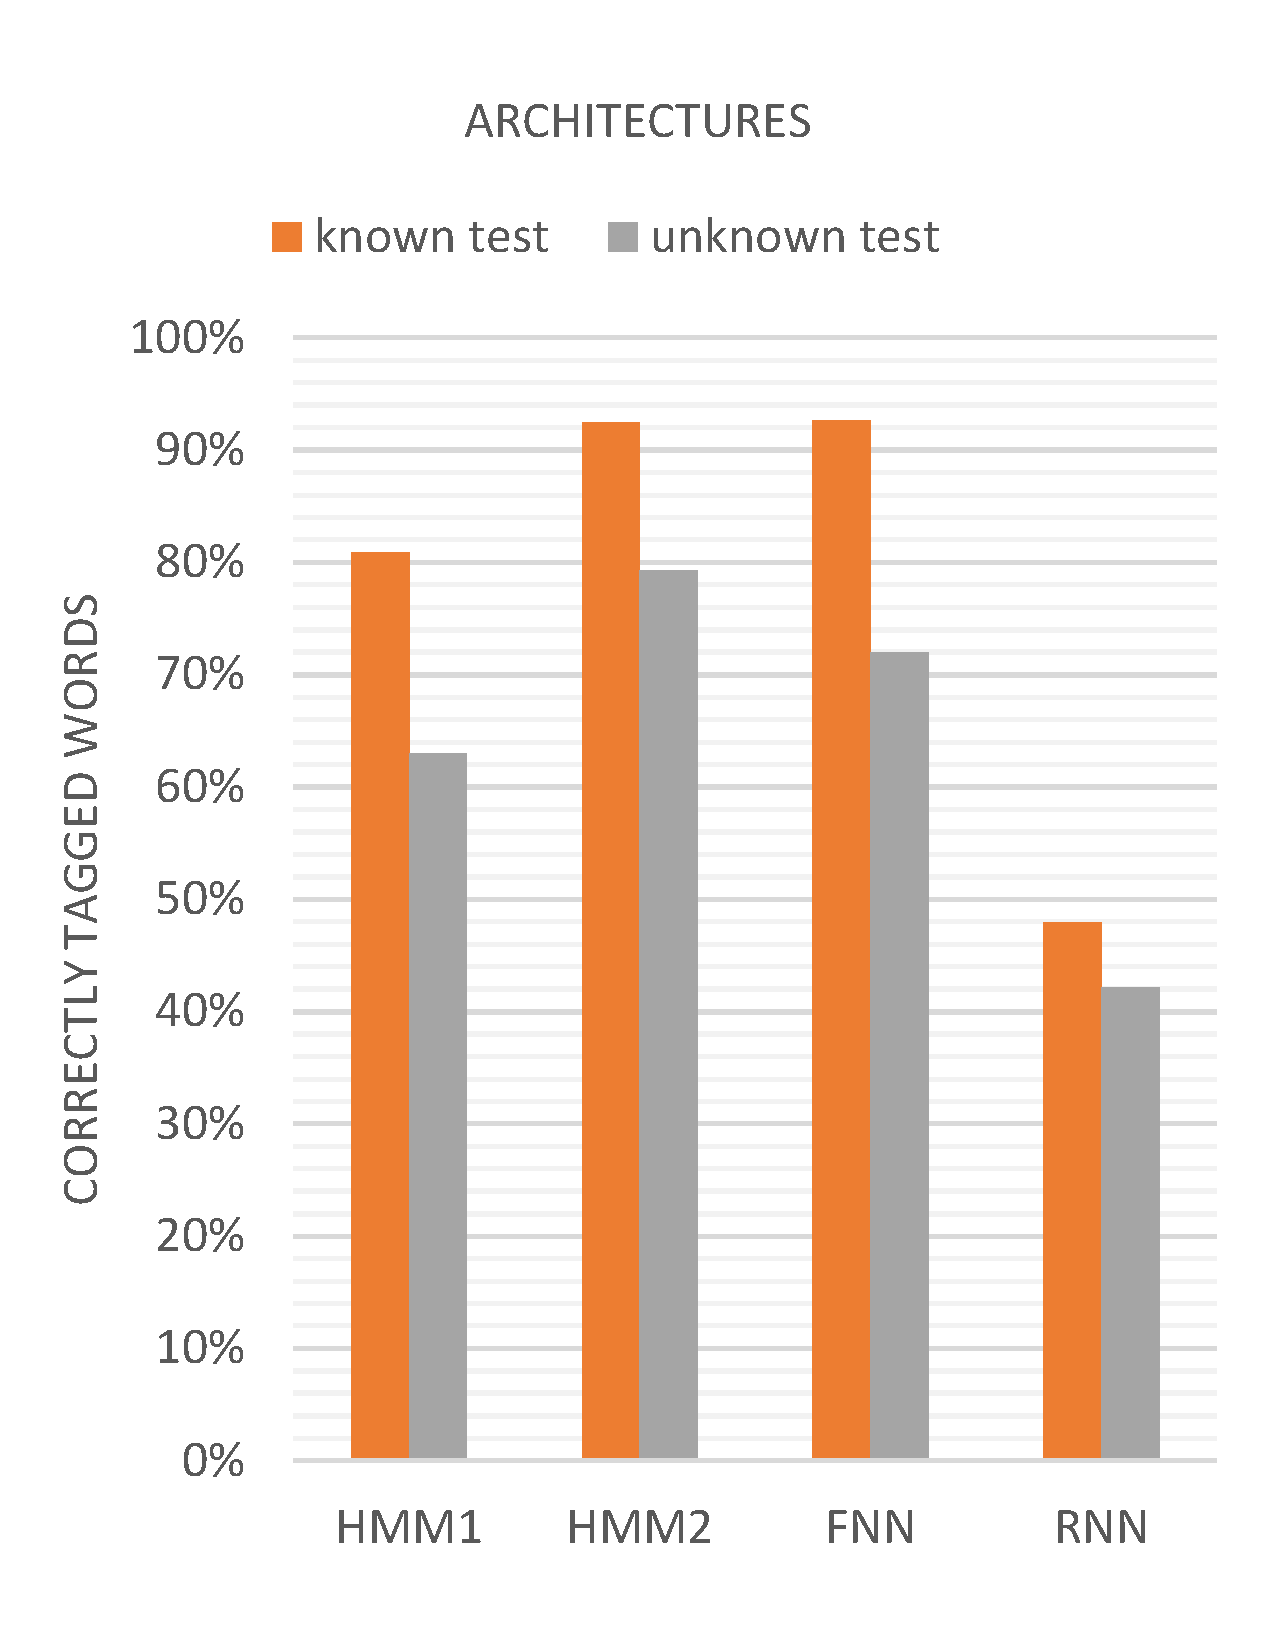
\includegraphics[width=0.495\textwidth]{images/comparison}}
\subcaptionbox{Comparison of the kappa score\label{f.evaluation.comparison.k}}
{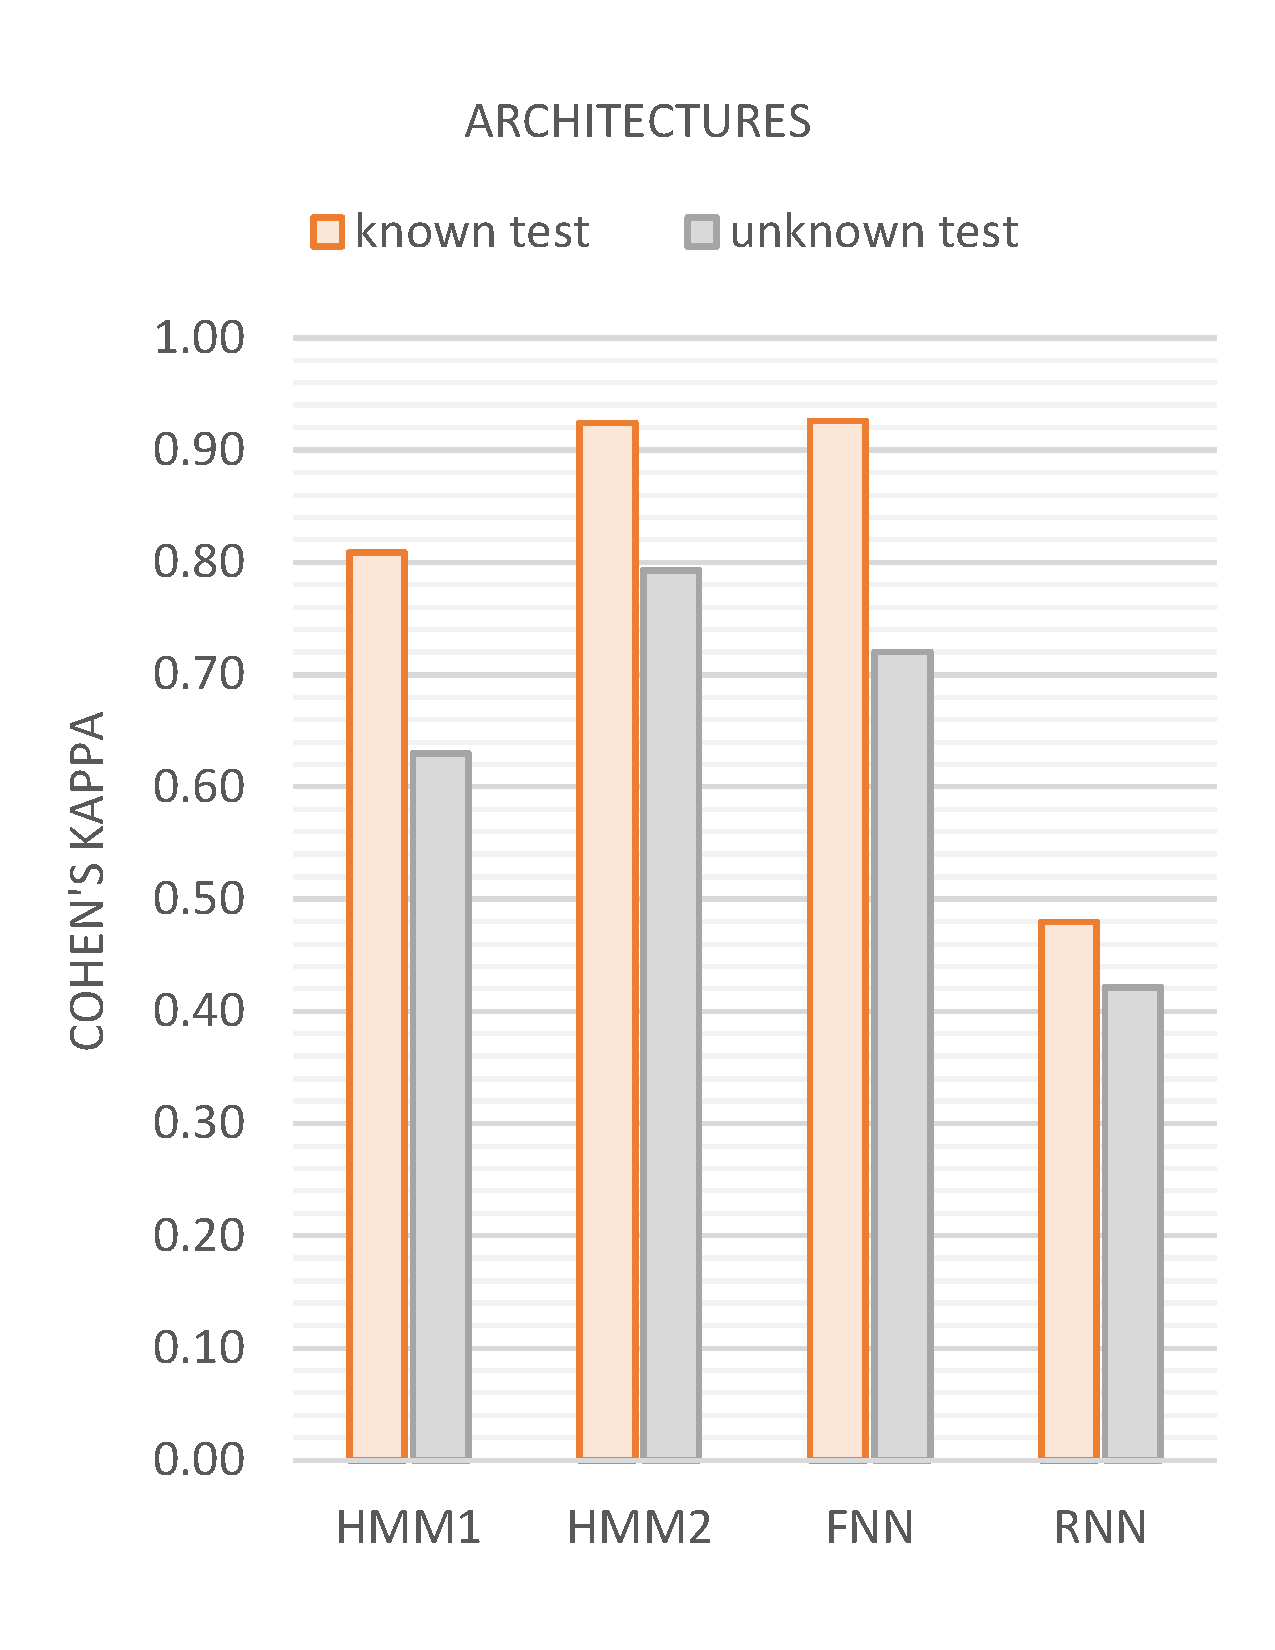
\includegraphics[width=0.495\textwidth]{images/comparison_k}}
\vspace{1em}
\caption[Comparison of all Architectures]{The evaluation results of the previous HMM model trained by T. Michael \cite{michael2016}, the new HMM model trained on the new training data proposed in this thesis, the best FNN and the best RNN model according to the evaluation of the different training groups.}
\label{f.evaluation.comparison}
\end{figure}

The FNN model achieved the highest accuracy as well as the highest kappa score for the known test, closely followed by the HMM2 model, which was only slightly less accurate. The difference between these two models is only 0.2\% ($\Delta\kappa=0.017$). With a kappa score of more than 0.8, both models offer a very good agreement with the labeled test data. However, the HMM1 model still reached a good agreement. The RNN model tagged less than 50\% of the words of the known test correctly, thus barely reaching a moderate agreement with the labeled test data.

The result of the unknown test is a bit more distinctive. The highest accuracy as well as the highest kappa score was reached by the HMM2 model, followed by the FNN model with a difference of 7.28\% ($\Delta\kappa=0.084$). With a kappa score of more than 0.6, both models offer a good agreement with the labeled test data, whereas the FNN1 model reaches a moderate agreement. Similarly to the known test result, the RNN tagged less than 50\% of the words correctly, offering only a fair agreement with the labeled test data.

Overall, every model achieved a higher accuracy and a higher kappa score on the know test than on the unknown test. While this is an expected result, the differences between the accuracy of known and unknown test vary for each model. While this difference is relatively small for the RNN model (5.84\%), the models of HMM1 and HMM2 show differences of 17.88\% and 13.14\%. The largest difference can be observed in the FNN model, which tagged an additional 20.63\% of the words of the known test correctly, compared to those of the unknown test.

% ===================================================================================
\chapter{Discussion and Conclusion}\label{c.conclusion}
The final chapter summarizes the work of this thesis and the evaluation results achieved. It discusses the evaluation findings and reveals potential areas for further research based on the knowledge gained in this thesis.

\section{Summary}\label{c.conclusion.summary}
The aim to develop a neural network based part-of-speech tagger for the advisory Artificial Conversational Agent \Alex\ was accomplished within the scope of this thesis.

The different modules of \Alex\ were analyzed to gain information about its language processing, the generation of training data and the hidden Markov model tagger and its interface.

Based on this knowledge, a tagger module was implemented featuring a feed-forward neural network as well as a recurrent neural network architecture. A training corpus containing tagged sentences was generated with the help of an improved set of sentence templates. With both neural network architectures, several language models were trained on this corpus using parameter variation. These models were then evaluated with two corresponding tests sets, containing sentences from the training corpus (known data) and unknown sentences, that were derived from user log data. Furthermore, both the hidden Markov model, which \Alex\ already utilizes for POS tagging and an HMM that was trained on the new training data, proposed in this thesis, were evaluated with these test sets.

After evaluating the trained language models, it could be shown that the HMM based on new training data significantly performed better than the previous HMM tagger, especially on unknown data. It was also shown that a tagger based on a feed-forward neural network was able to outperform this new HMM tagger on known evaluation data.

\section{Discussion}\label{c.conclusion.discussion}
According to the evaluation results, the FNN model achieved the highest accuracy for known data and would therefore be preferred for productive use. However, the HMM model performed significantly better on unknown data. Given the fact that a chatbot has to deal with a lot of unknown input data due to users that do not know the limits of the chatbots knowledge and capabilities, the result of the unknown test is more important for the choice of the language model to use in \Alex.

When reviewing the overall comparison of the trained language models, it is apparent that the results of the recurrent neural network models are particularly poor. These models tagged less than 50\% of the words of the test sets correctly. Given the fact that the RNN architecture in this thesis does only utilize word ids rather than word embeddings, a possible explanation for this is that there are too few input features to describe the individual words and propagate the respective information through the network. This is evidenced by the evaluation result of the FNN model that was trained with an embedding size of 1, which is the same as using word ids. This model was the only model of the FNN architectures that reached a poor result like the RNN models.

Another important factor, which should be taken into account, especially when the database is changed or replaced, is the training time of neural network models. Depending on the parameter configuration, the training of a model could take several hours. However, in this thesis, the FNN model that performed best had a training time of 30 minutes, which should still be a feasible solution when the database is only updated every semester (as it is the case for \Alex).

\section{Future work}\label{c.conclusion.future}
Although a high accuracy of the language models was achieved with an improved training corpus and the neural network approach used in this thesis, further research could be done in certain areas to fine-tune and improve the training templates as well as the tagging results.

Furthermore, as demonstrated in the preceding chapters, the methodology used in this thesis was found to be appropriate for an initial exploration into improving the tagging results. Going forward, however, there are certain areas and components of the methodology that could be optimized, which will be outlined in the following.

Rather than manually deleting training templates that contain a lot of superfluous combinations of data from the database, an additional module could check these combinations automatically in advance. Depending on the query result of such a data validation module, the generated training sentence would then be included or excluded from the training corpus. This way, the general sentence templates can still be used knowing that meaningless training sentences will not be considered.

In this thesis, parameters that were thought to influence the tagging results, such as the number of previous words, the size of the hidden layer, the size of the word embeddings, the number of training epochs and the type of the activation function were analyzed. Yet there are additional parameters, which could also be examined to improve the accuracy further. For the FNN, parameters of possible interest are the number of subsequent words (in addition to the number of previous words), the number of hidden layers and the training optimizer. The use of word embeddings with a particular embedding size for the RNN could be interesting too, as well as the training optimizer, which are possible additional parameters. Moreover, an exponential decay for the learning rate of the optimizer, especially for the RNN, could be explored.

Another potential way to improve the tagging accuracy, could be to use pretrained instead of randomly initialized word embeddings in the training process. This is a relevant direction to explore, as it was previously shown that word embeddings that were trained on large German text corpora contain a high level of syntactical and semantical information \cite{mueller2015}.

Furthermore, to improve the evaluation process, it could be extended with a more fine-grained output concerning semantical topics such as degrees, locations, persons or module titles. This way, a statement could be made about how well the model performs on each topic and if there are significant differences between the evaluation results. This knowledge could then be used to systematically improve the training templates.

All in all, this thesis demonstrated a way of implementing, training and evaluating a neural network based tagger, which is not only of importance for the scope of this thesis and \Alex\ but which can also be used as a starting point for improving other chatbots, or systems that use a POS tagger in general.

% ===================================================================================
\bibliographystyle{plain}
\bibliography{bibliography}

% ===================================================================================
\appendix
\chapter{Appendix}\label{c.appendix}

\section{Set of sentence templates}\label{c.appendix.sentencetemplates}
\lstinputlisting[language=plain, label={l.trainingtemplate}]{listings/training_template.txt}

\newpage

\section{FNN Evaluation: Cohen's Kappa}\label{c.appendix.kappa.fnn}
\vspace{-13mm}
\begin{figure}[H]
	\centering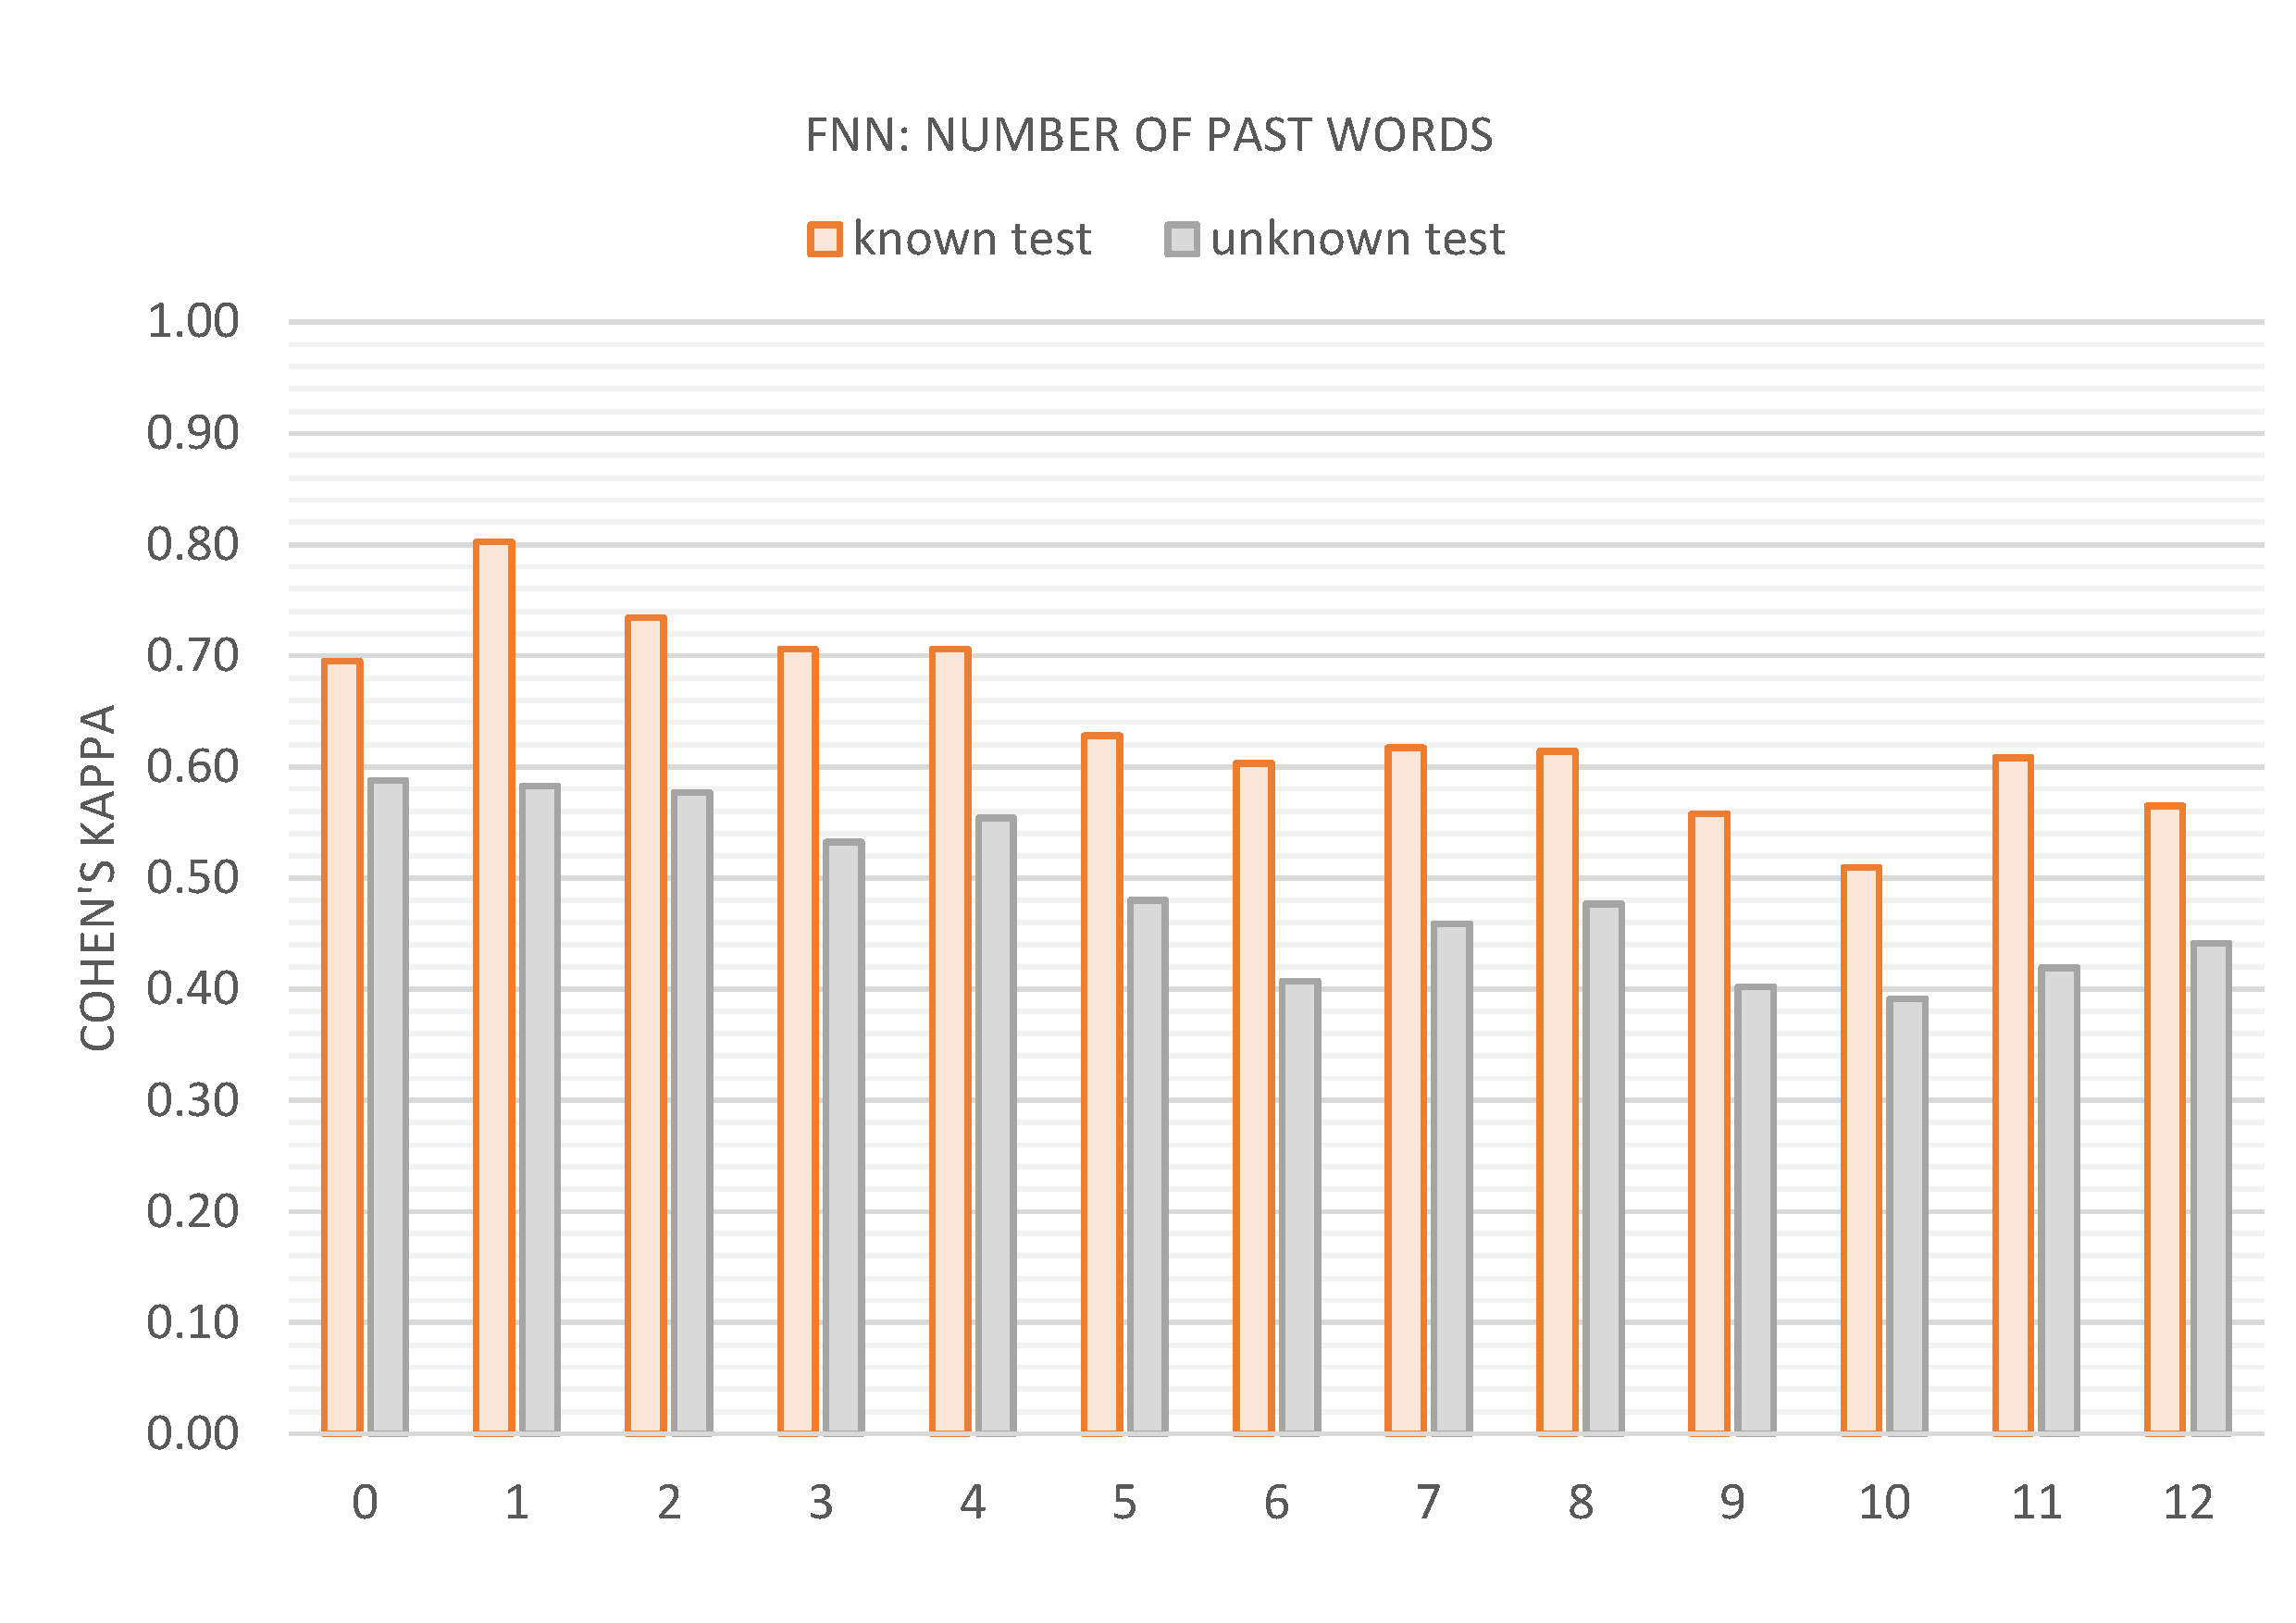
\includegraphics[width=\textwidth]{images/evaluation_fnn_p_k}
	\caption[FNN Evaluation: Number of Past Words]{The evaluation results of the FNN: Cohen's Kappa for parameter $p$: the number of preceding words.}
	\label{f.evaluation.fnn.p.k}
\end{figure}

\vspace{-13mm}
\begin{figure}[H]
	\centering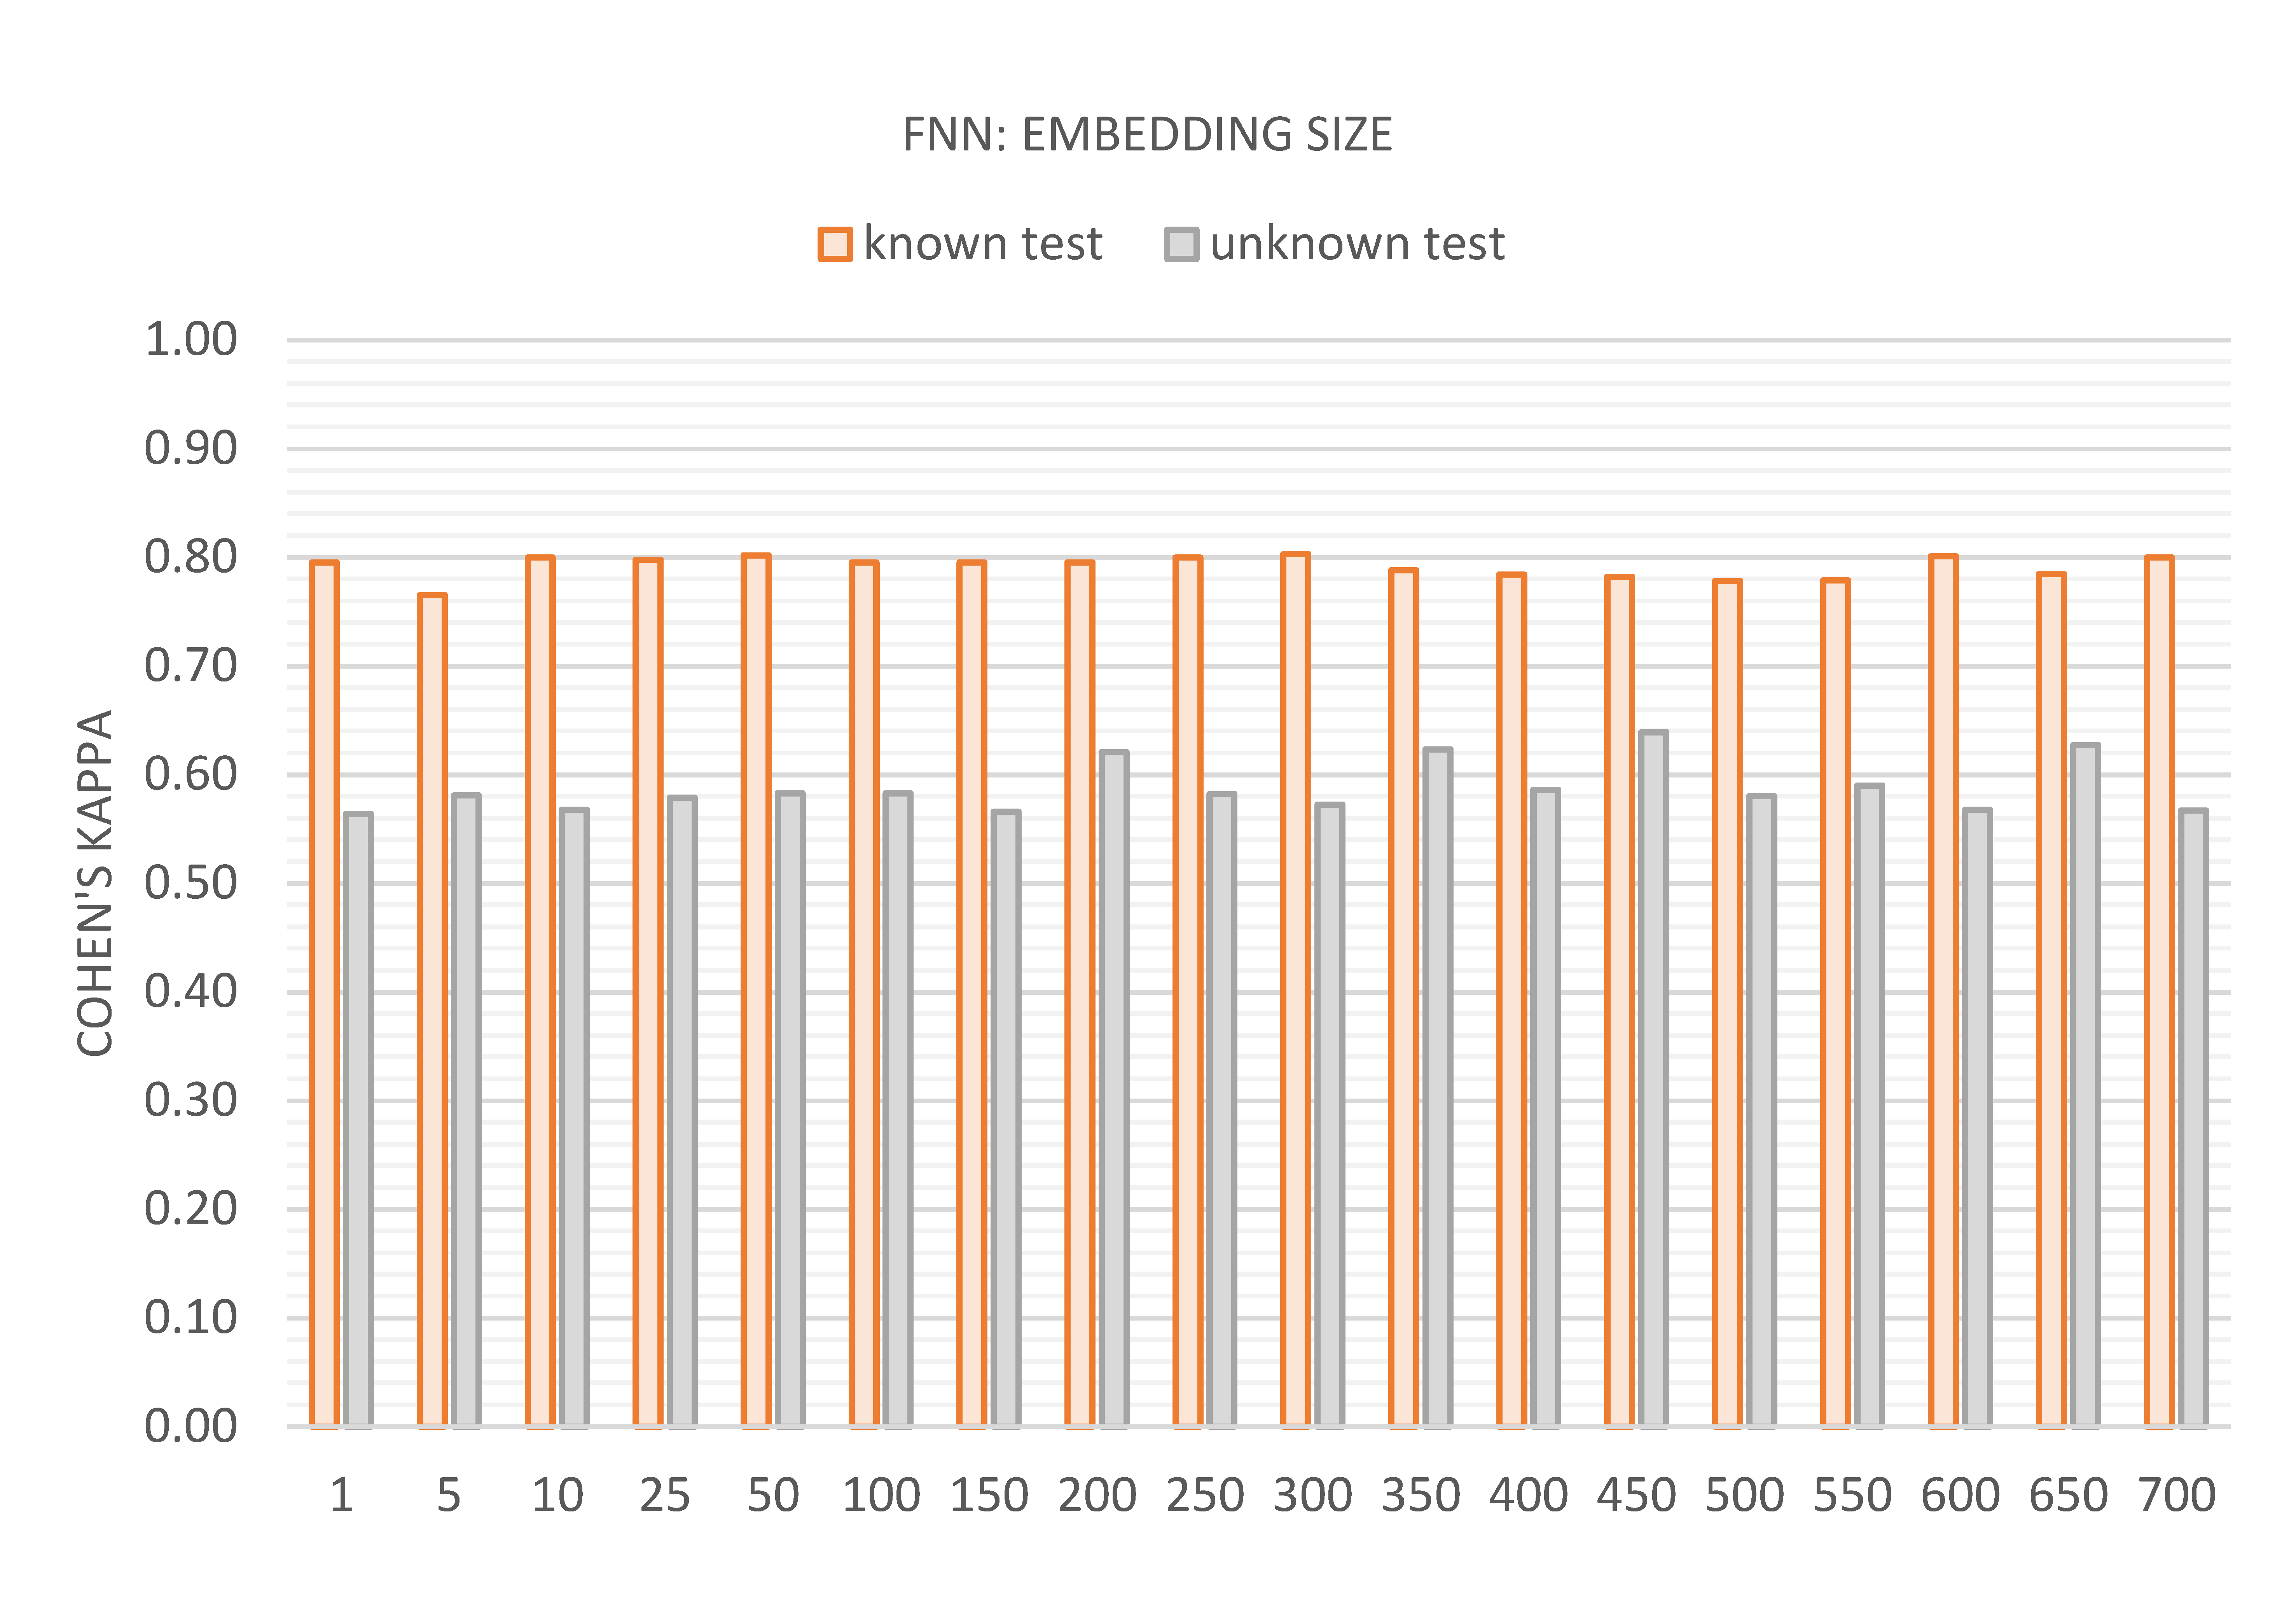
\includegraphics[width=\textwidth]{images/evaluation_fnn_e_k}
	\caption[FNN Evaluation: Number of Past Words]{The evaluation results of the FNN: Cohen's Kappa for parameter $e$: the embedding size.}
	\label{f.evaluation.fnn.e.k}
\end{figure}

\vspace{-11mm}
\begin{figure}[H]
	\centering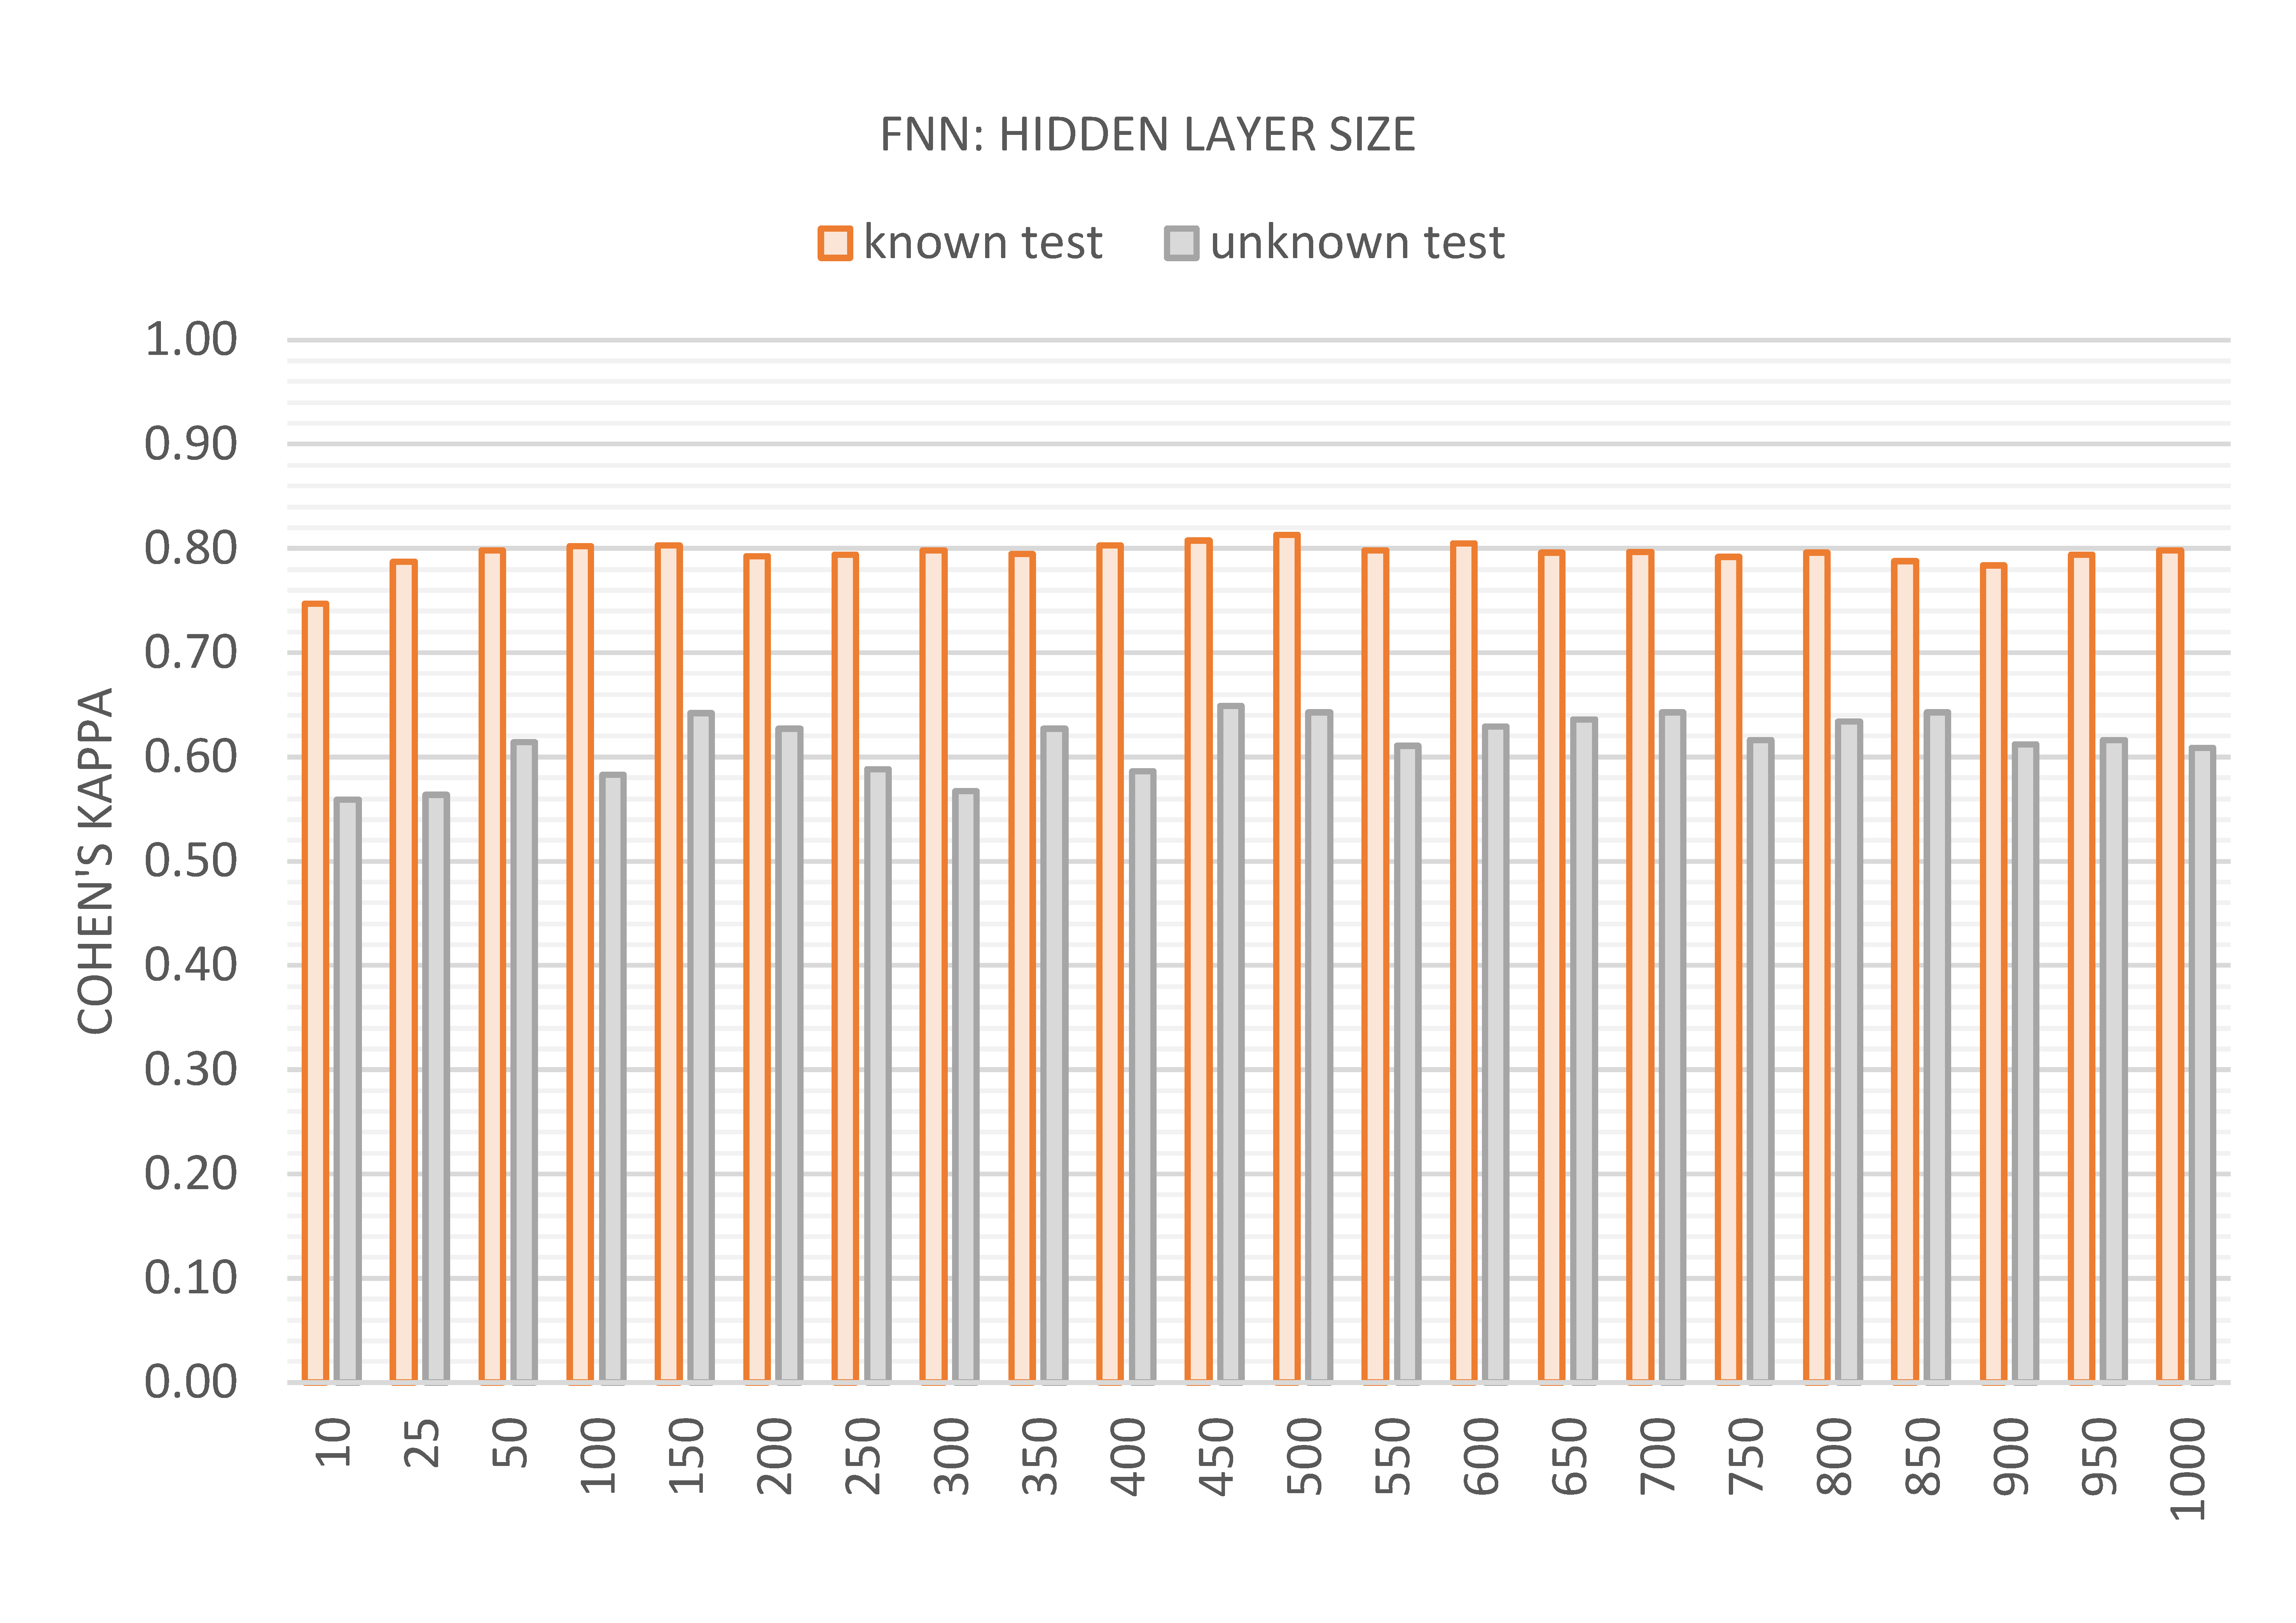
\includegraphics[width=\textwidth]{images/evaluation_fnn_s_k}
	\caption[FNN Evaluation: Hidden Layer Size]{The evaluation results of the FNN: Cohen's Kappa for parameter $s$: the size of the hidden layer.}
	\label{f.evaluation.fnn.s.k}
\end{figure}

\vspace{-11mm}
\begin{figure}[H]
	\centering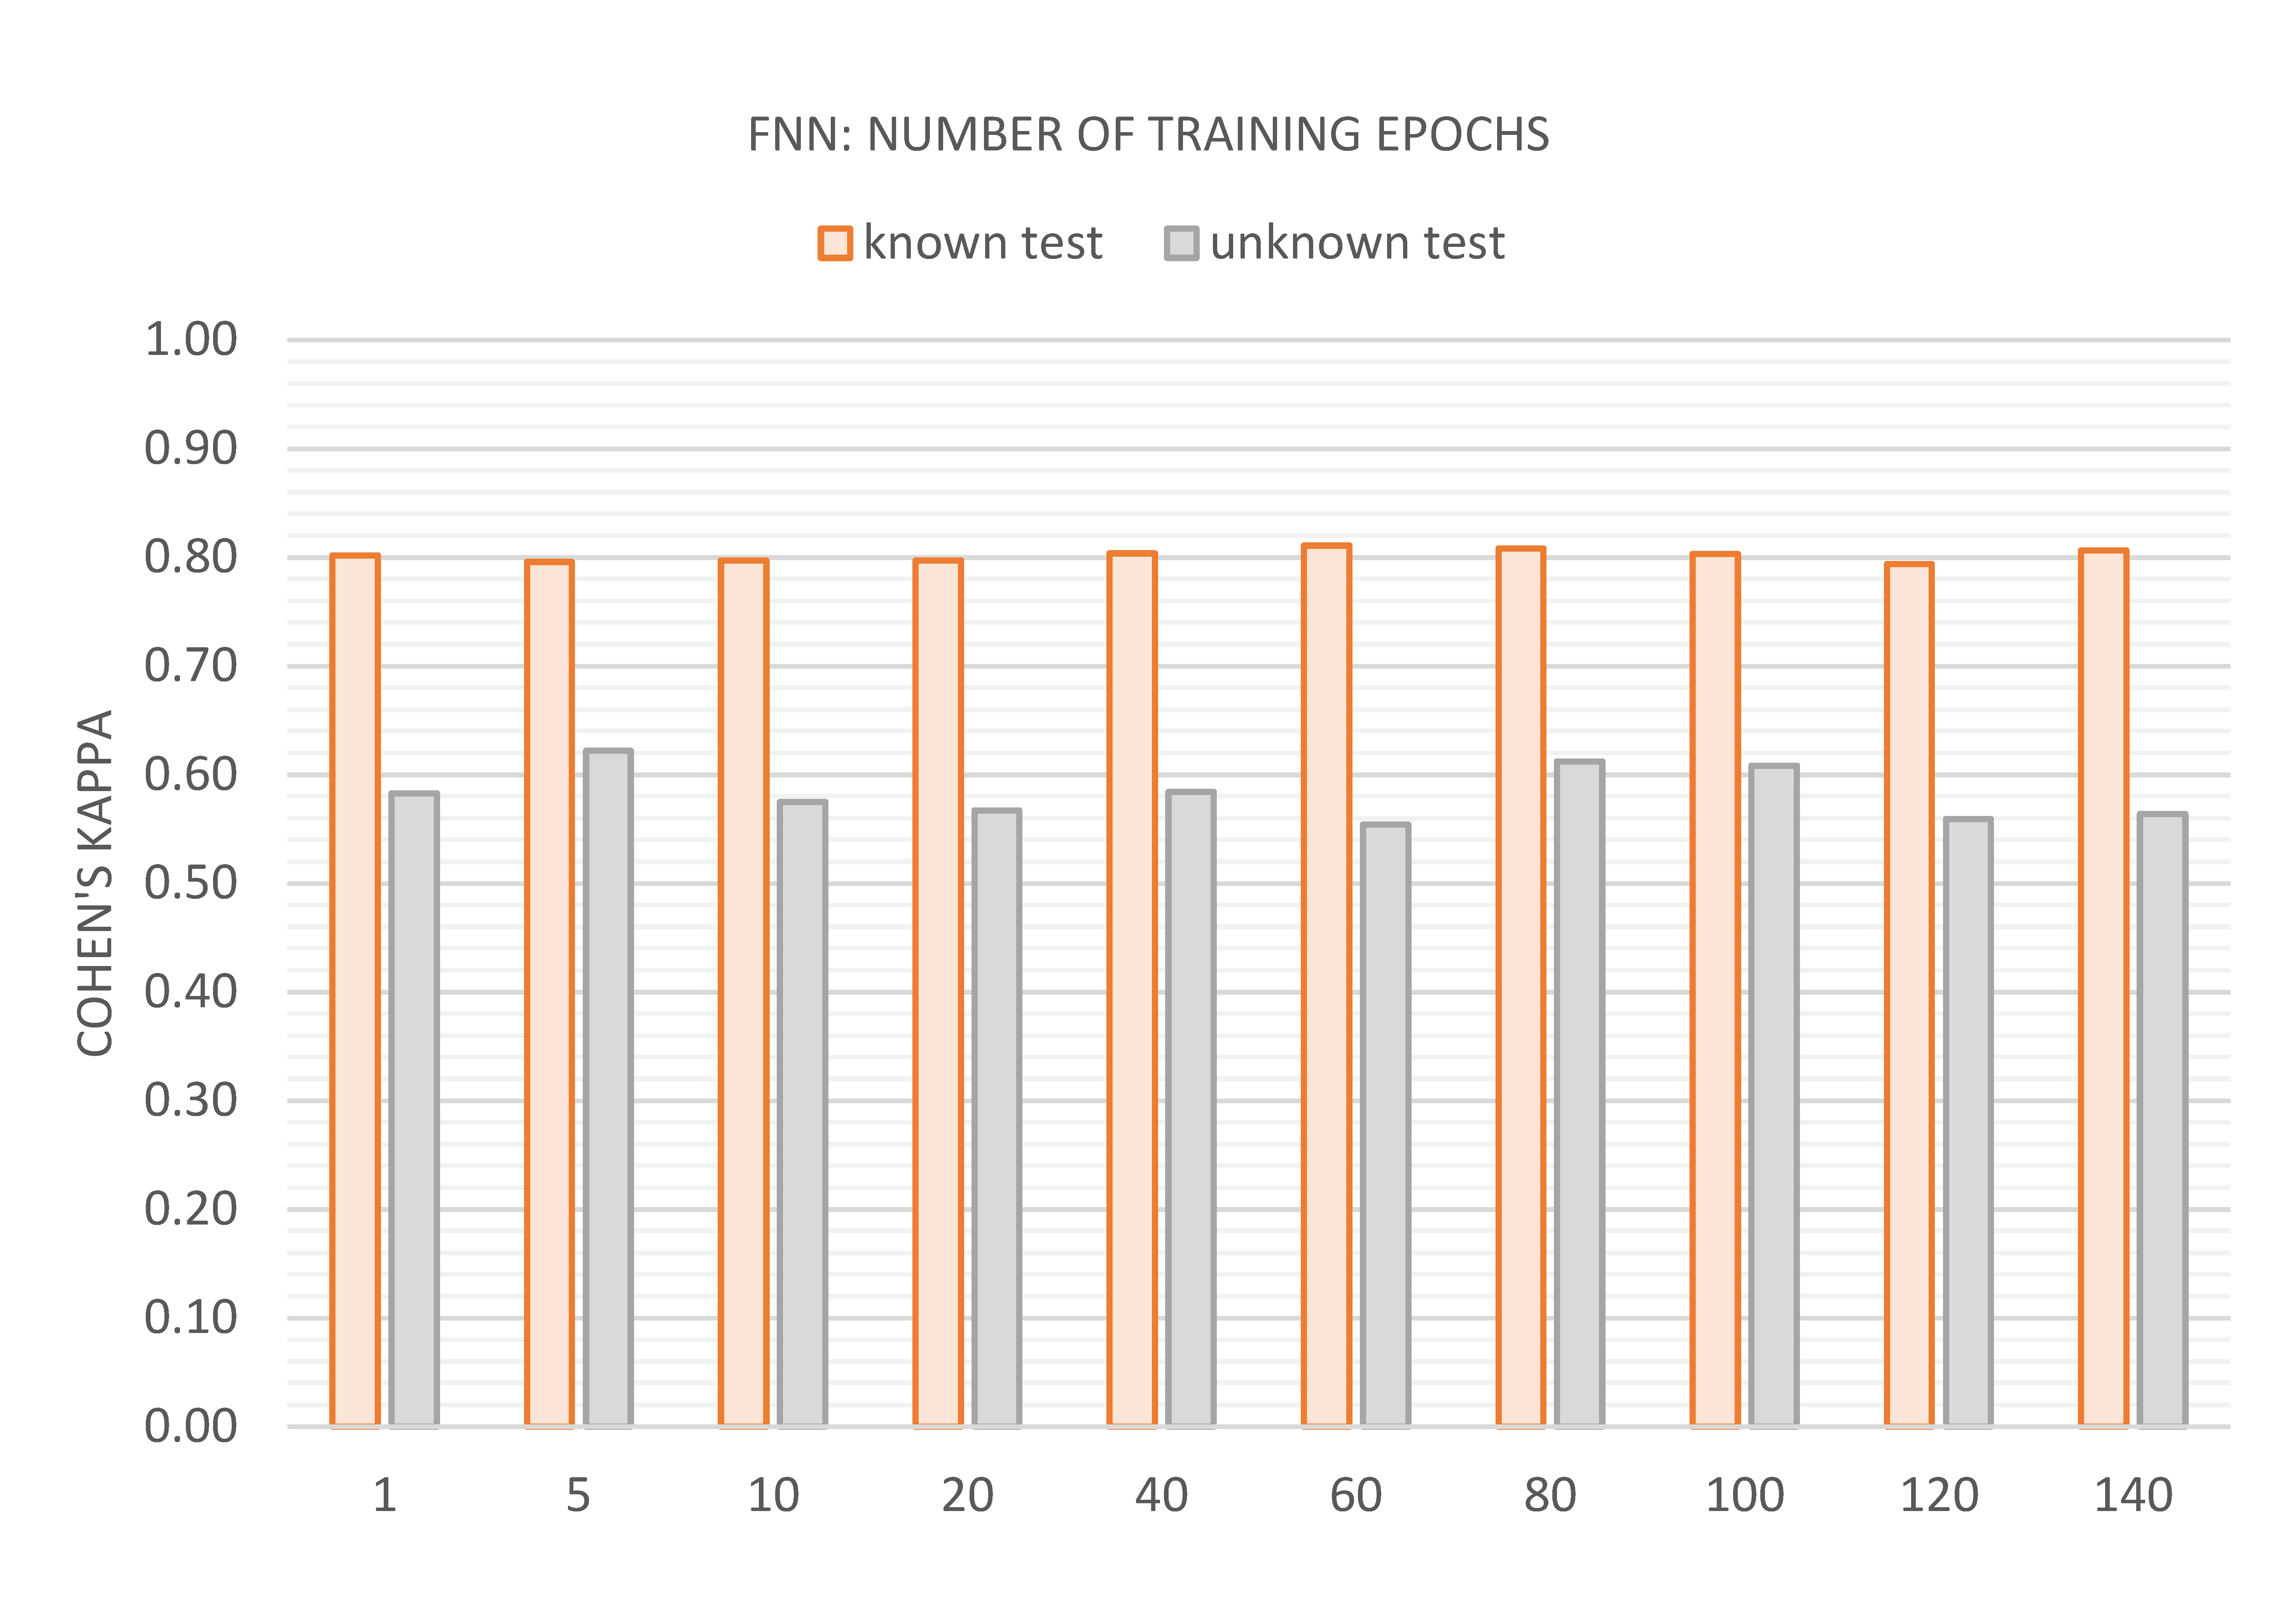
\includegraphics[width=\textwidth]{images/evaluation_fnn_n_k}
	\caption[FNN Evaluation: Number of Training Epochs]{The evaluation results of the FNN: Cohen's Kappa for parameter $n$: the number of training epochs.}
	\label{f.evaluation.fnn.n.k}
\end{figure}

\vspace{-11mm}
\begin{figure}[H]
	\centering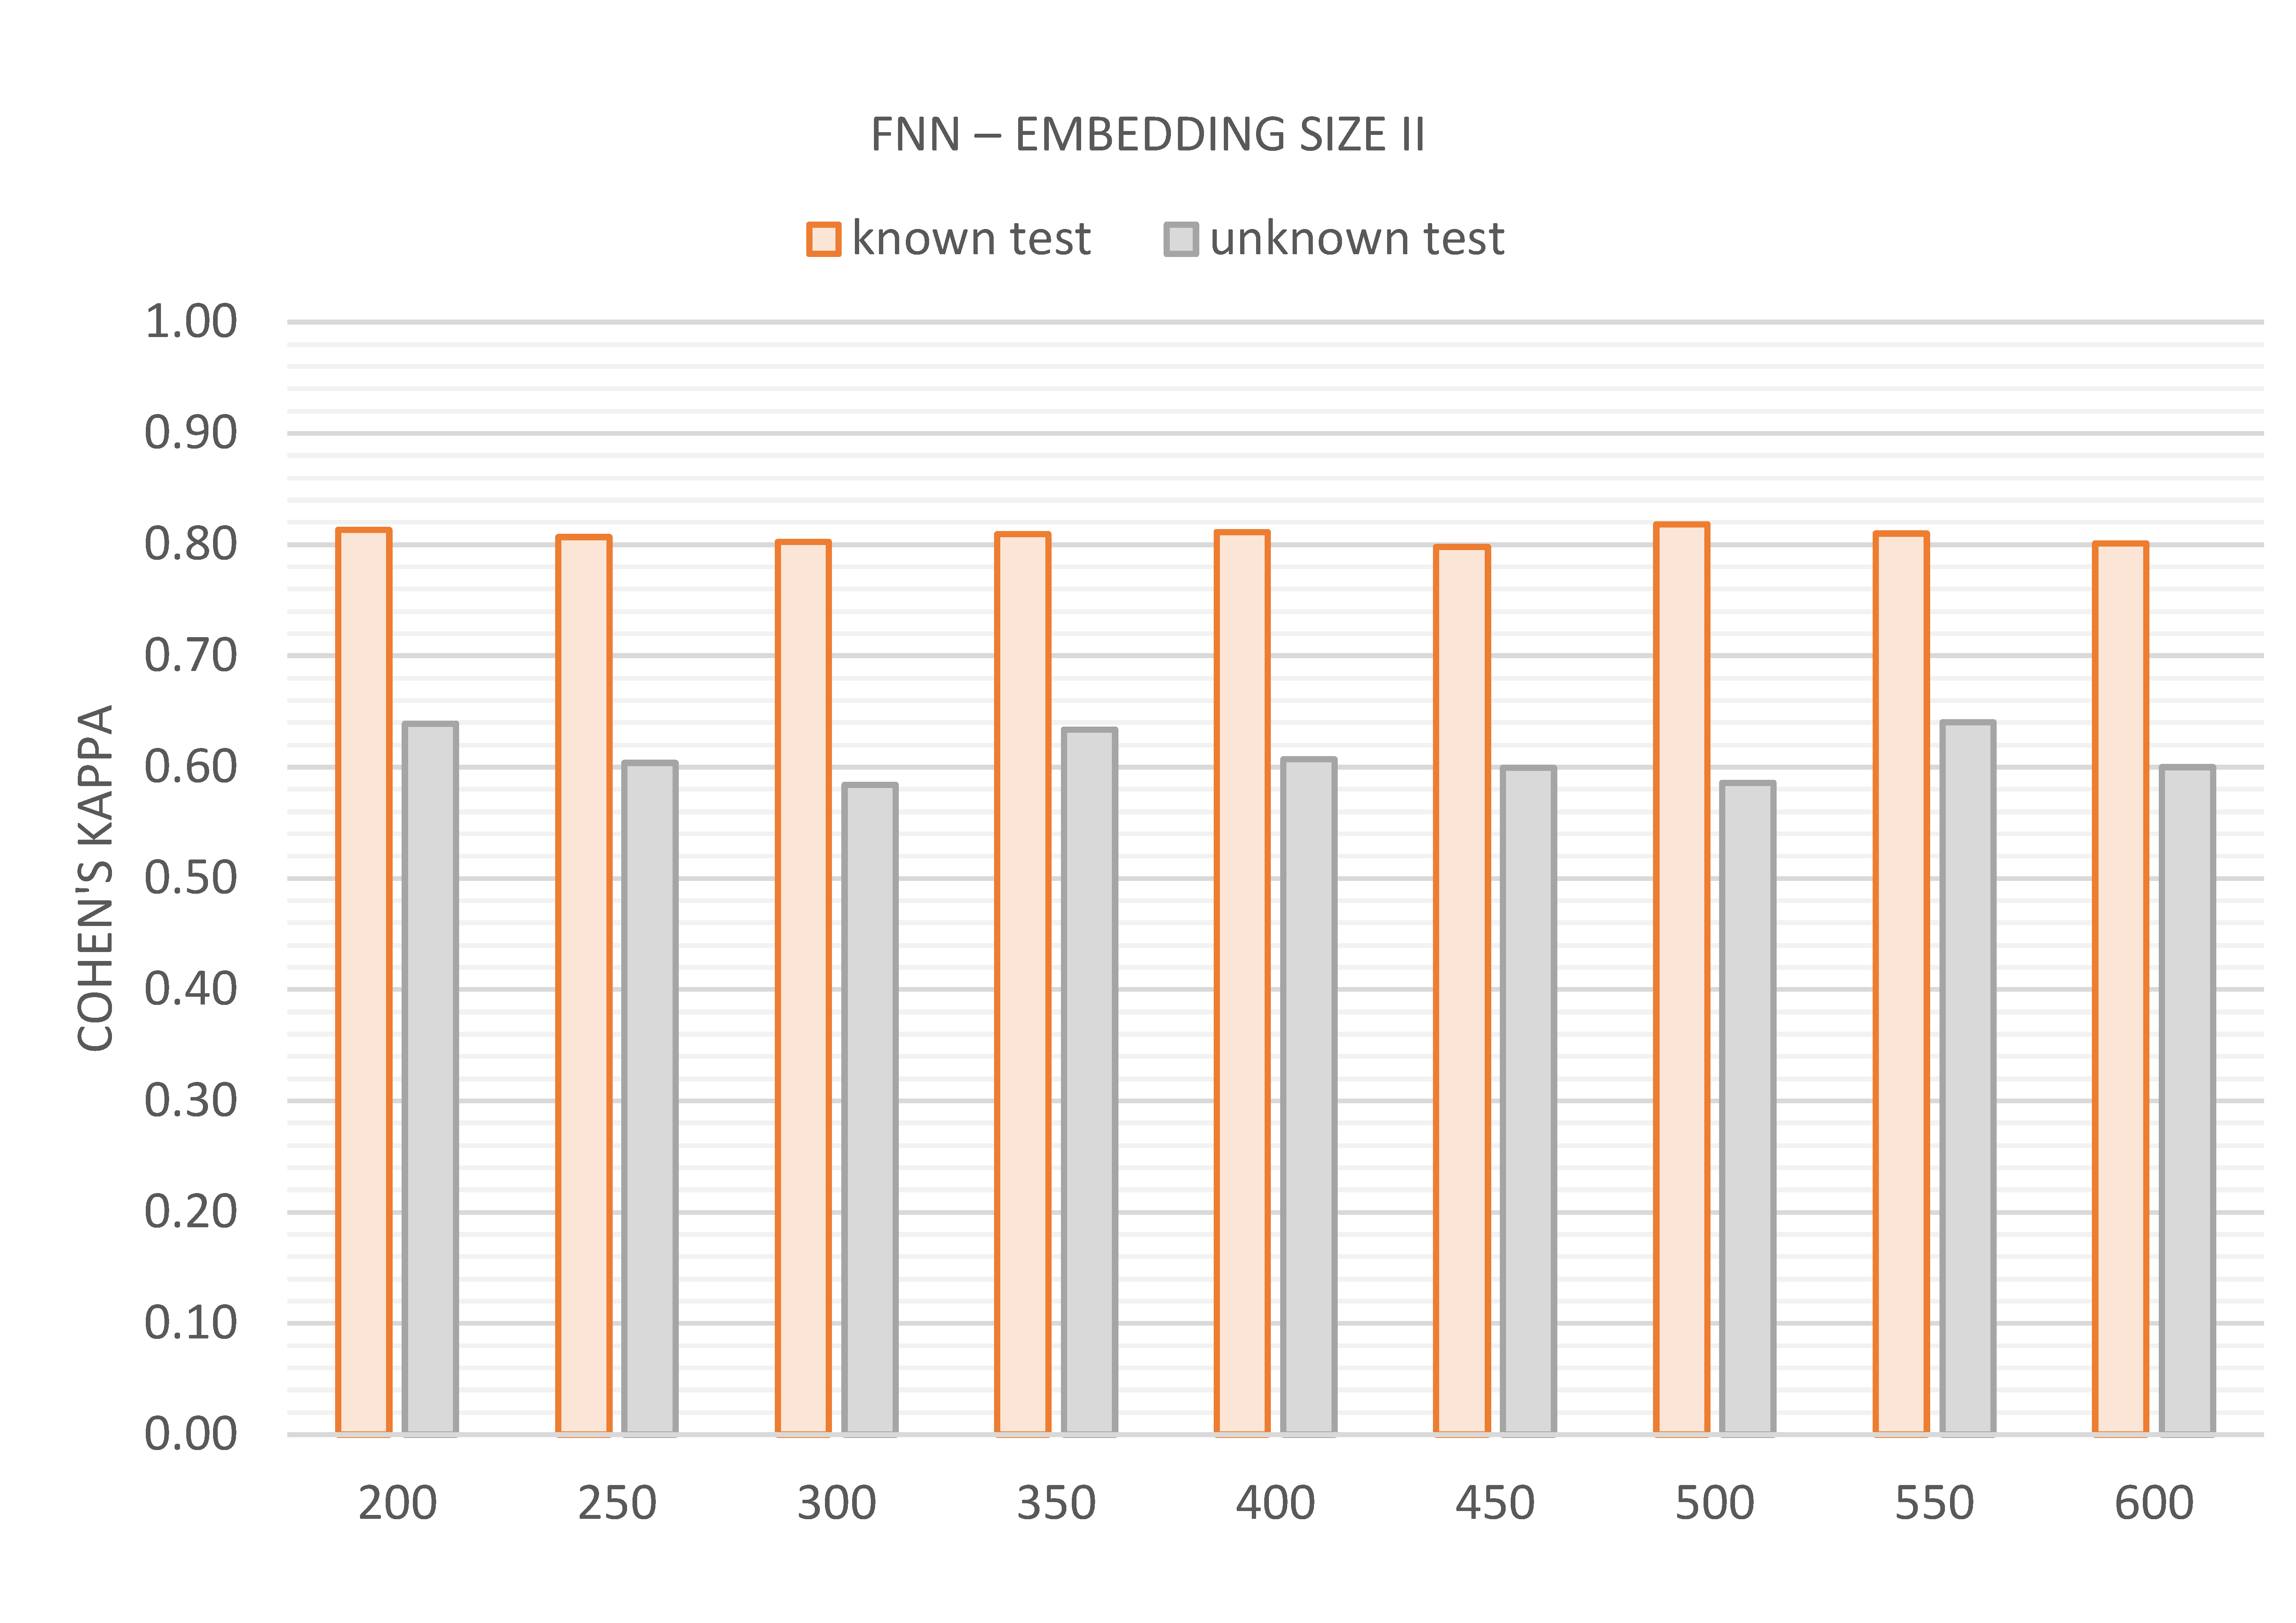
\includegraphics[width=\textwidth]{images/evaluation_fnn_e2_k}
	\caption[FNN Evaluation: Number of Training Epochs]{The evaluation results of the FNN: Cohen's Kappa for parameter $n$: the number of training epochs.}
	\label{f.evaluation.fnn.e2.k}
\end{figure}

\vspace{-11mm}
\begin{figure}[H]
	\centering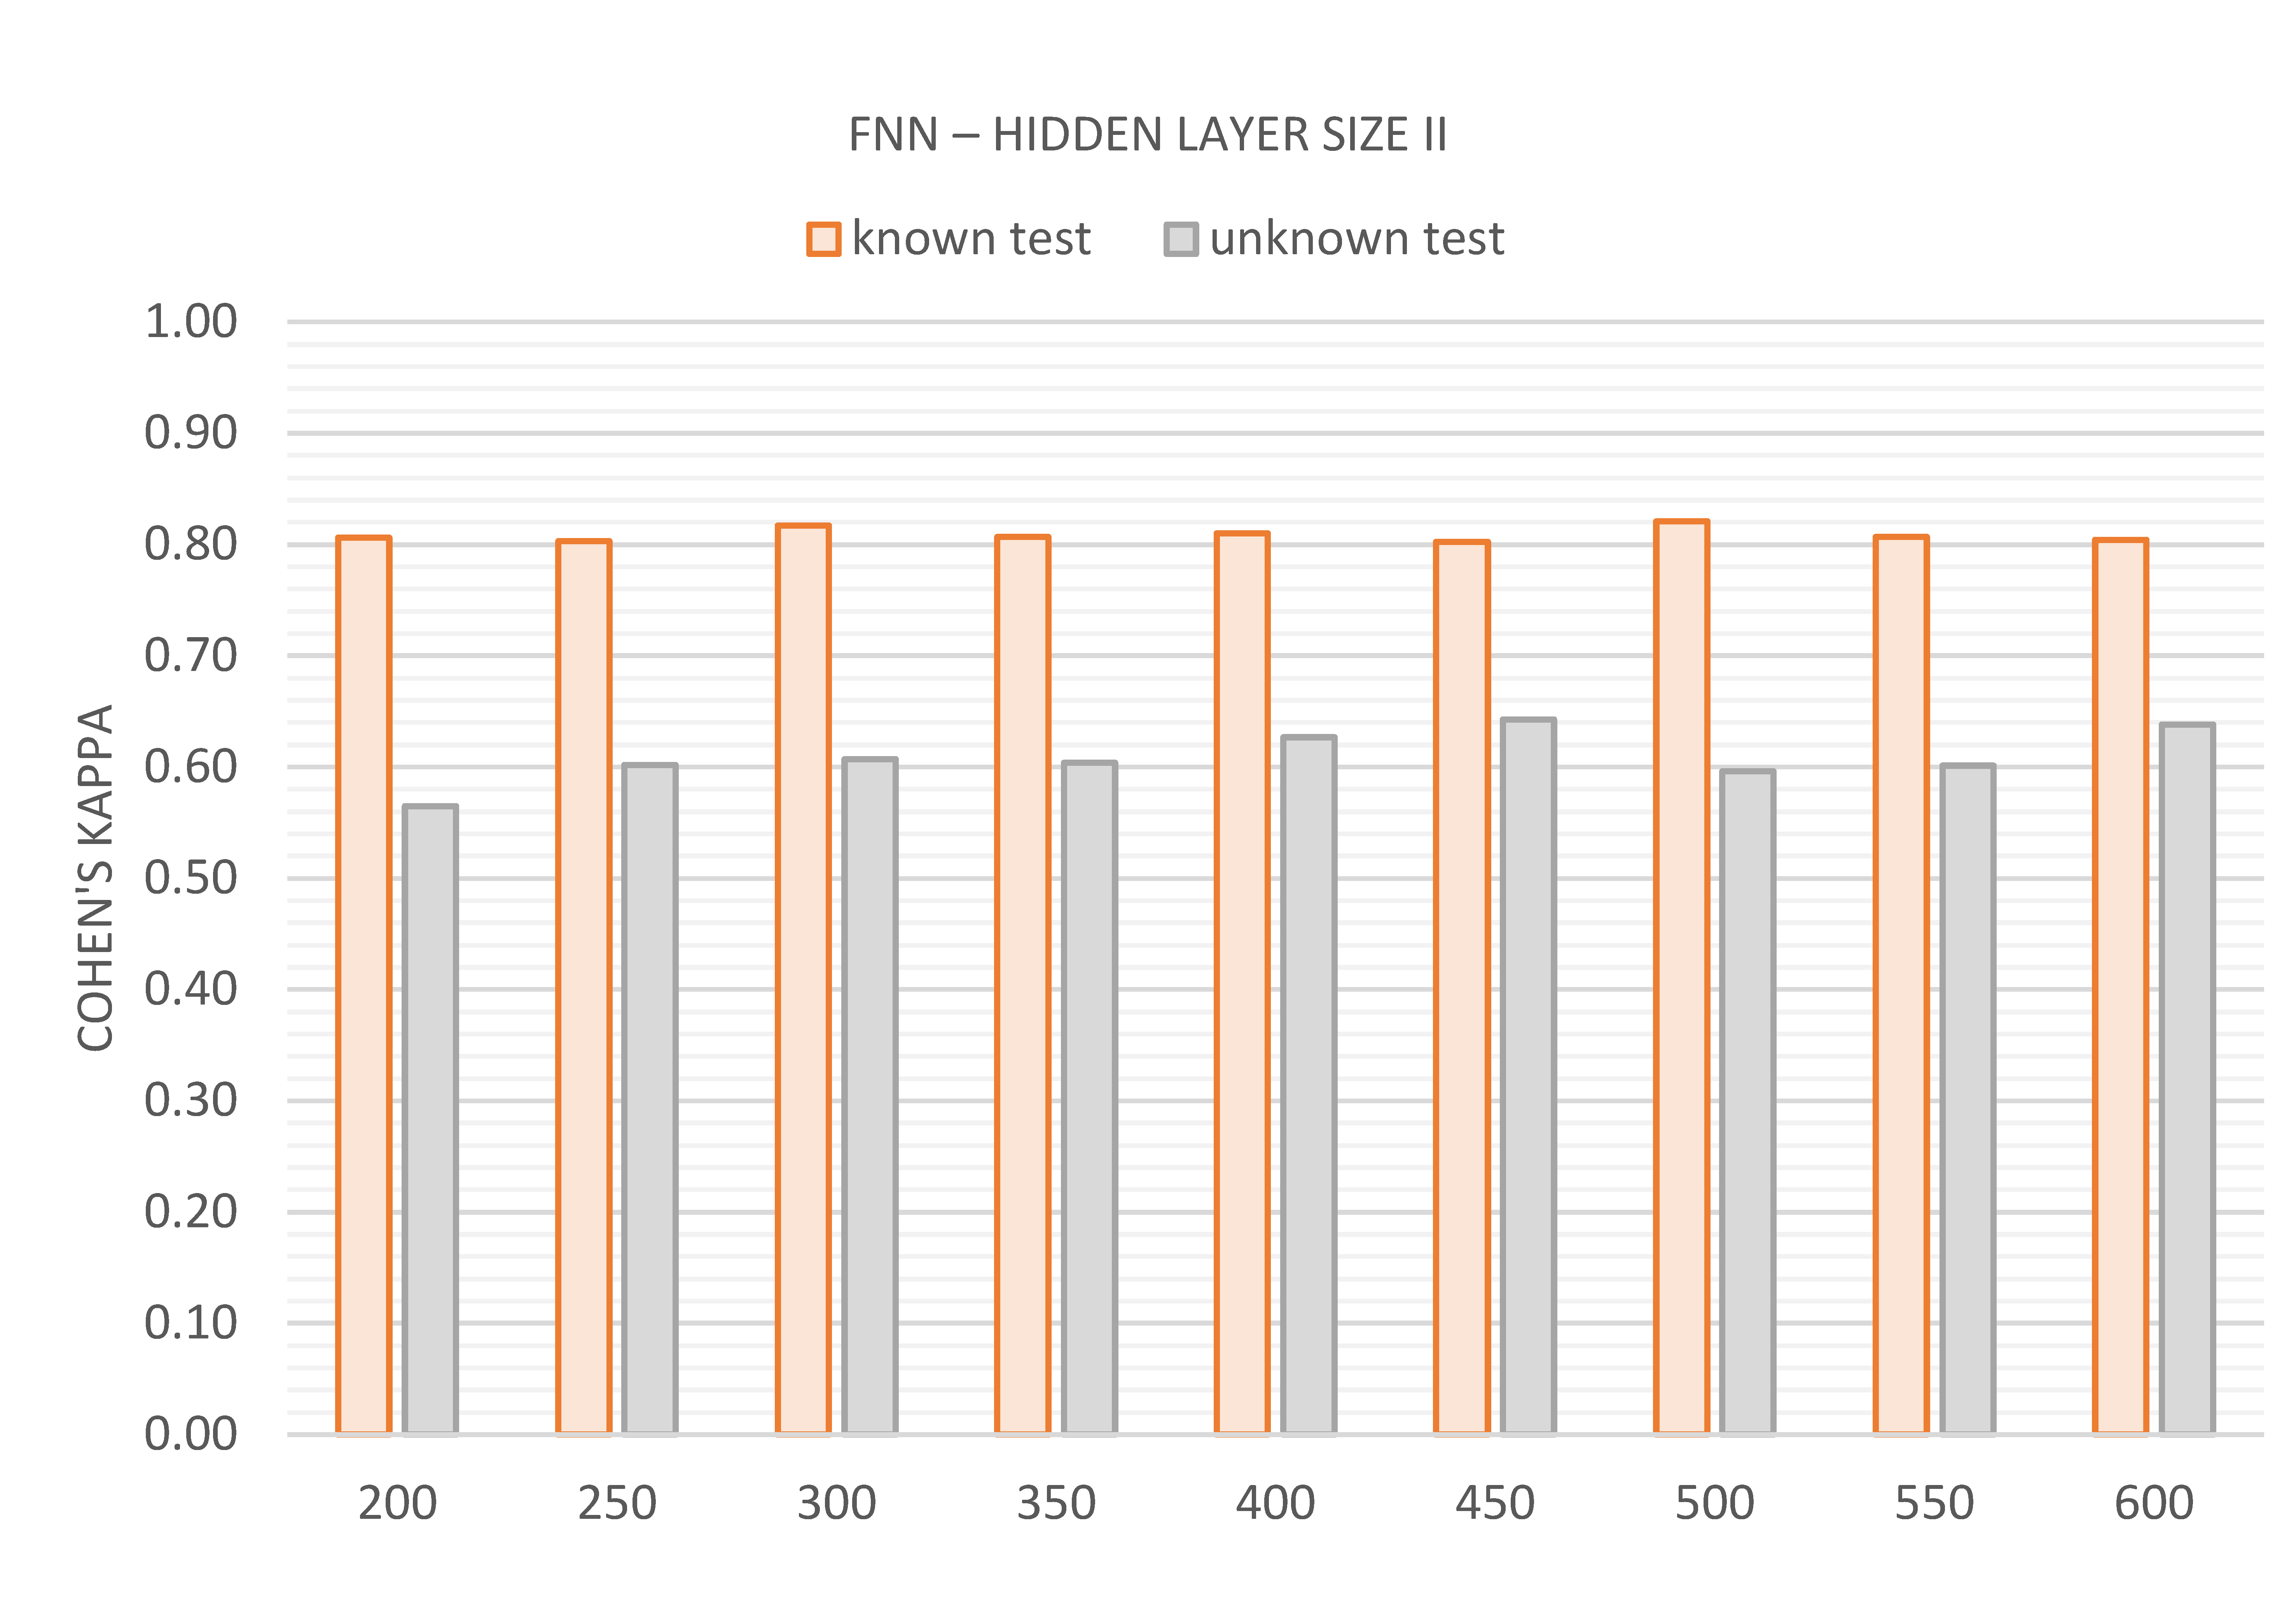
\includegraphics[width=\textwidth]{images/evaluation_fnn_s2_k}
	\caption[FNN Evaluation: Number of Training Epochs]{The evaluation results of the FNN: Cohen's Kappa for parameter $n$: the number of training epochs.}
	\label{f.evaluation.fnn.s2.k}
\end{figure}

\vspace{-11mm}
\begin{figure}[H]
	\centering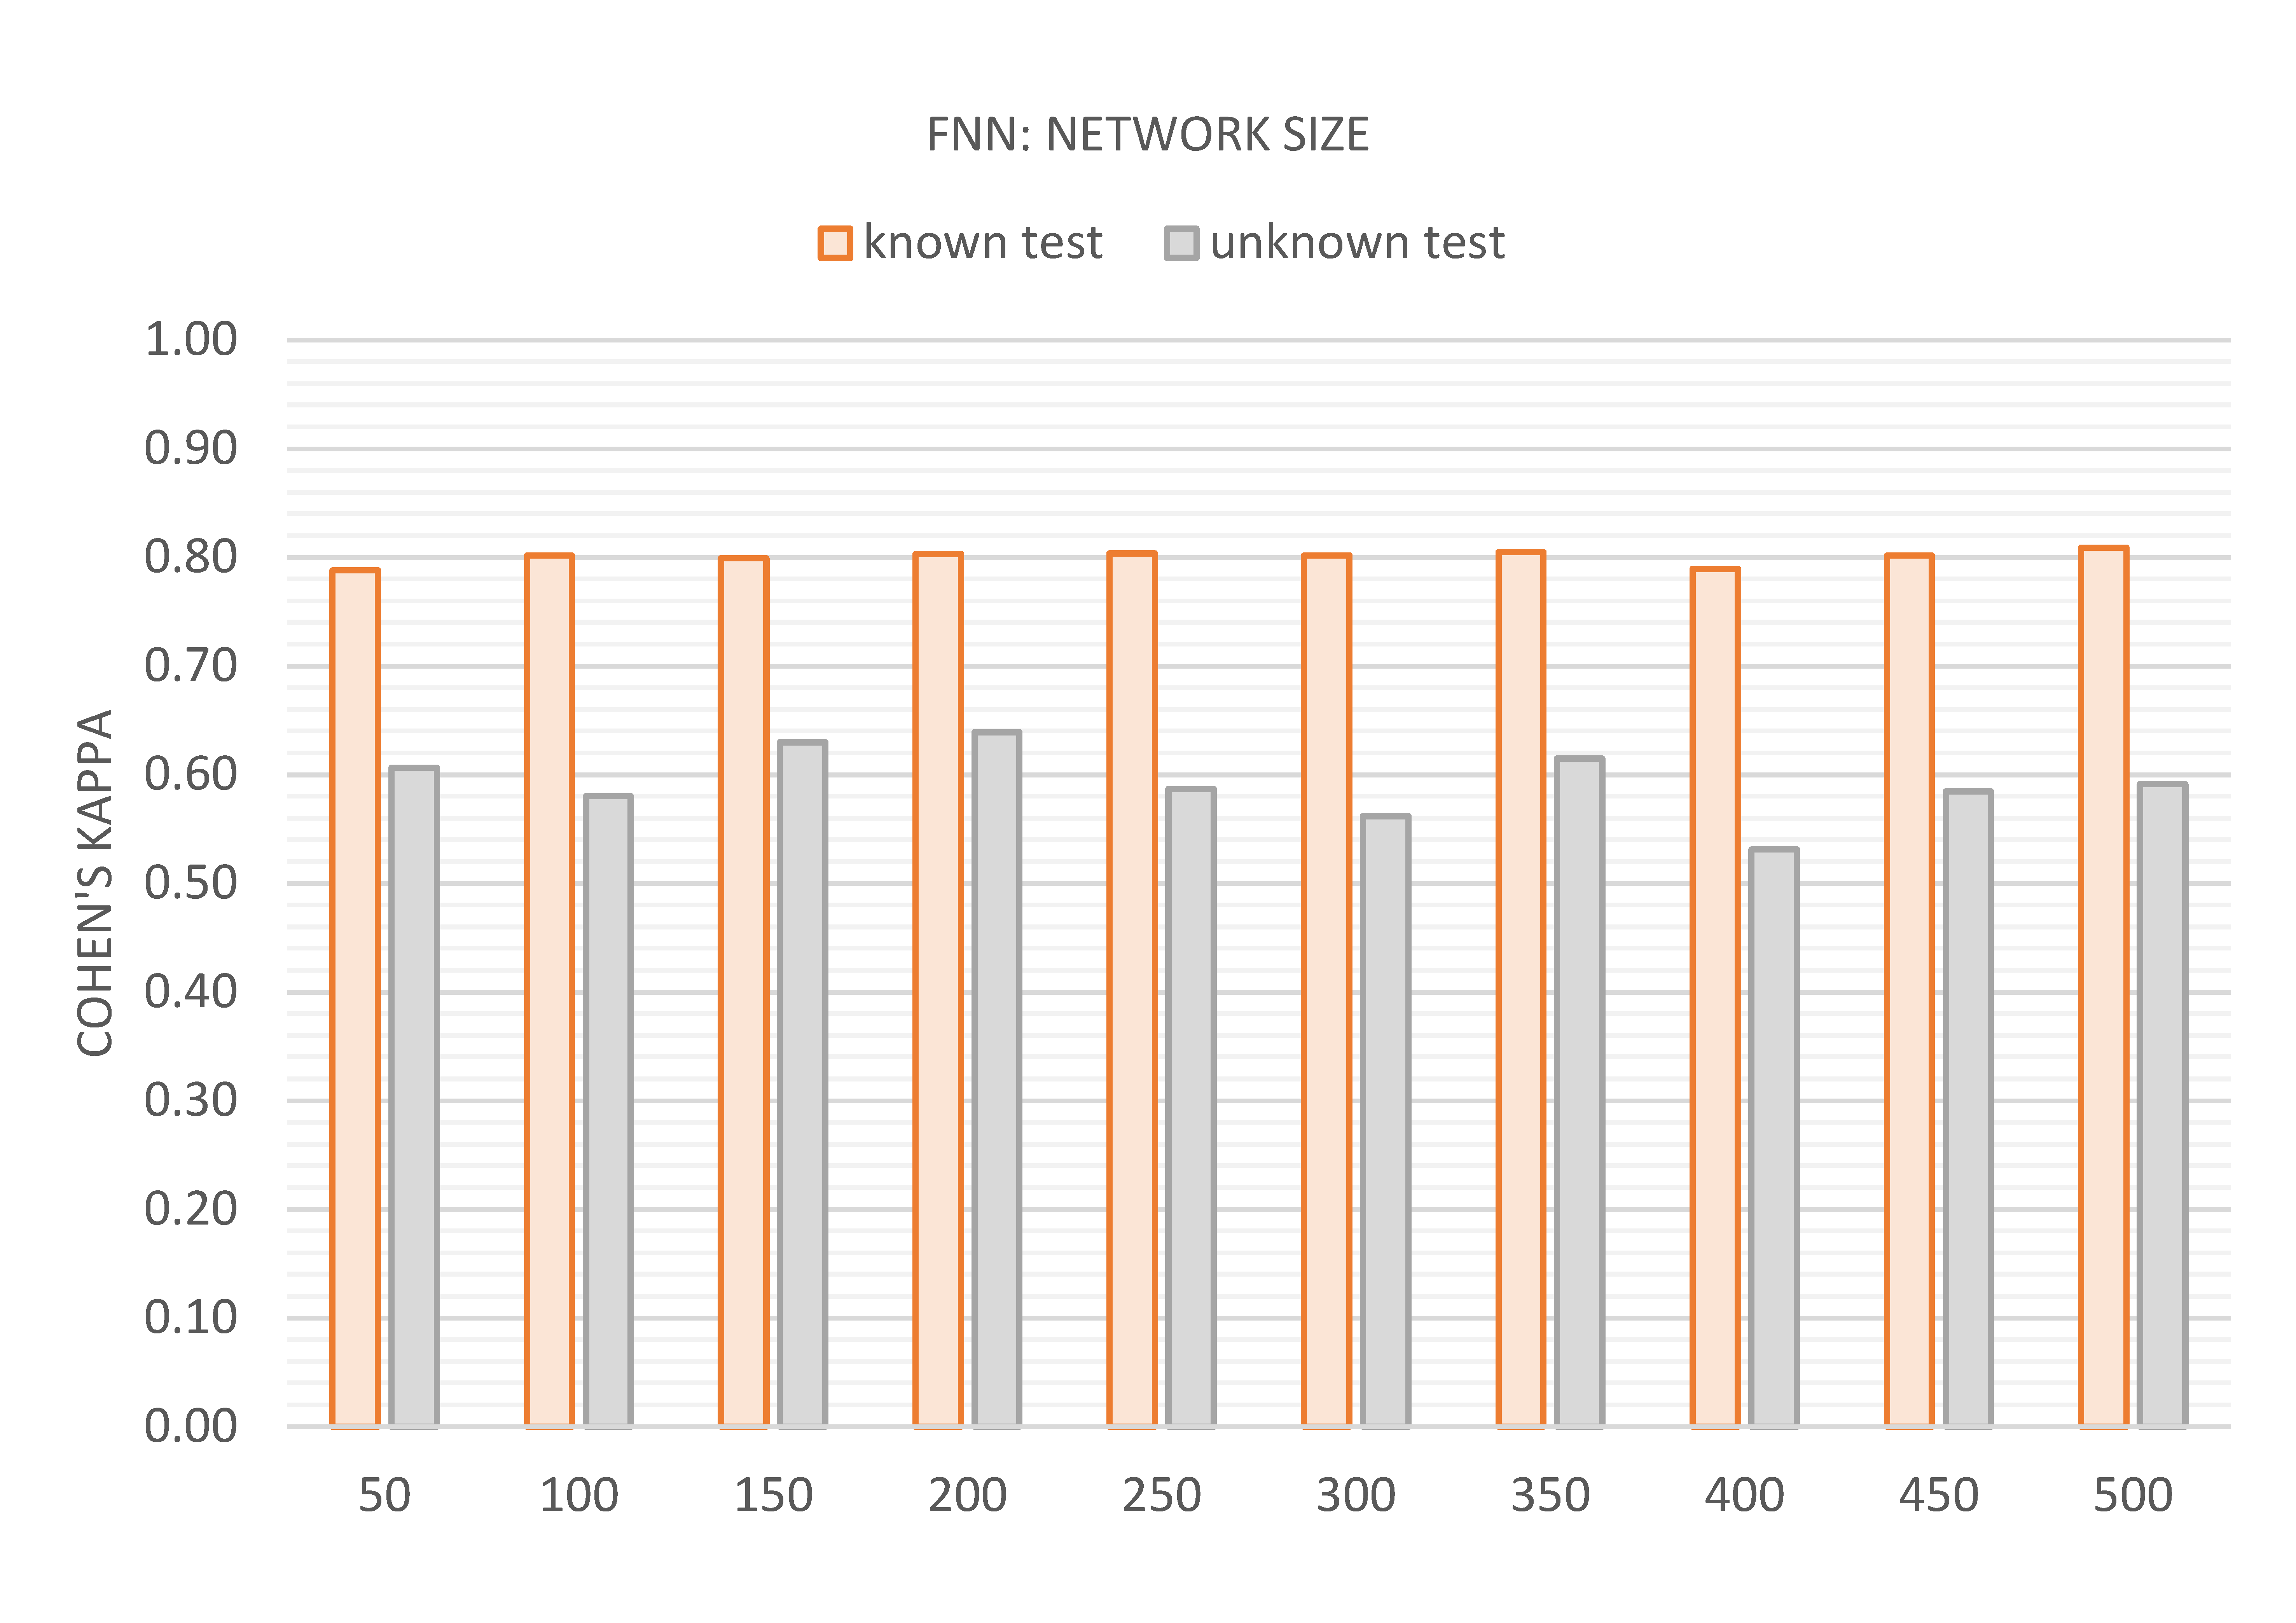
\includegraphics[width=\textwidth]{images/evaluation_fnn_es_k}
	\caption[FNN Evaluation: Network Size]{The evaluation results of the FNN: Cohen's Kappa for uniform scaling of parameters $e$ ad $s$, increasing the whole network size.}
	\label{f.evaluation.fnn.es.k}
\end{figure}

\vspace{-11mm}
\begin{figure}[H]
	\centering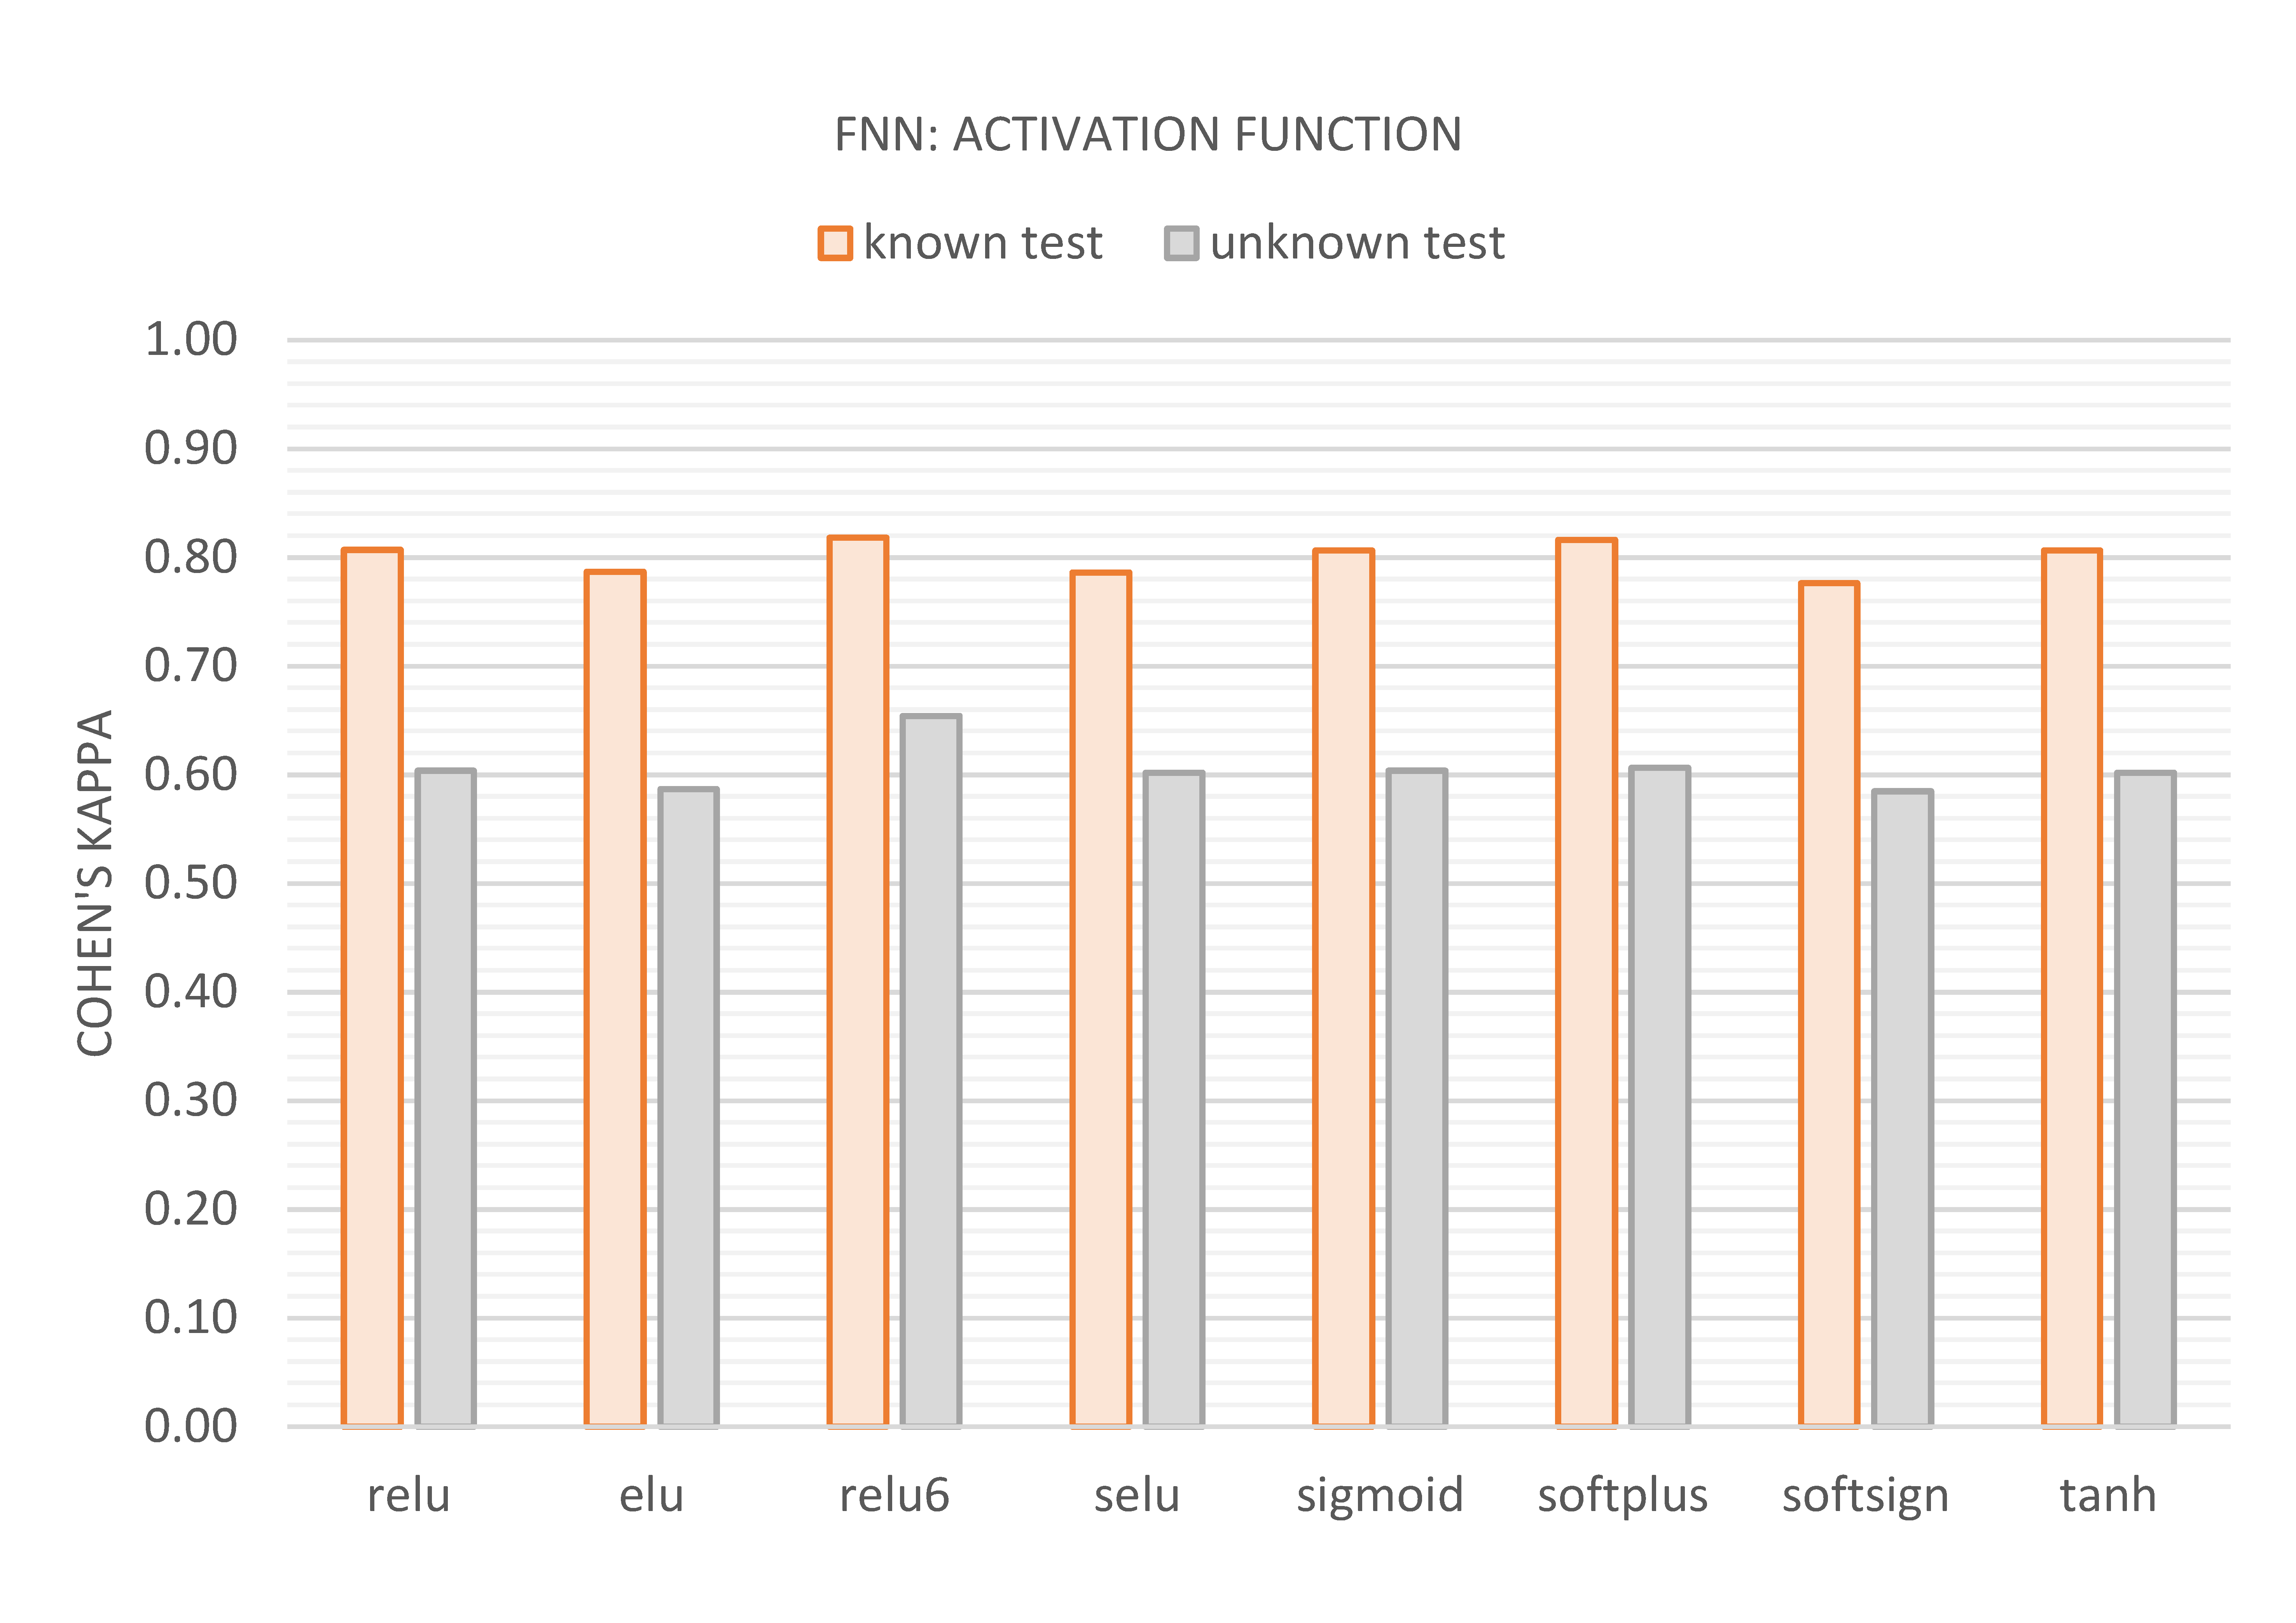
\includegraphics[width=\textwidth]{images/evaluation_fnn_a_k}
	\caption[FNN Evaluation: Number of Training Epochs]{The evaluation results of the FNN: Cohen's Kappa for parameter $n$: the number of training epochs.}
	\label{f.evaluation.fnn.a.k}
\end{figure}

\newpage

\section{RNN Evaluation: Cohen's Kappa}\label{c.appendix.kappa.rnn}
\vspace{-13mm}
\begin{figure}[H]
	\centering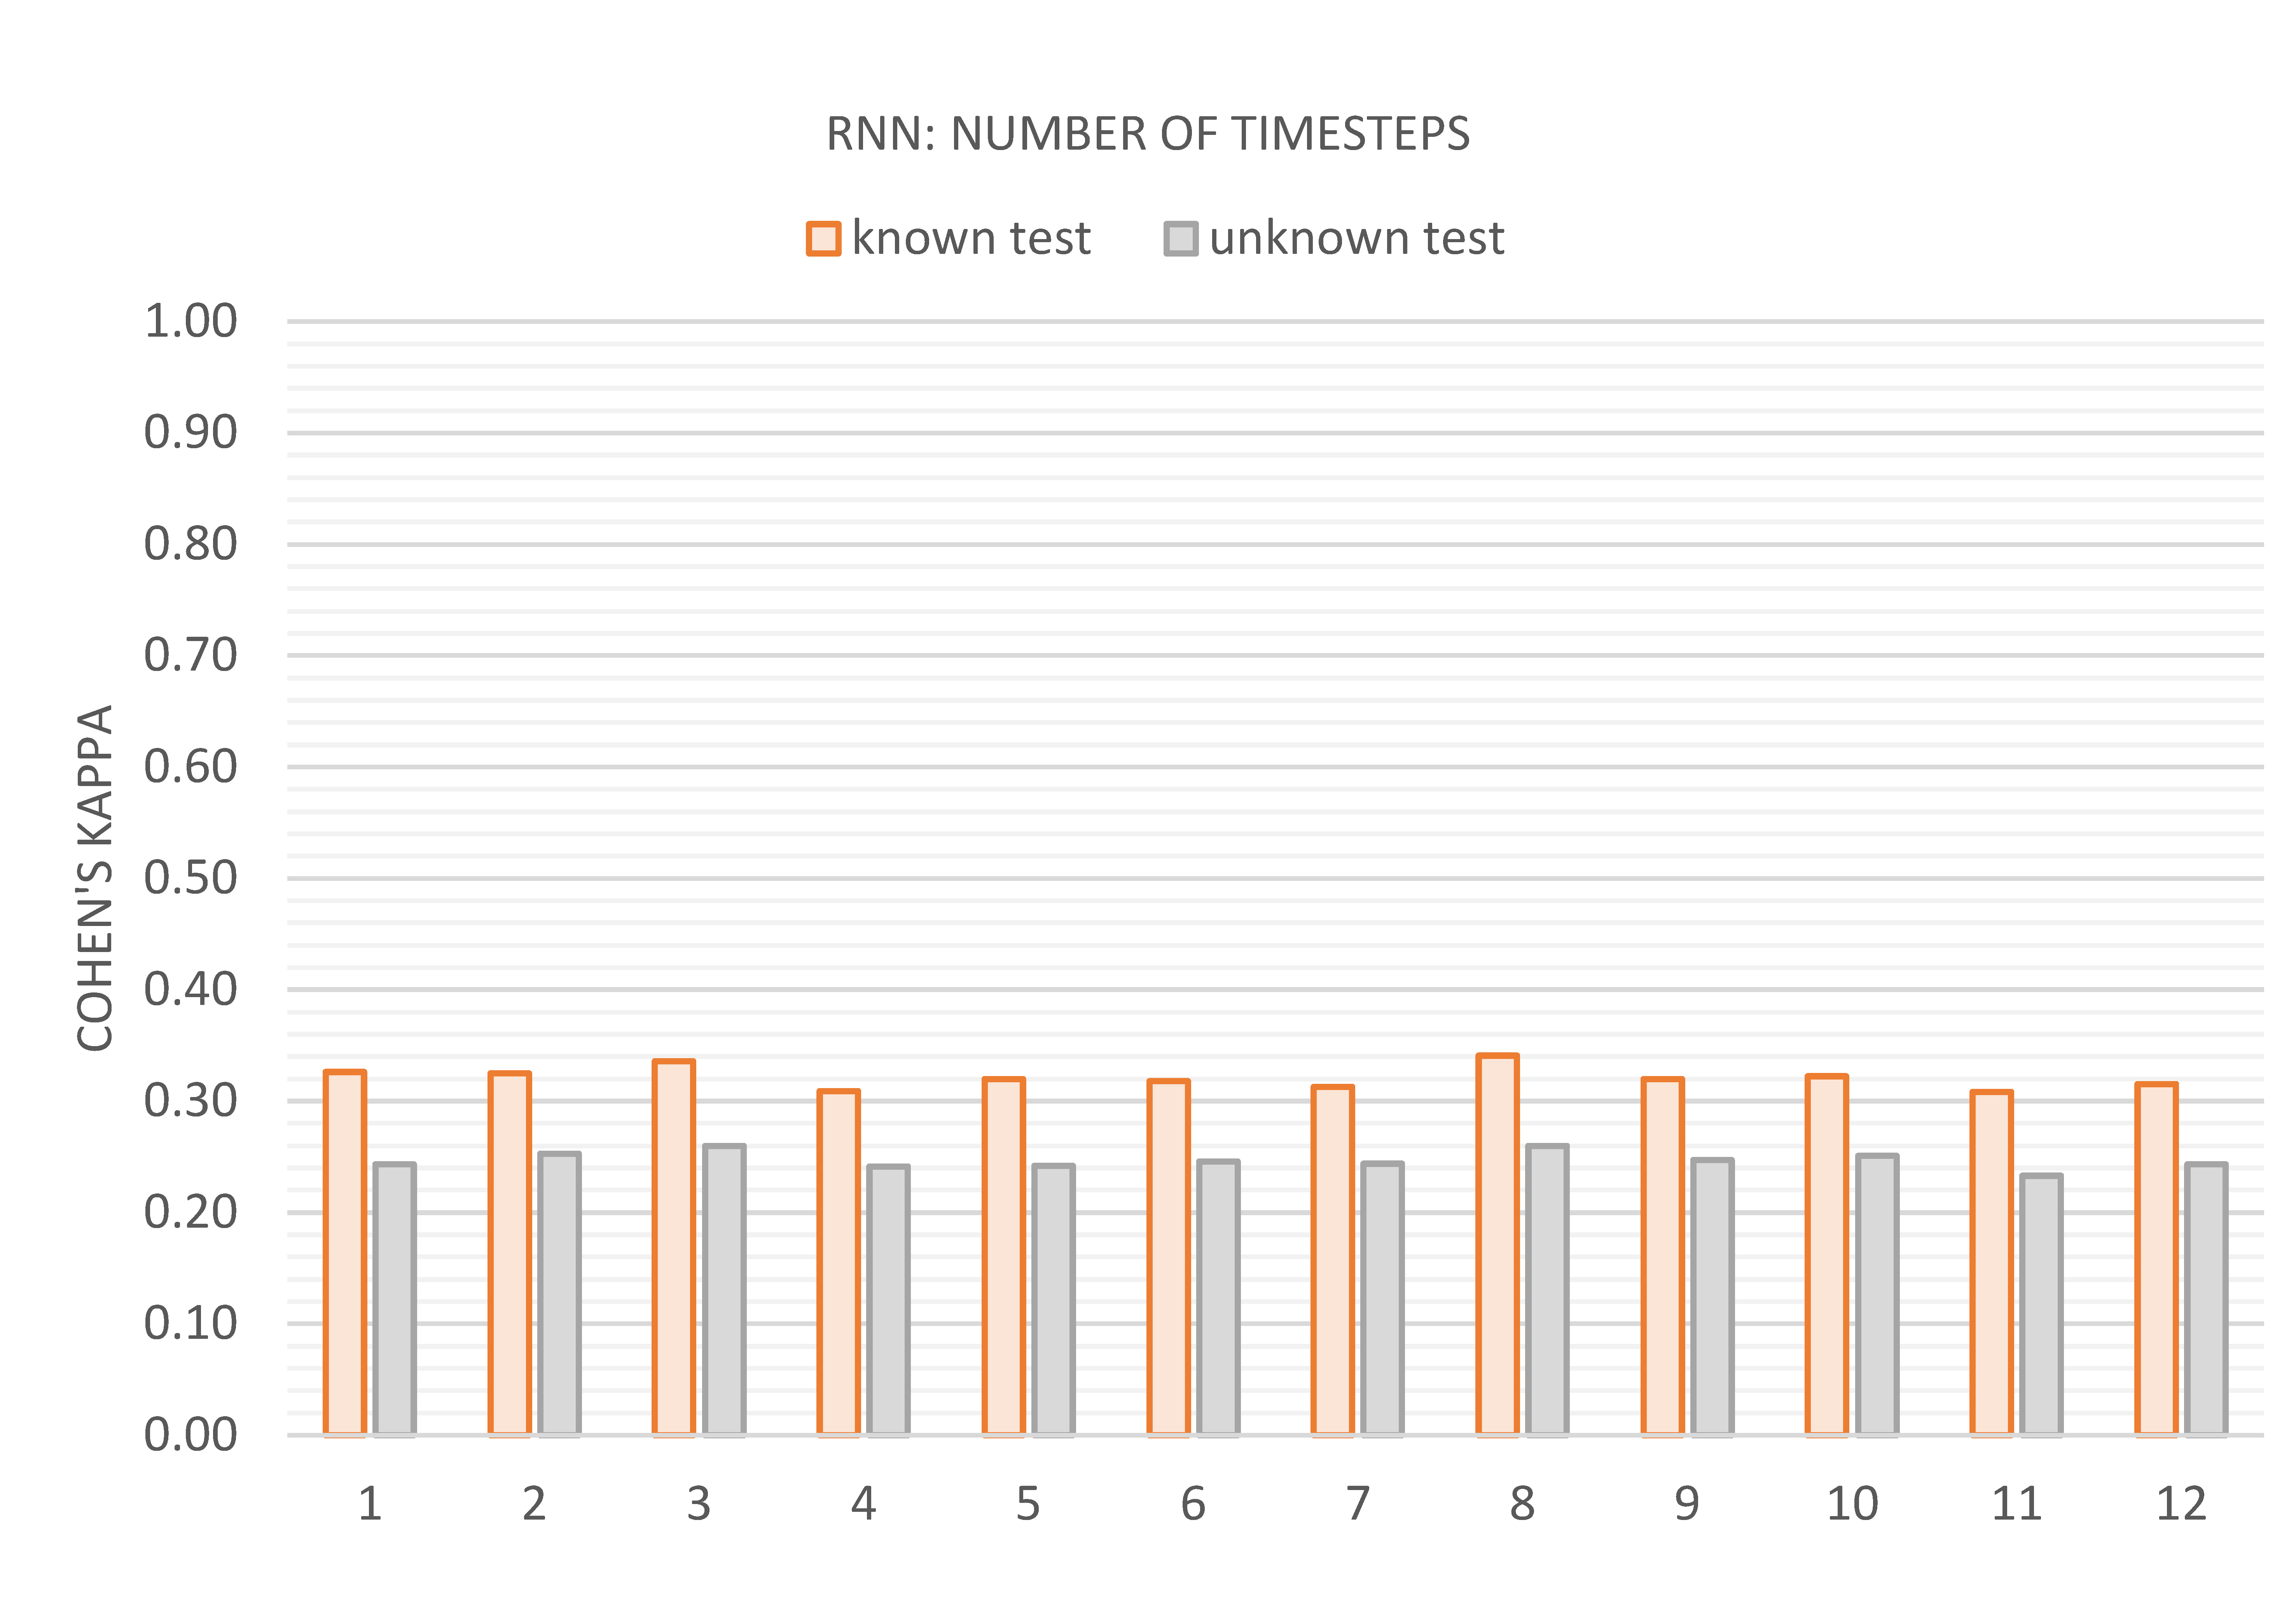
\includegraphics[width=\textwidth]{images/evaluation_rnn_t_k}
	\caption[RNN Evaluation: Number of Time Steps]{The evaluation results of the RNN: Cohen's Kappa for parameter $t$: the number of time steps.}
	\label{f.evaluation.rnn.t.k}
\end{figure}

\vspace{-13mm}
\begin{figure}[H]
	\centering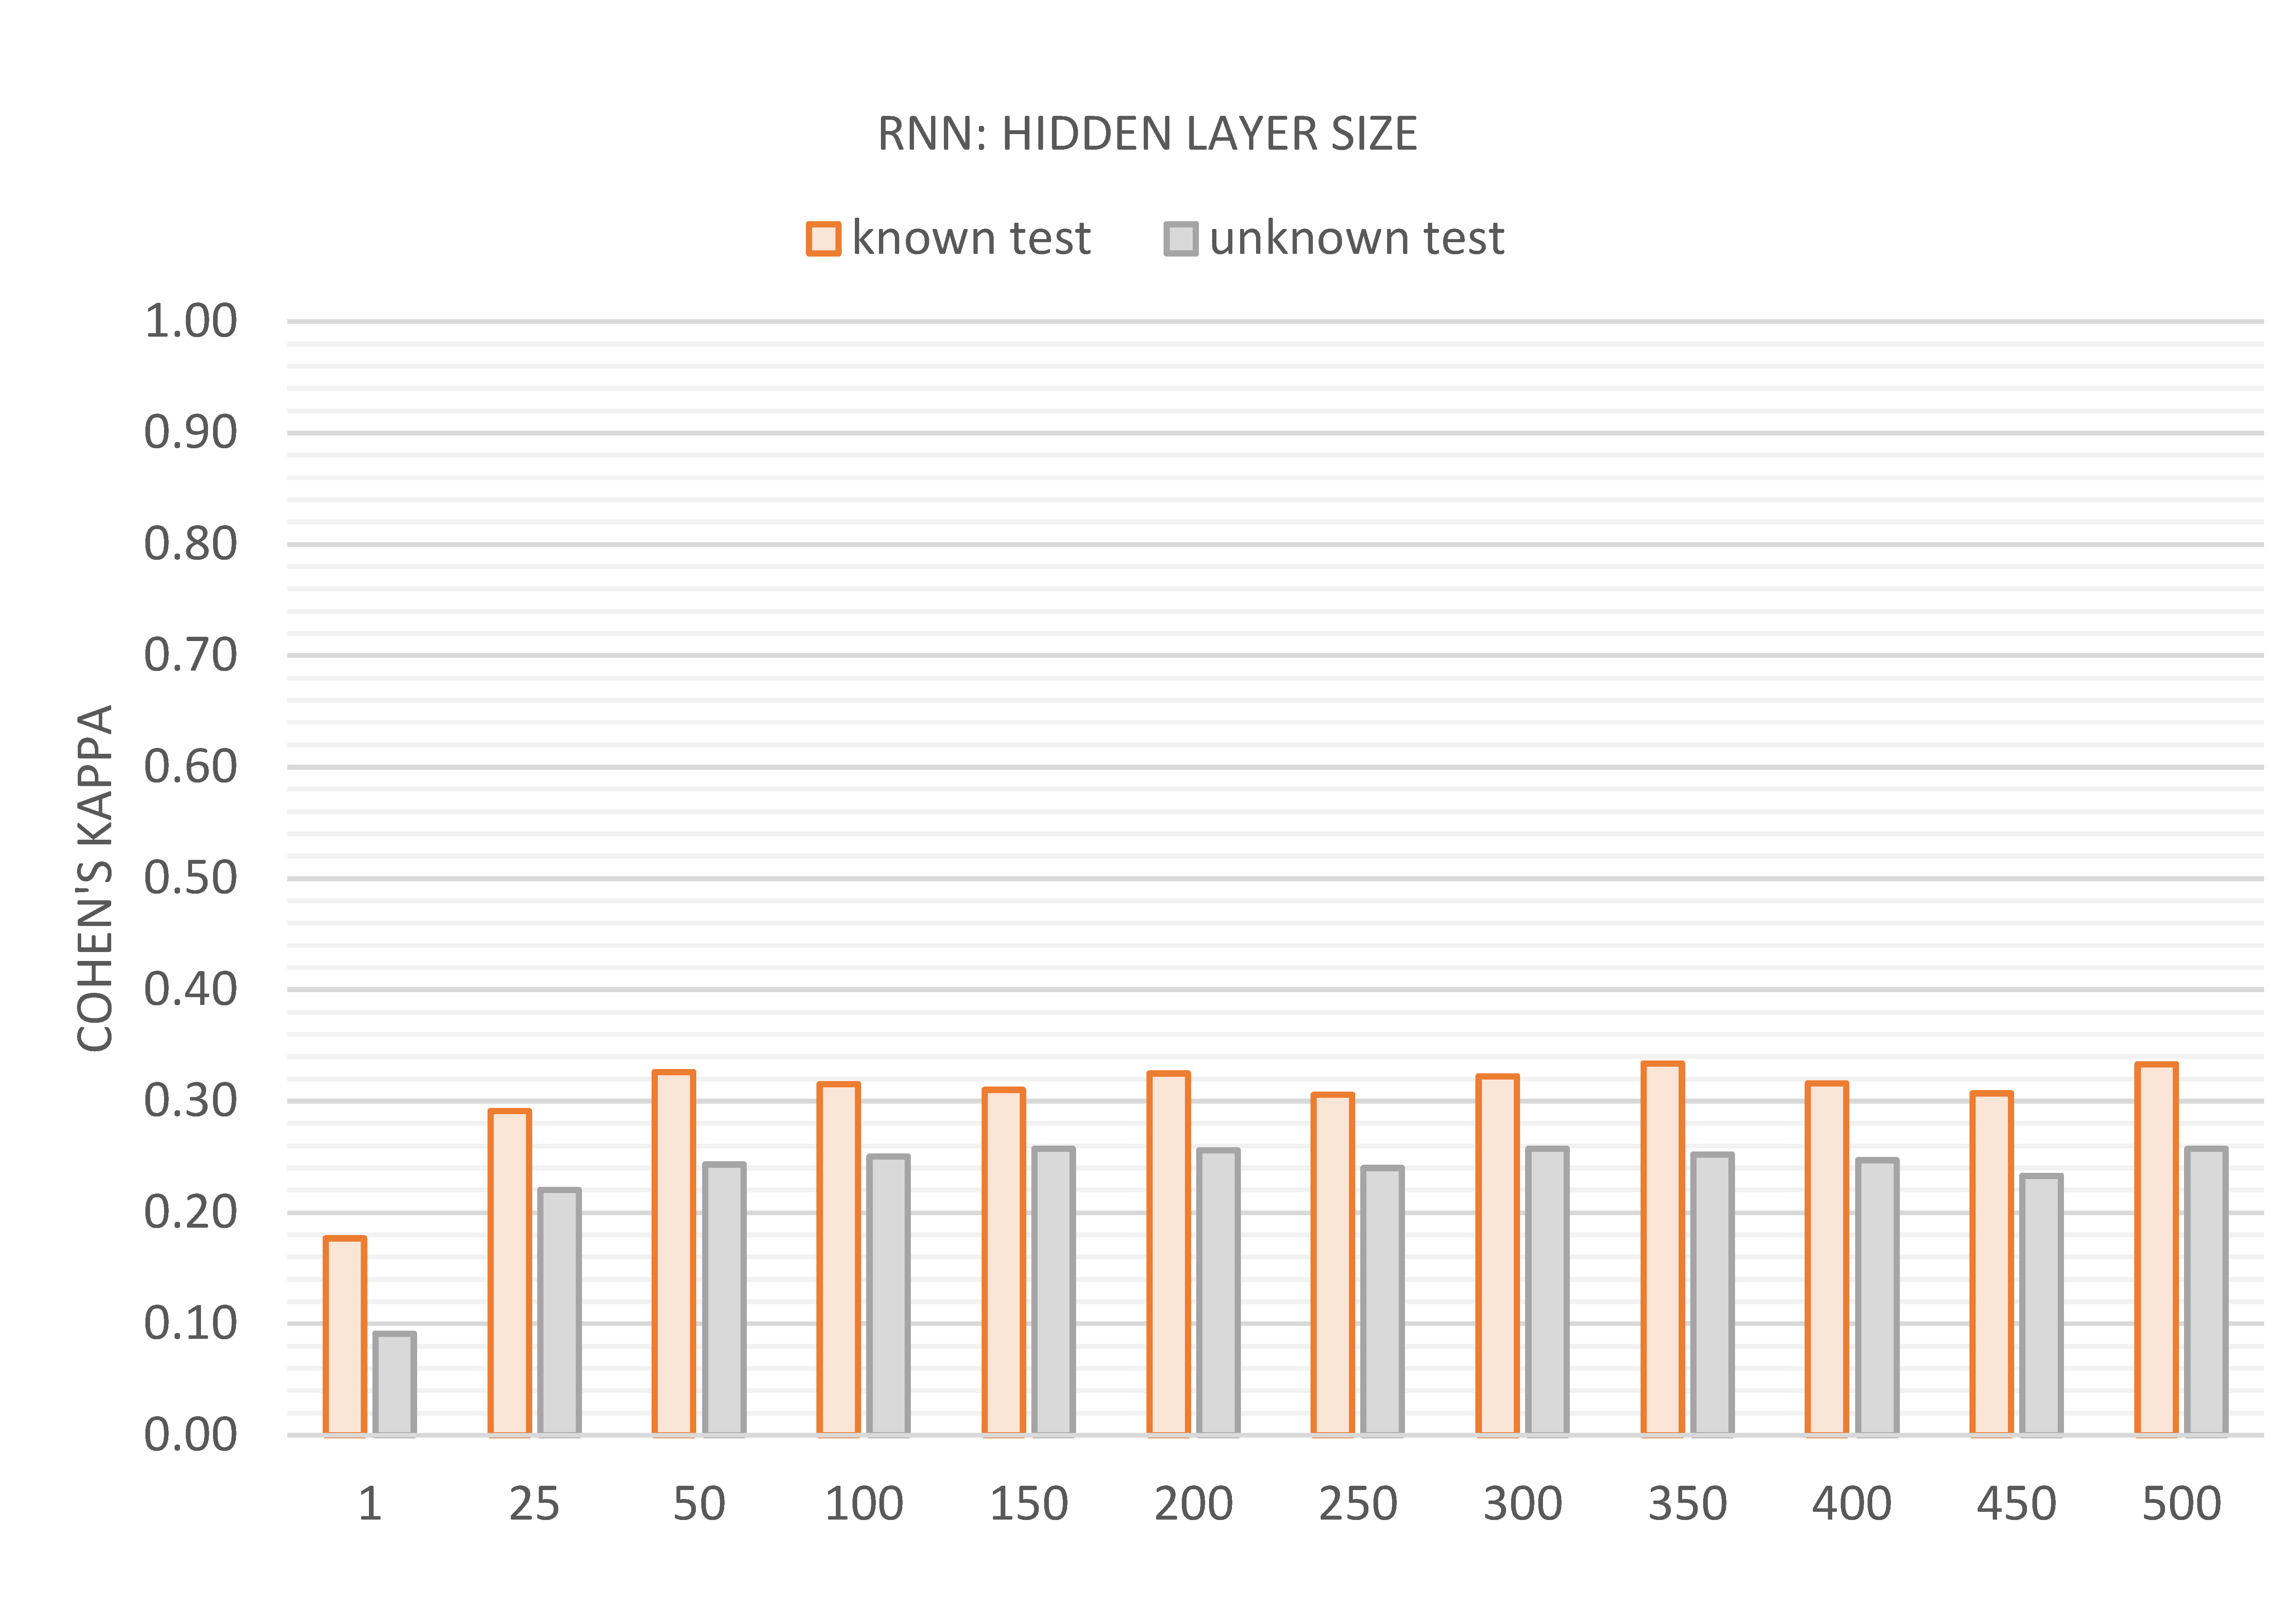
\includegraphics[width=\textwidth]{images/evaluation_rnn_s_k}
	\caption[RNN Evaluation: Hidden Layer Size]{The evaluation results of the RNN: Cohen's Kappa for parameter $s$: the size of the hidden layer.}
	\label{f.evaluation.rnn.s.k}
\end{figure}

\vspace{-11mm}
\begin{figure}[H]
	\centering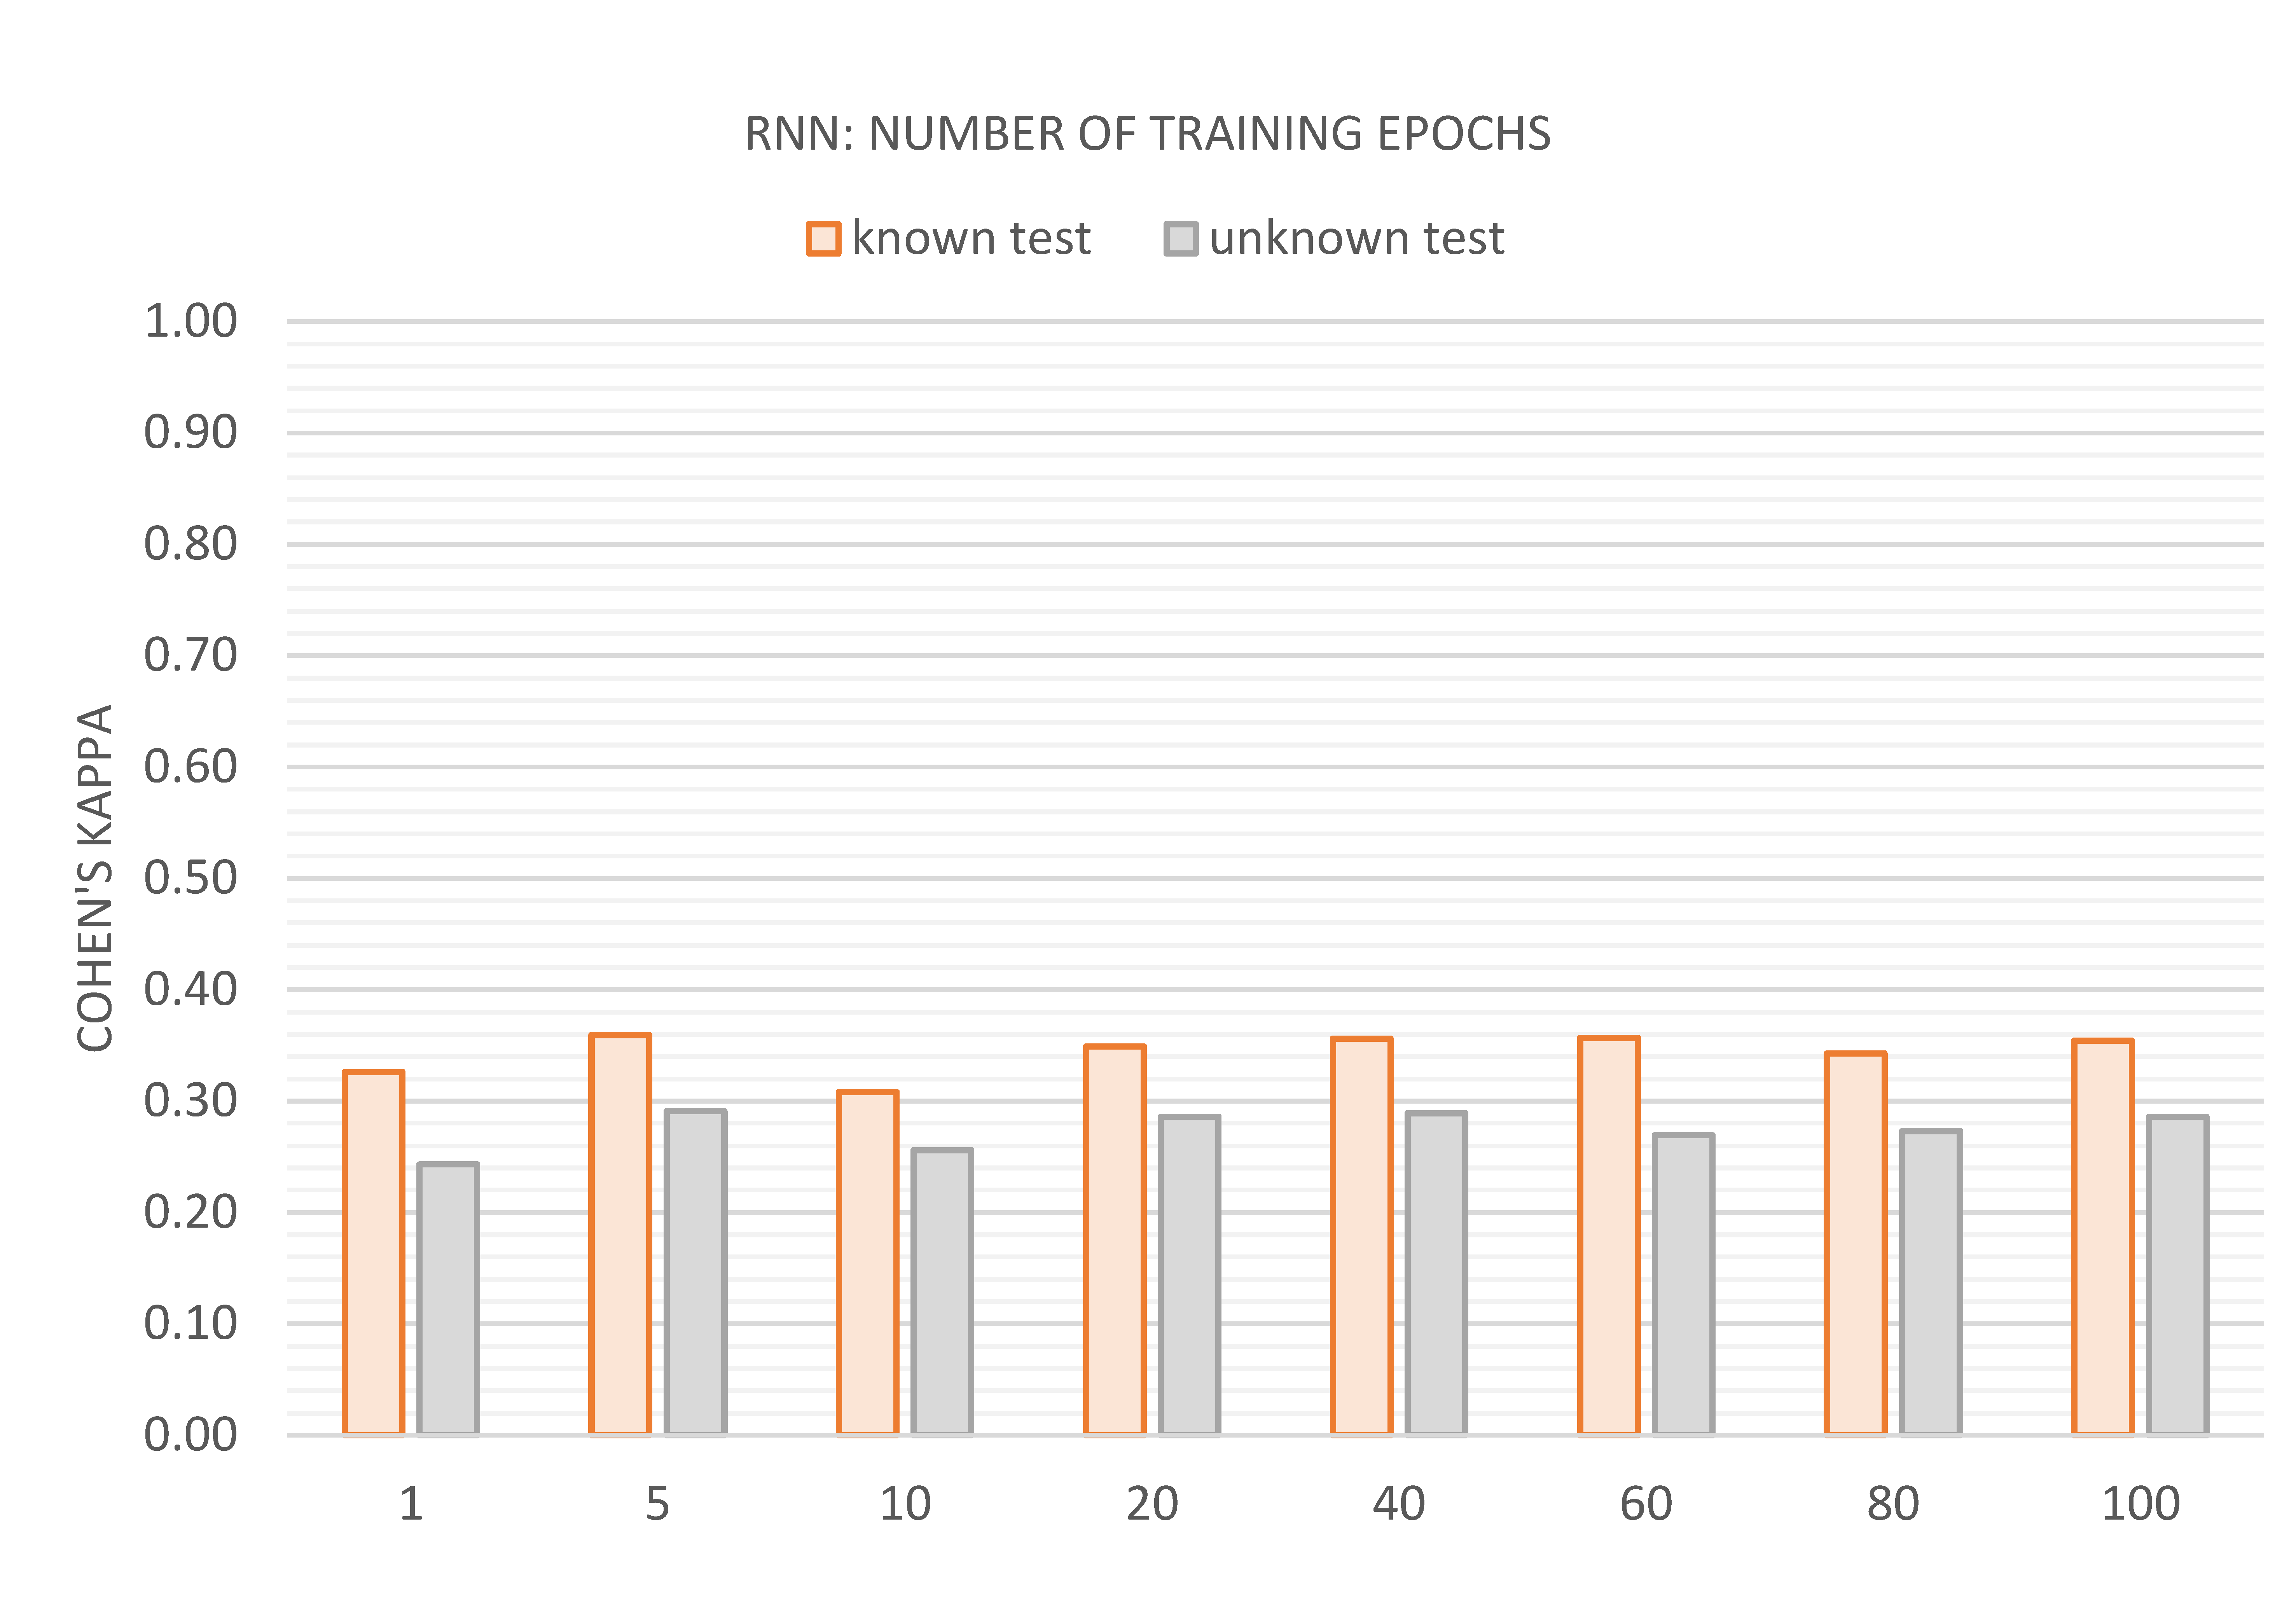
\includegraphics[width=\textwidth]{images/evaluation_rnn_n_k}
	\caption[RNN Evaluation: Number of Training Epochs]{The evaluation results of the RNN: Cohen's Kappa for parameter $n$: the number of training epochs.}
	\label{f.evaluation.rnn.n.k}
\end{figure}

\vspace{-11mm}
\begin{figure}[H]
	\centering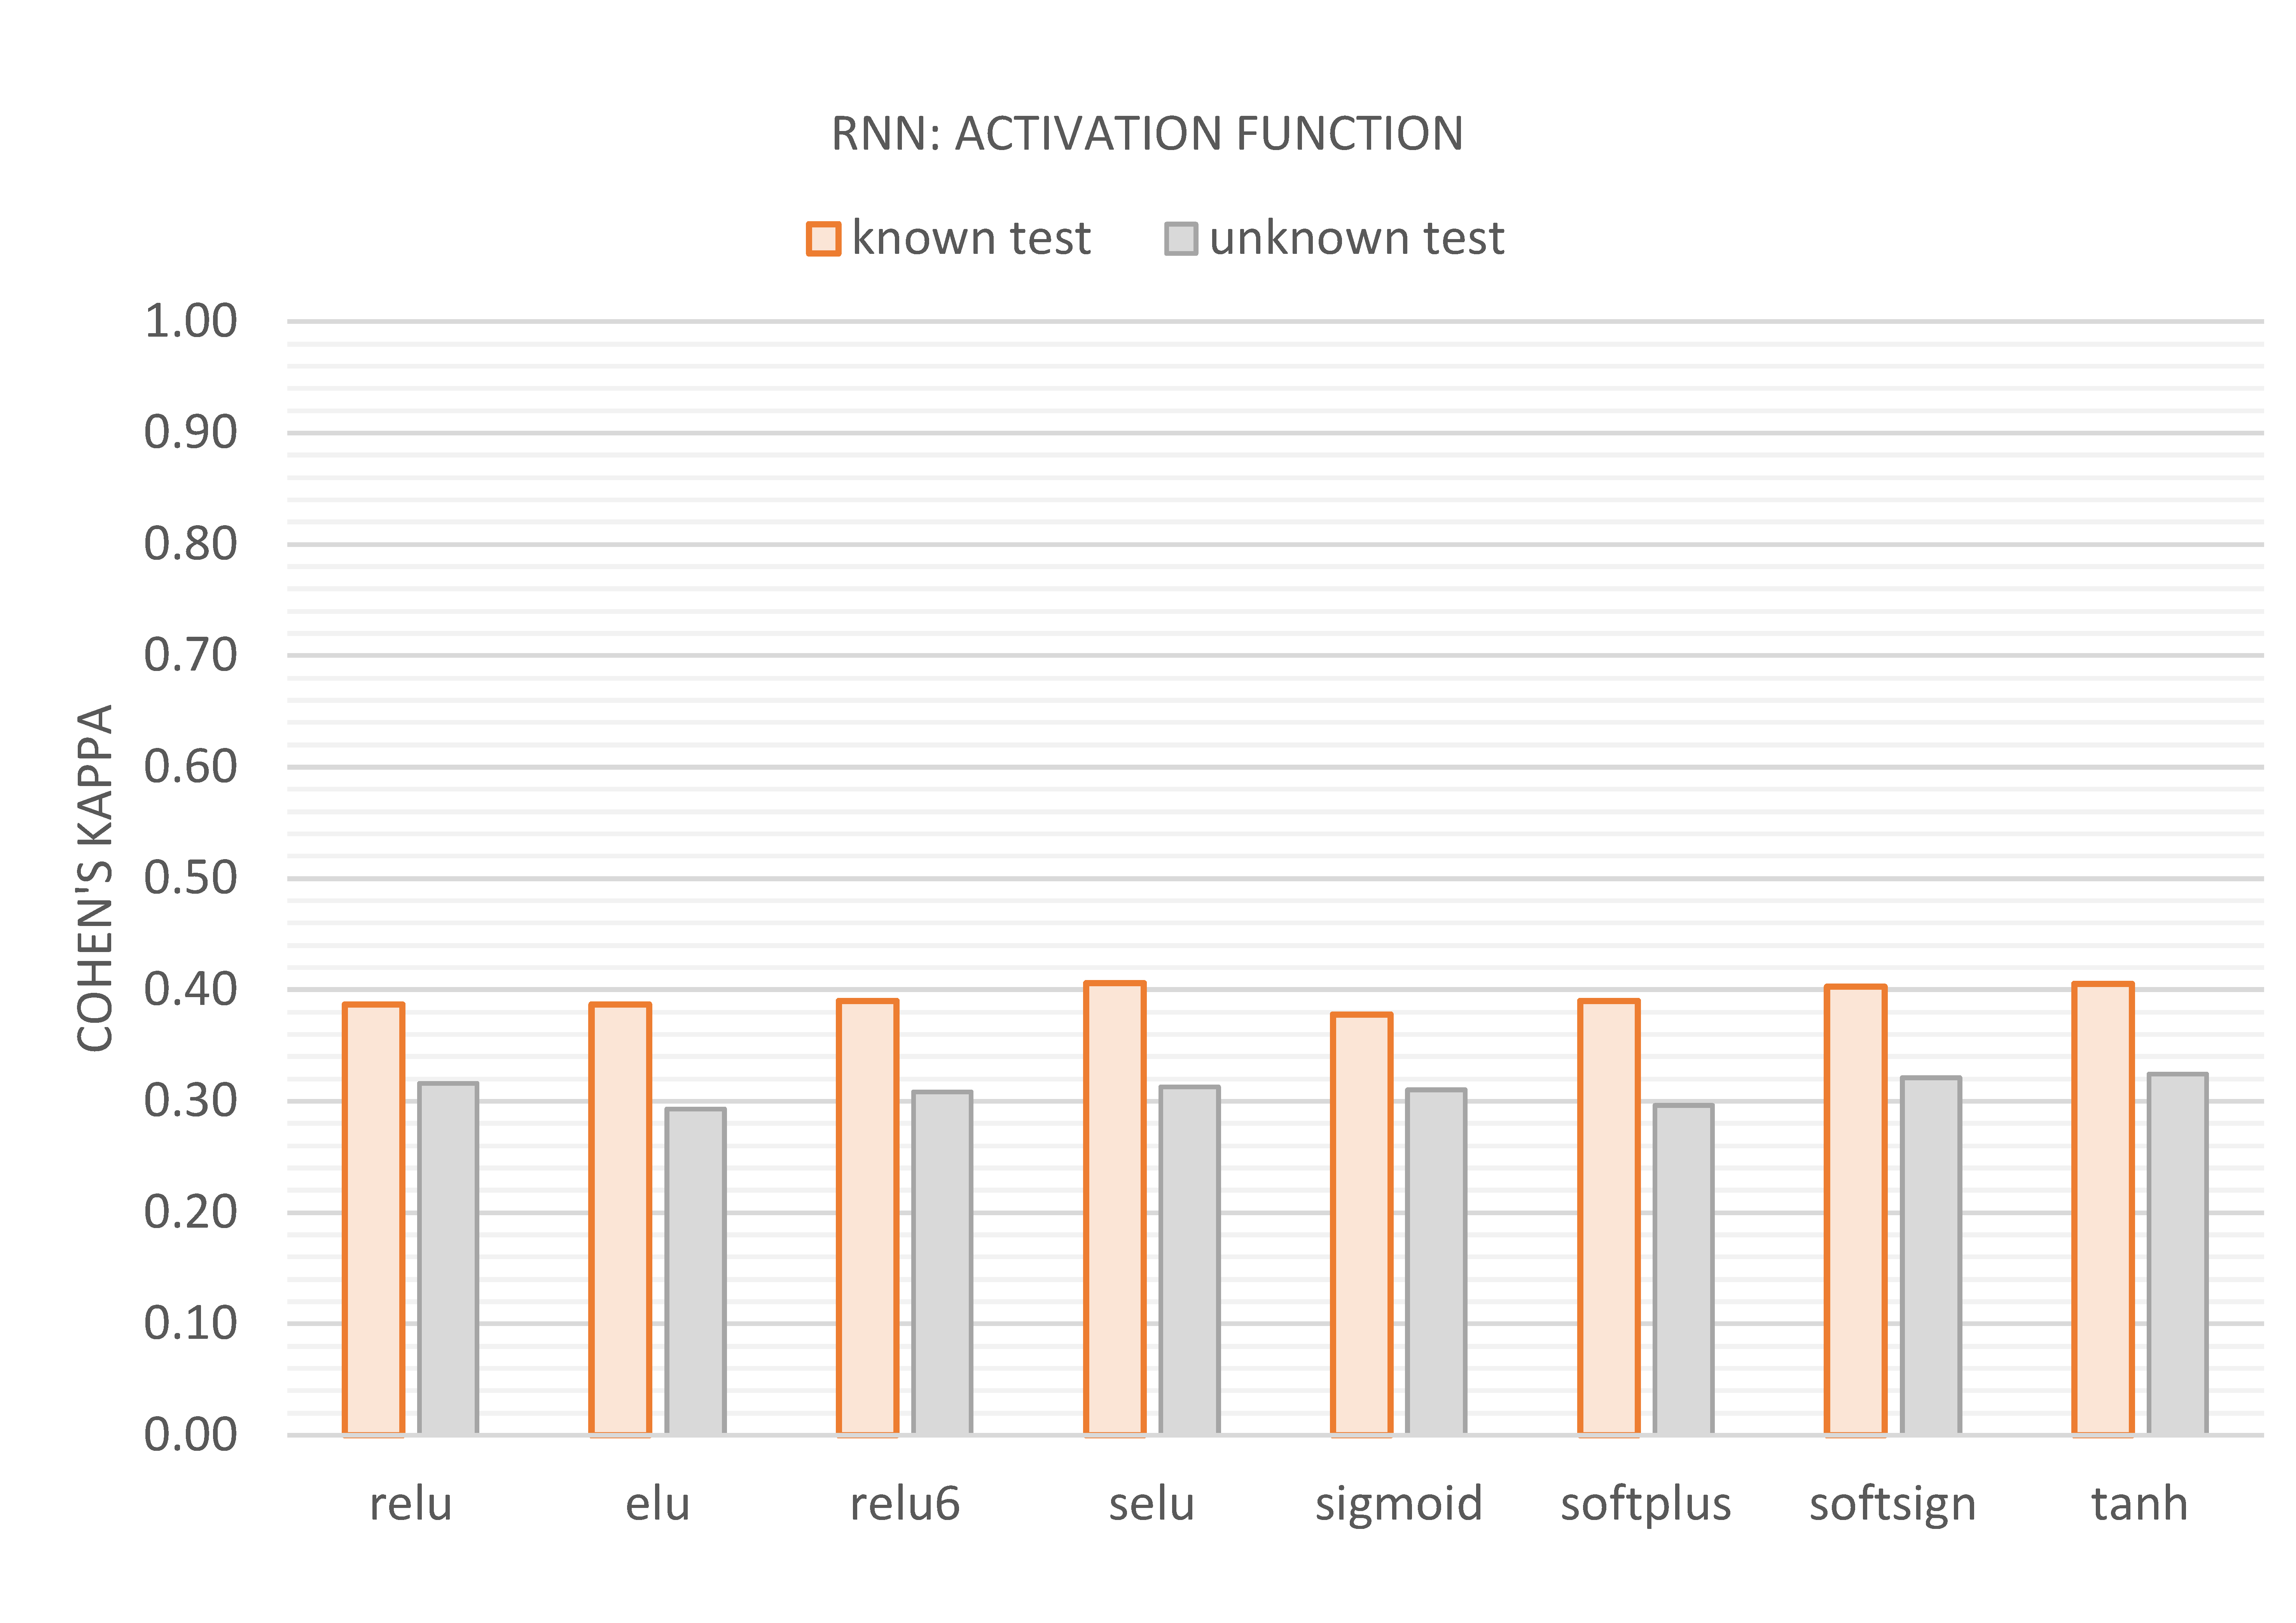
\includegraphics[width=\textwidth]{images/evaluation_rnn_a_k}
	\caption[RNN Evaluation: Activation Function]{The evaluation results of the RNN: Cohen's Kappa for parameter $a$: the type of the activation function.}
	\label{f.evaluation.rnn.a.k}
\end{figure}

\end{document}